%%% Hlavní soubor. Zde se definují základní parametry a odkazuje se na ostatní části. %%%

%% Verze pro jednostranný tisk:
% Okraje: levý 40mm, pravý 25mm, horní a dolní 25mm
% (ale pozor, LaTeX si sám přidává 1in)
\documentclass[12pt,a4paper]{report}
\setlength\textwidth{145mm}
\setlength\textheight{247mm}
\setlength\oddsidemargin{15mm}
\setlength\evensidemargin{15mm}
\setlength\topmargin{0mm}
\setlength\headsep{0mm}
\setlength\headheight{0mm}
\setlength{\emergencystretch}{5em}
 % \openright zařídí, aby následující text začínal na pravé straně knihy
\let\openright=\clearpage

%% Pokud tiskneme oboustranně:
% \documentclass[12pt,a4paper,twoside,openright]{report}
% \setlength\textwidth{145mm}
% \setlength\textheight{247mm}
% \setlength\oddsidemargin{14.2mm}
% \setlength\evensidemargin{0mm}
% \setlength\topmargin{0mm}
% \setlength\headsep{0mm}
% \setlength\headheight{0mm}
% \let\openright=\cleardoublepage
% 
%

% Přepneme na českou sazbu
\usepackage[czech]{babel}
\usepackage[IL2]{fontenc}


%% Použité kódování znaků: obvykle latin2, cp1250 nebo utf8:
\usepackage[utf8]{inputenc}

%%% Další užitečné balíčky (jsou součástí běžných distribucí LaTeXu)
\usepackage{amsmath}        % rozšíření pro sazbu matematiky
\usepackage{amsfonts}       % matematické fonty
\usepackage{amsthm}         % sazba vět, definic apod.
\usepackage{bbding}         % balíček s nejrůznějšími symboly
			    % (čtverečky, hvězdičky, tužtičky, nůžtičky, ...)
\usepackage{bm}             % tučné symboly (příkaz \bm)
\usepackage{graphicx}       % vkládání obrázků
\usepackage{caption}
\usepackage{subcaption}
\usepackage{fancyvrb}       % vylepšené prostředí pro strojové písmo
\usepackage{indentfirst}    % zavede odsazení 1. odstavce kapitoly
\usepackage[numbers]{natbib}         % zajištuje možnost odkazovat na literaturu

			    % stylem AUTOR (ROK), resp. AUTOR [ČÍSLO]
\usepackage[nottoc]{tocbibind} % zajistí přidání seznamu literatury,
                            % obrázků a tabulek do obsahu
\usepackage{icomma}         % inteligetní čárka v matematickém módu
\usepackage{dcolumn}        % lepší zarovnání sloupců v tabulkách
\usepackage{booktabs}       % lepší vodorovné linky v tabulkách
\usepackage{paralist}       % lepší enumerate a itemize
\usepackage[usenames]{xcolor}  % barevná sazba
\usepackage{textcomp}
\usepackage{float}
\usepackage{enumitem}
\usepackage{amssymb}

\raggedbottom


%%% Údaje o práci

% Název práce v jazyce práce (přesně podle zadání)
\def\NazevPrace{Hra Dungeon Master pro platformu .NET}

% Název práce v angličtině
\def\NazevPraceEN{Dungeon Master Game for the .NET Platform}

% Jméno autora
\def\AutorPrace{Petr Geiger}

% Rok odevzdání
\def\RokOdevzdani{2016}

% Název katedry nebo ústavu, kde byla práce oficiálně zadána
% (dle Organizační struktury MFF UK, případně plný název pracoviště mimo MFF)
\def\Katedra{Katedra distribuovaných a spolehlivých systémů}
\def\KatedraEN{Department of Distributed and Dependable Systems}

% Jedná se o katedru (department) nebo o ústav (institute)?
\def\TypPracoviste{Katedra}
\def\TypPracovisteEN{Department}

% Vedoucí práce: Jméno a příjmení s~tituly
\def\Vedouci{Mgr. Pavel Ježek, Ph.D.}

% Pracoviště vedoucího (opět dle Organizační struktury MFF)
\def\KatedraVedouciho{Katedra distribuovaných a spolehlivých systémů}
\def\KatedraVedoucihoEN{Department of Distributed and Dependable Systems}

% Studijní program a obor
\def\StudijniProgram{Informatika}
\def\StudijniObor{Programovaní a softwarové systémy}

% Nepovinné poděkování (vedoucímu práce, konzultantovi, tomu, kdo
% zapůjčil software, literaturu apod.)
\def\Podekovani{%
Děkuji svému vedoucímu práce Mgr. Pavlu Ježkovi, Ph. D. jak za pomoc s výběrem práce, tak za cenné rady při její tvorbě.
}

% Abstrakt (doporučený rozsah cca 80-200 slov; nejedná se o zadání práce)
\def\Abstrakt{%
Cílem bakalářské práce je reimplementovat hru Dungeon Master. V současné době existuje již několik klonů této 
známé hry. Nicméně oproti nim se tato práce zaměřuje především na následující aspekty. Hra je naprogramována 
v jazyce C\# s využitím platformy .NET. Dále celý engine je navrhnutý směrem k udržitelnosti a rozšiřitelnosti. 
Tzn. s využitím tohoto enginu je možné naprogramovat i jinou hru založenou na podobných základech. Ale 
především je jednoduché přidávat do enginu nové funkce. Engine je také 
připravený na rozdílné vstupní formáty herních úrovní. Dále je také kompletně oddělena zobrazovací vrstva. Vzhledem 
k povaze projektu by engine měl sloužit jako ukázkový příklad použitelný pro vzdělávání.

}
\def\AbstraktEN{%
The aim of this thesis is to reimplement the game Dungeon Master. There are currently several 
clones of this wellknown game. However, compared to them this work focuses on the following aspects.
The game is programmed in C\# using .NET platform. Furthermore, the entire engine is designed
towards sustainability and scalability. That means that by using this engine it is possible to program 
slightly differrent game based on the same basics. Especially, it is easy to add new features to the
engine. The engine is also prepared for different input formats of levels. Also the rendering layer
of the game engine is completely separate. Due to nature of the project the engine should serve as prime example
used for education.
}

% 3 až 5 klíčových slov (doporučeno), každé uzavřeno ve složených závorkách
\def\KlicovaSlova{%
{RPG} {Dungeon Master} {Architektura softwaru} {vzdělávání}
}
\def\KlicovaSlovaEN{%
{RPG} {Dungeon Master} {Software architecture} {education}
}

%% Balíček hyperref, kterým jdou vyrábět klikací odkazy v PDF,
%% ale hlavně ho používáme k uložení metadat do PDF (včetně obsahu).
\usepackage[pdftex,unicode]{hyperref}   % Musí být za všemi ostatními balíčky
\hypersetup{breaklinks=true}
\hypersetup{pdftitle={\NazevPrace}}
\hypersetup{pdfauthor={\AutorPrace}}
\hypersetup{pdfkeywords=\KlicovaSlova}
\hypersetup{urlcolor=blue}

\newcommand{\ccc}[1]{{\mbox{\fontfamily{lmtt}\selectfont\textbf{#1}}}}
\newcommand{\xxx}[1]{\textit{#1}}
\newcommand{\cc}[1]{(viz obr. \ref{#1})}
\newcommand{\vref}[1]{(viz sekce \ref{#1})}
\newcommand{\vbref}[1]{(viz bod \ref{#1})}
\newcommand{\aref}[1]{(viz cíl práce \ref{#1})}

\renewcommand{\labelitemii}{$\circ$}
\renewcommand\labelitemiii{$\diamond$}

\newcommand{\imgx}[2]{\begin{figure}[H]\centering
\includegraphics[width=\textwidth]{./img/#1}
\caption{#2}
\label{#1}
\end{figure}}


%% Definice různých užitečných maker (viz popis uvnitř souboru)
%%% Tento soubor obsahuje definice různých užitečných maker a prostředí %%%
%%% Další makra připisujte sem, ať nepřekáží v ostatních souborech.     %%%

%%% Drobné úpravy stylu

% Tato makra přesvědčují mírně ošklivým trikem LaTeX, aby hlavičky kapitol
% sázel příčetněji a nevynechával nad nimi spoustu místa. Směle ignorujte.
\makeatletter
\def\@makechapterhead#1{
  {\parindent \z@ \raggedright \normalfont
   \Huge\bfseries \thechapter. #1
   \par\nobreak
   \vskip 20\p@
}}
\def\@makeschapterhead#1{
  {\parindent \z@ \raggedright \normalfont
   \Huge\bfseries #1
   \par\nobreak
   \vskip 20\p@
}}
\makeatother

% Toto makro definuje kapitolu, která není očíslovaná, ale je uvedena v obsahu.
\def\chapwithtoc#1{
\chapter*{#1}
\addcontentsline{toc}{chapter}{#1}
}

% Trochu volnější nastavení dělení slov, než je default.
\lefthyphenmin=2
\righthyphenmin=2

% Zapne černé "slimáky" na koncích řádků, které přetekly, abychom si
% jich lépe všimli.
\overfullrule=1mm

%%% Makra pro definice, věty, tvrzení, příklady, ... (vyžaduje baliček amsthm)

\theoremstyle{plain}
\newtheorem{veta}{Věta}
\newtheorem{lemma}[veta]{Lemma}
\newtheorem{tvrz}[veta]{Tvrzení}

\theoremstyle{plain}
\newtheorem{definice}{Definice}

\theoremstyle{remark}
\newtheorem*{dusl}{Důsledek}
\newtheorem*{pozn}{Poznámka}
\newtheorem*{prikl}{Příklad}

%%% Prostředí pro důkazy

\newenvironment{dukaz}{
  \par\medskip\noindent
  \textit{Důkaz}.
}{
\newline
\rightline{$\square$}  % nebo \SquareCastShadowBottomRight z balíčku bbding
}

%%% Prostředí pro sazbu kódu, případně vstupu/výstupu počítačových
%%% programů. (Vyžaduje balíček fancyvrb -- fancy verbatim.)

\DefineVerbatimEnvironment{code}{Verbatim}{fontsize=\small, frame=single}

%%% Prostor reálných, resp. přirozených čísel
\newcommand{\R}{\mathbb{R}}
\newcommand{\N}{\mathbb{N}}

%%% Užitečné operátory pro statistiku a pravděpodobnost
\DeclareMathOperator{\pr}{\textsf{P}}
\DeclareMathOperator{\E}{\textsf{E}\,}
\DeclareMathOperator{\var}{\textrm{var}}
\DeclareMathOperator{\sd}{\textrm{sd}}

%%% Příkaz pro transpozici vektoru/matice
\newcommand{\T}[1]{#1^\top}

%%% Vychytávky pro matematiku
\newcommand{\goto}{\rightarrow}
\newcommand{\gotop}{\stackrel{P}{\longrightarrow}}
\newcommand{\maon}[1]{o(n^{#1})}
\newcommand{\abs}[1]{\left|{#1}\right|}
\newcommand{\dint}{\int_0^\tau\!\!\int_0^\tau}
\newcommand{\isqr}[1]{\frac{1}{\sqrt{#1}}}

%%% Vychytávky pro tabulky
\newcommand{\pulrad}[1]{\raisebox{1.5ex}[0pt]{#1}}
\newcommand{\mc}[1]{\multicolumn{1}{c}{#1}}


%% Titulní strana a různé povinné informační strany

\begin{document}

%%% Titulní strana práce a další povinné informační strany

%%% Titulní strana práce

\pagestyle{empty}
\hypersetup{pageanchor=false}

\begin{center}

\large

Univerzita Karlova v Praze

\medskip

Matematicko-fyzikální fakulta

\vfill

{\bf\Large BAKALÁŘSKÁ PRÁCE}

\vfill

\centerline{\mbox{\includegraphics[width=60mm]{./img/logo.pdf}}}

\vfill
\vspace{5mm}

{\LARGE\AutorPrace}

\vspace{15mm}

{\LARGE\bfseries\NazevPrace}

\vfill

\Katedra

\vfill

\begin{tabular}{rl}

Vedoucí bakalářské práce: & \Vedouci \\
\noalign{\vspace{2mm}}
Studijní program: & \StudijniProgram \\
\noalign{\vspace{2mm}}
Studijní obor: & \StudijniObor \\
\end{tabular}

\vfill

% Zde doplňte rok
Praha \RokOdevzdani

\end{center}

\newpage

%%% Následuje vevázaný list -- kopie podepsaného "Zadání bakalářské práce".
%%% Toto zadání NENÍ součástí elektronické verze práce, nescanovat.

%%% Strana s čestným prohlášením k bakalářské práci

\openright
\hypersetup{pageanchor=true}
\pagestyle{plain}
\pagenumbering{roman}
\vglue 0pt plus 1fill

\noindent
Prohlašuji, že jsem tuto bakalářskou práci vypracoval(a) samostatně a výhradně
s~použitím citovaných pramenů, literatury a dalších odborných zdrojů.

\medskip\noindent
Beru na~vědomí, že se na moji práci vztahují práva a povinnosti vyplývající
ze zákona č. 121/2000 Sb., autorského zákona v~platném znění, zejména skutečnost,
že Univerzita Karlova v Praze má právo na~uzavření licenční smlouvy o~užití této
práce jako školního díla podle §60 odst. 1 autorského zákona.

\vspace{10mm}

\hbox{\hbox to 0.5\hsize{%
V ........ dne ............
\hss}\hbox to 0.5\hsize{%
Podpis autora
\hss}}

\vspace{20mm}
\newpage

%%% Povinná informační strana bakalářské práce

\openright

\vbox to 0.5\vsize{
\setlength\parindent{0mm}
\setlength\parskip{5mm}

Název práce:
\NazevPrace

Autor:
\AutorPrace

\TypPracoviste:
\Katedra

Vedoucí bakalářské práce:
\Vedouci, \KatedraVedouciho

Abstrakt:
\Abstrakt

Klíčová slova:
\KlicovaSlova

\vss}\nobreak\vbox to 0.49\vsize{
\setlength\parindent{0mm}
\setlength\parskip{5mm}

Title:
\NazevPraceEN

Author:
\AutorPrace

\TypPracovisteEN:
\KatedraEN

Supervisor:
\Vedouci, \KatedraVedoucihoEN

Abstract:
\AbstraktEN

Keywords:
\KlicovaSlovaEN

\vss}

\newpage

%%% Poděkování

\openright

\noindent
\Podekovani

\newpage

\openright
\pagestyle{plain}
\pagenumbering{arabic}
\setcounter{page}{1}


%%% Strana s automaticky generovaným obsahem bakalářské práce

\tableofcontents

%%% Jednotlivé kapitoly práce jsou pro přehlednost uloženy v samostatných souborech
%%%\chapter*{Úvod}
\addcontentsline{toc}{chapter}{Úvod}

Následuje několik ukázkových kapitol, které doporučují, jak by se
měla bakalářská práce sázet. Primárně popisují použití \TeX{}ové
šablony, ale obecné rady poslouží dobře i~uživatelům jiných
systémů.

%%%%%% Fiktivní kapitola s ukázkami sazby

\chapter{Nápověda k~sazbě}

\section{Úprava práce}

Vlastní text bakalářské práce je uspořádaný hierarchicky do kapitol a podkapitol,
každá kapitola začíná na nové straně. Text je zarovnán do bloku. Nový odstavec
se obvykle odděluje malou vertikální mezerou a odsazením prvního řádku. Grafická
úprava má být v~celém textu jednotná.

Práce se tiskne na bílý papír formátu A4. Okraje musí ponechat dost místa na vazbu:
doporučen je horní, dolní a pravý okraj $25\,\rm mm$, levý okraj $40\,\rm mm$.
Číslují se všechny strany kromě obálky a informačních stran na začátku práce;
první číslovaná strana bývá obvykle ta s~obsahem.

Písmo se doporučuje dvanáctibodové ($12\,\rm pt$) se standardní vzdáleností mezi řádky
(pokud píšete ve Wordu nebo podobném programu, odpovídá tomu řádkování $1,5$; v~\TeX{}u
není potřeba nic přepínat). Pro běžný text používejte vzpřímené patkové písmo.
Text matematických vět se obvykle tiskne pro zdůraznění skloněným (slanted) písmem,
není-li k~dispozici, může být zastoupeno kurzívou.

Primárně je doporučován jednostranný tisk (příliš tenkou práci lze obtížně svázat).
Delší práce je lepší tisknout oboustranně a přizpůsobit tomu velikosti okrajů:
$40\,\rm mm$ má vždy \emph{vnitřní} okraj. Rub titulního listu zůstává nepotištěný.

Zkratky použité v textu musí být vysvětleny vždy u prvního výskytu zkratky (v~závorce nebo
v poznámce pod čarou, jde-li o složitější vysvětlení pojmu či zkratky). Pokud je zkratek
více, připojuje se seznam použitých zkratek, včetně jejich vysvětlení a/nebo odkazů
na definici.

Delší převzatý text jiného autora je nutné vymezit uvozovkami nebo jinak vyznačit a řádně
citovat.

\section{Jednoduché příklady}

Čísla v~českém textu obvykle sázíme v~matematickém režimu s~desetinnou čárkou:
%%% Bez \usepackage{icomma}:
% $\pi \doteq 3{,}141\,592\,653\,589$.
%%% S \usepackage{icomma}:
$\pi \doteq 3,141\,592\,653\,589$.
V~matematických textech se považuje za přípustné používat desetinnou tečku
(pro lepší odlišení od čárky v~roli oddělovače). Numerické výsledky se uvádějí
s~přiměřeným počtem desetinných míst.

Mezi číslo a jednotku patří úzká mezera: šířka stránky A4 činí $210\,\rm mm$, což si
pamatuje pouze $5\,\%$ autorů. Pokud ale údaj slouží jako přívlastek, mezeru vynecháváme:
$25\rm mm$ okraj, $95\%$ interval spolehlivosti.

Rozlišujeme různé druhy pomlček:
červeno-černý (krátká pomlčka),
strana 16--22 (střední),
$45-44$ (matematické minus),
a~toto je --- jak se asi dalo čekat --- vložená věta ohraničená dlouhými pomlčkami.

V~českém textu se používají \uv{české} uvozovky, nikoliv ``anglické''.

% V tomto odstavci se vlnka zviditelňuje
{
\def~{{\tt\char126}}
Na některých místech je potřeba zabránit lámání řádku (v~\TeX{}u značíme vlnovkou):
u~předložek (neslabičnych, nebo obecně jednopísmenných), vrchol~$v$, před $k$~kroky,
a~proto, \dots{} obecně kdekoliv, kde by při rozlomení čtenář \uv{škobrtnul}.
}

\section{Matematické vzorce a výrazy}

Proměnné sázíme kurzívou (to \TeX{} v~matematickém módu dělá sám, ale
nezapomínejte na to v~okolním textu a také si matematický mód zapněte).
Názvy funkcí sázíme vzpřímeně. Tedy například:
$\var(X) = \E X^2 - \bigl(\E X \bigr)^2$.

Zlomky uvnitř odstavce (třeba $\frac{5}{7}$ nebo $\frac{x+y}{2}$) mohou
být příliš stísněné, takže je lepší sázet jednoduché zlomky s~lomítkem:
$5/7$, $(x+y)/2$.

Nechť
\[   % LaTeXová náhrada klasického TeXového $$
\mathbb{X} = \begin{pmatrix}
      \T{\bm x_1} \\
      \vdots \\
      \T{\bm x_n}
      \end{pmatrix}.
\]
Povšimněme si tečky za~maticí. Byť je matematický text vysázen
ve~specifickém prostředí, stále je gramaticky součástí věty a~tudíž je
zapotřebí neopomenout patřičná interpunkční znaménka. Výrazy, na které
chceme později odkazovat, je vhodné očíslovat:
\begin{equation}\label{eq01:Xmat}
\mathbb{X} = \begin{pmatrix}
      \T{\bm x_1} \\
      \vdots \\
      \T{\bm x_n}
      \end{pmatrix}.
\end{equation}
Výraz \eqref{eq01:Xmat} definuje matici $\mathbb{X}$. Pro lepší čitelnost
a~přehlednost textu je vhodné číslovat pouze ty výrazy, na které se
autor někde v~další části textu odkazuje. To jest, nečíslujte
automaticky všechny výrazy vysázené některým z~matematických
prostředí.

Zarovnání vzorců do několika sloupečků:
\begin{alignat*}{3}
S(t) &= \pr(T > t),    &\qquad t&>0       &\qquad&\text{ (zprava spojitá),}\\
F(t) &= \pr(T \leq t), &\qquad t&>0       &\qquad&\text{ (zprava spojitá).}
\end{alignat*}

Dva vzorce se spojovníkem:
\begin{equation}\label{eq01:FS}
\left.
\begin{aligned}
S(t) &= \pr(T > t) \\[1ex]
F(t) &= \pr(T \leq t)
\end{aligned}
\;	% zde pomůže ručně vynechat trochu místa
\right\}
\quad t>0 \qquad \text{(zprava spojité).}
\end{equation}

Dva centrované nečíslované vzorce:
\begin{gather*}
\bm Y = \mathbb{X}\bm\beta + \bm\varepsilon, \\[1ex]
\mathbb{X} = \begin{pmatrix} 1 & \T{\bm x_1} \\ \vdots & \vdots \\ 1 &
  \T{\bm x_n} \end{pmatrix}.
\end{gather*}
Dva centrované číslované vzorce:
\begin{gather}
\bm Y = \mathbb{X}\bm\beta + \bm\varepsilon, \label{eq02:Y}\\[1ex]
\mathbb{X} = \begin{pmatrix} 1 & \T{\bm x_1} \label{eq03:X}\\ \vdots & \vdots \\ 1 &
  \T{\bm x_n} \end{pmatrix}.
\end{gather}

Definice rozdělená na dva případy:
\[
P_{r-j}=
\begin{cases}
0, & \text{je-li $r-j$ liché},\\
r!\,(-1)^{(r-j)/2}, & \text{je-li $r-j$ sudé}.
\end{cases}
\]
Všimněte si použití interpunkce v této konstrukci. Čárky a tečky se
dávají na místa, kam podle jazykových pravidel patří.

\begin{align}
x& = y_1-y_2+y_3-y_5+y_8-\dots = && \text{z \eqref{eq02:Y}} \nonumber\\
& = y'\circ y^* = && \text{podle \eqref{eq03:X}} \nonumber\\
& = y(0) y' && \text {z Axiomu 1.}
\end{align}


Dva zarovnané vzorce nečíslované:
\begin{align*}
L(\bm\theta) &= \prod_{i=1}^n f_i(y_i;\,\bm\theta), \\
\ell(\bm\theta) &= \log\bigl\{L(\bm\theta)\bigr\} =
\sum_{i=1}^n \log\bigl\{f_i(y_i;\,\bm\theta)\bigr\}.
\end{align*}
Dva zarovnané vzorce, první číslovaný:
\begin{align}
L(\bm\theta) &= \prod_{i=1}^n f_i(y_i;\,\bm\theta), \label{eq01:L} \\
\ell(\bm\theta) &= \log\bigl\{L(\bm\theta)\bigr\} =
\sum_{i=1}^n \log\bigl\{f_i(y_i;\,\bm\theta)\bigr\}. \nonumber
\end{align}

Vzorec na dva řádky, první řádek zarovnaný vlevo, druhý vpravo, nečíslovaný:
\begin{multline*}
\ell(\mu,\,\sigma^2) = \log\bigl\{L(\mu,\,\sigma^2)\bigr\} =
\sum_{i=1}^n \log\bigl\{f_i(y_i;\,\mu,\,\sigma^2)\bigr\}= \\
  = -\,\frac{n}{2}\,\log(2\pi\sigma^2) \,-\,
\frac{1}{2\sigma^2}\sum_{i=1}^n\,(y_i - \mu)^2.
\end{multline*}

Vzorec na dva řádky, zarovnaný na $=$, číslovaný uprostřed:
\begin{equation}\label{eq01:ell}
\begin{split}
\ell(\mu,\,\sigma^2) &= \log\bigl\{L(\mu,\,\sigma^2)\bigr\} =
\sum_{i=1}^n \log\bigl\{f(y_i;\,\mu,\,\sigma^2)\bigr\}= \\
& = -\,\frac{n}{2}\,\log(2\pi\sigma^2) \,-\,
\frac{1}{2\sigma^2}\sum_{i=1}^n\,(y_i - \mu)^2.
\end{split}
\end{equation}

\section{Definice, věty, důkazy, \dots}

Konstrukce typu definice, věta, důkaz, příklad, \dots je vhodné
odlišit od okolního textu a~případně též číslovat s~možností použití
křížových odkazů. Pro každý typ těchto konstrukcí je vhodné mít
v~souboru s~makry (\texttt{makra.tex}) nadefinované jedno prostředí,
které zajistí jak vizuální odlišení od okolního textu, tak
automatické číslování s~možností křížově odkazovat.

\begin{definice}\label{def01:1}
  Nechť náhodné veličiny $X_1,\dots,X_n$ jsou definovány na témž
  prav\-dě\-po\-dob\-nost\-ním prostoru $(\Omega,\,\mathcal{A},\,\pr)$. Pak
  vektor $\bm X = \T{(X_1,\dots,X_n)}$ nazveme \emph{náhodným
    vektorem}.
\end{definice}

\begin{definice}[náhodný vektor]\label{def01:2}
  Nechť náhodné veličiny $X_1,\dots,X_n$ jsou definovány na témž
  pravděpodobnostním prostoru $(\Omega,\,\mathcal{A},\,\pr)$. Pak
  vektor $\bm X = \T{(X_1,\dots,X_n)}$ nazveme \emph{náhodným
    vektorem}.
\end{definice}
Definice~\ref{def01:1} ukazuje použití prostředí pro sazbu definice
bez titulku, definice~\ref{def01:2} ukazuje použití prostředí pro
sazbu definice s~titulkem.

\begin{veta}\label{veta01:1}
  Náhodný vektor $\bm X$ je měřitelné zobrazení prostoru
  $(\Omega,\,\mathcal{A},\,\pr)$ do $(\R_n,\,\mathcal{B}_n)$.
\end{veta}

\begin{lemma}[\citealp{Andel07}, str. 29]\label{veta01:2}
  Náhodný vektor $\bm X$ je měřitelné zobrazení prostoru
  $(\Omega,\,\mathcal{A},\,\pr)$ do $(\R_n,\,\mathcal{B}_n)$.
\end{lemma}
\begin{dukaz}
  Jednotlivé kroky důkazu jsou podrobně popsány v~práci \citet[str.
  29]{Andel07}.
\end{dukaz}
Věta~\ref{veta01:1} ukazuje použití prostředí pro sazbu matematické
věty bez titulku, lemma~\ref{veta01:2} ukazuje použití prostředí pro
sazbu matematické věty s~titulkem. Lemmata byla zavedena v~hlavním
souboru tak, že sdílejí číslování s~větami.

\sloppy
\chapter{Úvod}

Dungeon Master je počítačová hra žánru RPG (role playing game) vyvinuta firmou Faster Then Light v roce 1987.
Byla to první real-time hra tohoto typu s pseudo 3D pohledem a ovládáním pomocí myši. Hráč má k dispozici skupinu až čtyř hrdinů,
s kterými prochází podzemní bludiště a bojuje s nepřáteli \cc{obr0:uvod}. Tito hrdinové se ve hře nazývají šampioni a mohou se 
zdokonalovat v různých dovednostech. 

\begin{figure}[H]\centering
\includegraphics[width=\textwidth]{./img/DM-original-screen.png}
\caption{Screenshot originální hry Dungeon Master}
\label{obr0:uvod}
\end{figure}

Bludiště se skládá z několika úrovní uspořádaných vertikálně pod sebou. 
Jednotlivé úrovně pak nemusí být stejně velké a mohou být od sebe různě horizontálně odsazené.
Každá úroveň je tvořena obdélníkovou plochou s pravidelnou mřížkou \cc{DM-levels}. Pole vymezena mřížkou nazýváme dlaždice a je jich 
ve hře několik typů, které definují jejích vzhled a funkci. Některé dlaždice lze aktivovat tzv. přepínači. Takové typy dlaždic
jsou například dveře nebo jáma \cc{obr0:uvod}, které lze takto otvírat či zavírat. Přepínače mohou být buď nášlapné na podlaze nebo aktivovatelné
pomocí myši na zdech. Mezi úrovněmi lze sestupovat pomocí dlaždic typu schody.  Dále je možné se teleportovat mezi dlaždicemi, a to i v různých úrovních, pomocí dlaždice
typu teleport. 

\imgx{DM-levels}{Ilustrace uspořádání herních úrovní.}

Hráč je na začátku postaven do nejvýše položené úrovně, kde si vybere svoji skupinu šampionů. 
Pohyb skupiny mezi dlaždicemi je zcela diskrétní, to znamená, že se nelze se skupinou zastavit mezi dlaždicemi, ale pohyb je vždy dokončen
až na vedlejší dlaždici. Se skupinou je tedy vždy asociována pouze jedna dlaždice. Na dlaždicích pak mohou
být různé předměty, které je možné sbírat. Šampioni mohou s předměty provádět různé akce.
Například se zbraněmi lze bojovat nebo lektvary je možné pít a zlepšit si tak dočasně vlastnosti. Kromě těchto 
akcí může ještě šampion vyvolávat kouzla. Nicméně k tomu potřebuje dostatečnou úroveň odpovídající dovednosti.
Tímto způsobem je možné vytvářet lektvary nebo vyvolávat útočná či obraná kouzla.

Ve hře je celá řada nepřátelský entit. Liší se vzhledem, útokem a pohybem. Pohyb některých entit 
probíhá ještě po hustší mřížce než jsou dlaždice. Každá entita má definovaný prostor dlaždice, který zaujímá. Je to buď prostor
celé dlaždice, polovina či čtvrtina. \cc{obr2:uvod} Pohyb entit je potom opět diskrétní jako v případě hráčovi skupiny, 
ale tentokrát mezi definovanými částmi dlaždic. 

\begin{figure}[H]\centering
\includegraphics[width=\textwidth]{./img/DM-group-example.png}
\caption{Ilustrace prostorů zaujímaných entitami.}
\label{obr2:uvod}
\end{figure}

\section{Reimplementace Dungeon Masteru}

Výsledkem reimplementace má být engine vhodný pro výuku jazyka C\#. Z tohoto důvodu je nutné, aby byl jazyk C\#
použit pro implementaci enginu. Jelikož C\# je objektově orientovaný jazyk,
je třeba, aby výsledný engine měl dobrý objektový návrh, který bude sloužit jako vhodný materiál k jeho výuce. 
Díky tomu by mělo být možné vytvářet úlohy pro studenty, v kterých by si mohli doimplementovat další funkce enginu nad rámec této práce,
a tak si vyzkoušet objektově orientované programování v praxi. Proto by také mělo být možné
pro engine jednoduše dodělat komponentu, která by prováděla odlišný výstup enginu, díky kterému by mohli být 
úkoly kontrolované například formou CodExu (Code Examinator).

Pro využití enginu způsobem popsaném v předchozím odstavci, je tedy zejména nutné, aby engine obsahoval
podporu pro herní mechaniky hry Dungeon Master -- které by pak bylo možné rozšiřovat.  Následkem toho musí engine obsahovat komponentu 
pro převedení vstupních dat z originální hry na odpovídající herní úrovně. Kromě toho je třeba poskytnout mechanismus,
kterým bude možné dodávat vlastní implementace těchto komponent. V poslední řadě je nutné oddělit výstup enginu do~zvláštní vrstvy,
aby ji bylo možné taktéž jednoduše změnit poskytnutím nové implementace. 

\section{Cíle}

Cílem této práce je tedy vytvořit engine pro hru Dungeon Master, tak aby splňovala následující požadavky:
\begin{enumerate}[label=\textbf{C\arabic*}]
\item Engine bude naprogramovaný v jazyce C\#.
\item\label{aim-mechanics} Engine bude obsahovat podporu pro funkce a mechaniky vyskytující se ve hře Dungeon Master.
\item\label{aim-extensibility} Bude kladen důraz na dobrý objektový návrh, tak aby byl engine co nejlépe rozšiřitelný a bylo 
	tak možné do enginu dodávat jednoduše nové funkce.
\item\label{aim-builders} Engine bude schopný sestavit herní úrovně podle vstupních dat použitých v originální hře. Nicméně
	bude také poskytovat možnost, dodělat si podporu pro jiné formáty.
\item\label{aim-rendering} Engine bude obsahovat oddělenou zobrazovací vrstvu, tak aby mohl být její výstup jednoduše změněn.
\item Projekt bude cílený pro vzdělávaní, tak aby si studenti mohli vyzkoušet do enginu doprogramovat další funkce.
\end{enumerate}

\chapter{Analýza}\label{analysis}

Tato kapitola nejprve blíže popisuje formát a mechaniky originální hry a dále pojednává o postupech a řešeních použitých 
při implementaci nového enginu. Jsou zde popsány jak slepé a nevhodné návrhy, tak návrhy, které se ukázaly 
jako nejvhodnější řešení.

Pro splnění práce bylo v prvé řadě zapotřebí získat vstupní data originální hry Dungeon Master. Nejdůležitější data 
jsou obsažená ve dvou souborech: \ccc{DUNGEON.DAT} a \ccc{GRAPHICS.DAT}. První z nich obsahuje definice herních úrovní a seznamy 
použitých předmětů, přepínačů a nepřátelských entit. Druhý z nich obsahuje konkrétní vlastnosti objektů a entit použitých v prvním souboru. 
Soubor \ccc{GRAPHICS.DAT} pak také obsahuje definicí akcí, vlastnosti kouzel, textury, atd. Později se ukázalo, že pouze data hry nebudou
pro implementaci většiny funkcí dostačující -- jedná se například o přesný způsob získávání dovedností šampionů, 
vyvolávání kouzel nebo provádění akcí. Dalším zdrojem jsou proto dekompilované zdrojové kódy \cite{DMDecompilation} originální hry v jazyce C s archaickou konvencí Kernighan \&
Ritchie.\footnote{
Brian Kernighan a Dennis Ritchie jsou autoři první verze jazyka C, jehož neformální specifikaci popsali v první edici knihy \textit{The C Programming Language} \cite{krc}.
Podle iniciálů autorů této knihy je tato první verze jazyka známa jako K\&R C. Mezi největší specifika K\&R C patří:

\begingroup
\renewcommand{\theenumi}{\Alph{enumi}}
\begin{enumerate}
\item\label{declaration} deklarace funkcí nespecifikuje parametry a není prováděna jejich kontrola,
\item\label{void} funkce nemají návratový typ \ccc{void},
\item\label{params} při definici funkce jsou typy parametrů specifikovány na separátních řádcích za hlavičkou funkce,
\item\label{locals} lokální proměnné funkcí jsou deklarovány na začátku bloku funkce.
\end{enumerate}
\endgroup


Ukázka kódu: \newline
\begingroup
\fontfamily{lmtt}\selectfont
//declaration\newline
typedef int VOID;					// viz bod \ref{void}\newline
VOID write\_sorted();				// viz bod \ref{declaration}\newline
\newline
//definition\newline
VOID write\_sorted(first, second)	// viz bod \ref{params}\newline
int first;\newline
int second;\newline
\{\newline
\hspace*{4em}	int min;						// viz bod \ref{locals}\newline
\hspace*{4em}	int max;\newline
\newline
\hspace*{4em}	printf("We are about to find out sorted sequence\textbackslash n");\newline
\newline
\hspace*{4em}	if(first < second)\{\newline
\hspace*{4em}\hspace*{4em}		min = first;\newline
\hspace*{4em}\hspace*{4em}		max = second;\newline
\hspace*{4em}	\} else \{\newline
\hspace*{4em}\hspace*{4em}		min = second;\newline
\hspace*{4em}\hspace*{4em}		max = first;\newline
\hspace*{4em}	\}\newline
\hspace*{4em}	printf("Sorted values are (\%d, \%d)\textbackslash n", min, max);\newline
\}
\endgroup } 
Tyto zdrojové kódy jsou často špatně srozumitelné, nicméně potřebné informace pro dokončení této práce se z nich podařilo získat.

Pro detailnější popis dat Dungeon Masteru si bude dobré nejprve ujasnit vlastnosti a schopnosti šampionů.
Každý šampion má následující vlastnosti:\label{properties-skills}
\begin{itemize}
\item \xxx{Zdraví} (Health) -- určuje kolik útoku šampion vydrží, než zemře,
\item \xxx{Výdrž} (Stamina) -- určuje kolik akcí je schopen šampion vykonat, než se unaví, 
\item \xxx{Mana} (Mana) -- reprezentuje magickou energii pro vyvolávání kouzel, 
\item \xxx{Zatížení} (Load) -- určuje maximální hmotnost, kterou je šampion schopen unést,
\item \xxx{Síla} (Strength) --  hodnota je používána pro výpočet zranění, síly hodu předmětů a maximální výše zatížení,
\item \xxx{Obratnost} (Agility) -- zvyšuje pravděpodobnost zásahu nepřítele a pomáhá se vyhnout nepřátelským útokům,
\item \xxx{Moudrost} (Wisdom) -- je vlastnost důležitá pro kouzelníky a kněze, určuje rychlost obnovy many,
\item \xxx{Vitalita} (Vitality) -- určuje rychlost obnovy zdraví a výdrže,
\item \xxx{Odolnost proti magii} (Magic Defense) -- snižuje účinnost magických útoků,
\item \xxx{Odolnost proti ohni} (Fire Defense) -- snižuje účinnost ohnivých útoků,
\item \xxx{Jídlo a Voda} (Food and Water) -- pomocí těchto hodnot je obnovována výdrž a zdraví,
\item \xxx{Štěstí} (Luck) -- zvyšuje či snižuje pravděpodobnost provedení akce.
\end{itemize}

Každý šampion má ve hře čtyři základní dovednosti: bojovník, ninja, kněz a kouzelník.
Kromě základních dovedností má šampion ještě šestnáct skrytých dovedností, které nejsou hráči zobrazeny.
Každá z těchto skrytých dovedností náleží k nějaké ze základních dovedností.
Jak moc je daný šampion zkušený v dané dovednosti, určuje úroveň dovednosti. 
Tuto úroveň lze navyšovat pomocí zkušeností, které lze získat souboji nebo prováděním akcí. Každá
akce pak může navyšovat zkušenosti pro jinou dovednost. Pokud jsou v některé ze skrytých dovedností 
získány zkušenosti, dostane odpovídající zkušenosti i její základní dovednost. Po získání dostatečného
počtu zkušeností v nějaké dovednosti, získá šampion v této dovednosti novou úroveň. Nová úroveň potom
navýší určité vlastnosti šampiona. Přesné hodnoty potřebných zkušeností a navyšovaných vlastností pro 
odpovídající dovednosti jsou pevně stanovené ve zdrojových kódech hry.

\section{Data s herními úrovněmi -- \ccc{DUNGEON.DAT}}\label{dungeon-objects}

Originální hra má herní úrovně definované v binárním souboru \ccc{DUNGEON.DAT}. Formát tohoto souboru nebyl tvůrci nikdy zveřejněn,
nicméně kolem hry se vytvořila početná komunita, která k němu dokumentaci \cite{TechnicalDocumentationFontanel05} vytvořila.
Tuto dokumentaci jsme použili k porozumění obsahu souboru. Následuje stručný popis zmíněného souboru, pro 
kompletní dokumentaci navštivte přímo stránky dokumentace.

Soubor \ccc{DUNGEON.DAT} obsahuje jednotlivé herních úrovně a objekty v nich obsažené.
 Formát souboru lze rozdělit do následujících bloků \cc{dungeon-general-format}:
\begin{itemize}
\item Hlavička souboru -- obsahuje velikost jednotlivých bloků souboru nebo velikost seznamů objektů.
\item Vlastnosti herních úrovní -- mezi tyto vlastnosti patří rozměry dané úrovně, tj. počet dlaždic na šířku a výšku. Dále
	definuje obtížnost úrovně, která je použita pro výpočet získaných zkušeností nebo zdraví nepřátelských entit. Každá úroveň má
	také určené použité podmnožiny dekorací na zdech, dveřích a přepínačích. Dekorace jsou v originální hře identifikovány čísly, která
	jsou napevno zabudovaná v kódu hry. Některé dekorace tak mohou mít navíc speciální význam, který je enginem identifikován
	pouze podle zmíněného číselného identifikátoru. Jedná se například o dekorace s výklenky, které mohou být umístěné na zdech.
	V tomto případě originální herní engine rozpozná, že lze na dané místo vkládat předměty. 
\item Textová data -- obsahuje všechny texty ve hře.
\item Seznamy obecných objektů -- mezi tyto objekty patří, dveře, teleporty, popisky na zdech a přepínače.
\item Seznamy předmětů -- jsou to předměty, které se dají v herních úrovních sbírat a používat. 
\item Data úrovní -- obsahují data pro každou dlaždici v každé úrovni.
\end{itemize}
Jednotlivé části souboru budou popsány detailněji v následujících sekcích.

\imgx{dungeon-general-format}{Ilustrace formátu souboru \ccc{DUNGEON.DAT}.}


\subsection{Dlaždice (Tiles)}

Dlaždice se dělí na několik typů a pomocí přepínačů jim lze zaslat zprávu, na kterou mohou reagovat. Zpráva obsahuje akci a datovou položku. 
Akce dlaždici říká, zda se má aktivovat či deaktivovat. Co daná datová položka znamená si určuje každý typ cílové dlaždice sám. 
Originální hra pak pracuje s následujícími typy dlaždic:
\begin{itemize}
\item \xxx{Zeď} (Wall) -- zajišťuje zobrazování stěn a nelze na ni vstoupit. Pro každou stěnu  (sever, východ, jih, západ -- viz obr. \ref{wall:analyza}) dlaždice \xxx{zdi}
	je určeno, zda může mít tzv. náhodnou dekoraci. Pokud ji může mít, engine podle náhodného generátoru
	určí, jaká to bude (případně žádná). Každá strana \xxx{zdi} může obsahovat přepínač, který si může do \xxx{zdi} uložit předměty.
	Pokud má některá strana dekoraci výklenku, jsou v něm zobrazeny předměty uložené ve \xxx{zdi}.
	Na stěnách \xxx{zdi} ještě mohou být popisky, které lze zobrazovat nebo skrývat pomocí zaslání zprávy. Aktivační zpráva 
	popisek zviditelní a deaktivační skryje. Datová položka zprávy zde určuje, pro kterou ze stěn \xxx{zdi} je zpráva určena.

\item \xxx{Podlaha} (Floor) -- Po těchto dlaždicích se hráč běžně pohybuje se svoji skupinou. Obdobně jako u stran \xxx{zdí} může definovat,
	zda zobrazuje na podlaze náhodnou dekoraci. Podlaha dále může mít nášlapný přepínač. Dlaždice obsahuje čtyři pozice,
	na které lze pokládat předměty. Tyto pozice vzniknou rozdělením plochy dlaždice na čtvrtiny \cc{floor:analyza}.


\item \xxx{Jáma} (Pit) -- \xxx{Jáma} může být buď otevřená nebo zavřená. Nicméně lze na ni vždy vstoupit, a pokud je otevřená, 
	hráč spadne se svoji skupinou o úroveň níže. Pád může být i přes několik úrovní. Živé objekty pak po
	dopadu obdrží zranění. Přijmutím aktivační zprávy se jáma otevře a deaktivační se zavře.

\item \xxx{Schody} (Stairs) -- Po této dlaždici se může hráč dostat o úroveň výše resp. níže.

\item \xxx{Dveře} (Door) -- Na těchto dlaždicích je vždy objekt dveře. Na dlaždici lze vstoupit pouze v případě, že jsou dveře
	otevřeny. Otevření je možné provést aktivační zprávou či pomocí tlačítka -- pokud ho samotné dveře obsahují. 
	Některé dveře lze také rozbít útokem, to si ale definuje již samotný objekt dveří.

\item \xxx{Teleport} (Teleporter) -- Tyto dlaždice obsahují objekt teleport, který určuje, které objekty dokáže přenést. Mohou to být
	předměty, hráčova skupina nebo nepřátelské entity. Po vstupu resp. vložení objektu na dlaždici, je objekt teleportován, pokud
	je odpovídajícího typu. Příjem aktivační resp. deaktivační zprávy aktivuje resp. deaktivuje teleport.

\item \xxx{Iluze zdi} (Trick wall) -- Tato dlaždice může být buď iluze zdi a nebo otevíratelná zeď. V obou případech je vizuálně neodlišitelná
	od dlaždice typu \xxx{zeď}. V prvním případě je možné na dlaždici vstoupit vkročením do zdi. V druhém případě lze
	zeď odstranit pomocí zaslání odpovídající zprávy na dlaždici. Aktivační zpráva otevře zeď, deaktivační zavře.
\end{itemize}

	\begin{figure}[H]
    \centering
    \begin{subfigure}[b]{0.45\textwidth}
        \includegraphics[width=\textwidth]{./img/DM-wall-sides}
        \caption{Dlaždice zeď -- stěny.}
        \label{wall:analyza}
    \end{subfigure}
    \begin{subfigure}[b]{0.45\textwidth}
        \includegraphics[width=\textwidth]{./img/DM-floor-spaces}
        \caption{Dlaždice podlaha -- pozice.}
        \label{floor:analyza}
    \end{subfigure}
    \caption{Možné pozice pro uložení objektů na dlaždici.}\label{tile-positions:analyza}
\end{figure}

Samotné úrovně jsou pak vždy definovány následujícími seznamy v tomto pořadí:
\begin{itemize}
\item seznam dlaždic -- seřazeny po sloupcích dané úrovně,
\item seznam dekorací příšer,
\item seznam dekorací zdí, 
\item seznam dekorací podlah.
\end{itemize}
Počty jednotlivých dekorací a dlaždic jsou popsány ve vlastnostech úrovní.

\subsection{Textová data}

V binárním souboru jsou často data uložena po slovech procesoru, které v tomto případě mají velikost dvou bajtů. 
V této části souboru jsou uložena data s použitými texty ve hře. Tyto texty používají speciální kódování,
kdy jednotlivé znaky jsou uloženy do slov  (těch procesorových) a každé toto slovo obsahuje tři znaky. Všechny 
texty jsou pak uloženy za sebou v jednom bloku a ke konkrétním textům je přistupováno přes offsety počtu bajtů
od začátku textových dat. Přesný popis je opět k nalezení v komunitní dokumentaci \cite{TechnicalDocumentationFontanel05}.

\subsection{Objekty}

Tyto objekty uložené v souboru \ccc{DUNGEON.DAT} tvoří jednotlivé instance. Odpovídající typy
k těmto instancím jsou potom spolu s jejich neměnnými vlastnostmi uloženy v souboru \ccc{GRAPHICS.DAT},
jehož obsah si rozebereme v následující sekci \ref{dungeon-properties}. Tyto typy se pak ještě dělí do kategorií popsaných dále v této sekci.
Pro určení konkrétního typu má potom každá instance uložen index typu v dané kategorii \cc{instance-type}.
Objekty reprezentující instance obsahují pouze vlastnosti, které jsou rozdílné pro každou konkrétní instanci.

\imgx{instance-type}{Ilustrace vztahu instancí a typů.}

\subsubsection{Identifikátory}

Ke každé instanci objektu existuje unikátní identifikátor, který se skládá z následujících částí:
\begin{itemize}
\item Pozice -- lze buď interpretovat jako světovou stranu, nebo 
	umístění na dlaždici, jedná-li se o podlahu.
\item Kategorie typu objektu -- pro každou kategorii existuje
	v souboru \ccc{DUNGEON.DAT} seznam jejich instancí.
\item Index -- určuje index objektu v seznamu instancí jeho kategorie.
\end{itemize}

Tyto identifikátory se dají chápat jako reference na konkrétní instance objektů \cc{identifier-linklist},
pomocí nichž jsou vytvořeny spojové seznamy. Každá dlaždice pak specifikuje, zda může mít spojový seznam.
Seznam objektových identifikátorů obsahuje první identifikátory spojových seznamů na dlaždicích, které 
je mají. Seznam je uspořádaný pro všechny dlaždice od první do poslední úrovně, vždy po sloupcích odshora dolů \cc{identifier-list}.

\imgx{identifier-linklist}{Ilustrace obsahu identifikátoru a jeho využití ve spojových seznamech.}
\imgx{identifier-list}{Ilustrace uspořádání prvních objektových identifikátorů dlaždic.}

\subsubsection{Předměty}\label{grabable-items}

Předměty jsou objekty, které lze sbírat, používat nebo ukládat k šampionům.
Dělí se do následujících kategorií:
\begin{itemize}
\item \xxx{Zbraně} (weapons) -- lze je vložit šampionům do ruky a ti pak s nimi mohou bojovat.
\item \xxx{Oblečení} (clothes/armor)-- lze jím obléknout šampiony, a tak zvýšit jejich odolnost.
\item \xxx{Svitky} (scrolls) -- obsahují text, který může hráči usnadnit hru.
\item \xxx{Lektvary} (potions) -- dělí se na lektvary modifikující šampionovi schopnosti a na lektvary provádějící nějaké
	akce -- např.: výbuch. Každá instance má vlastnost určující sílu efektu.
\item \xxx{Kontejnery} (containers) -- mohou obsahovat další předměty.
\item \xxx{Různé} (miscellaneous)-- v této kategorii je například jídlo nebo různé předměty, s kterými nelze provádět žádné akce.
\end{itemize}

\subsubsection{Ostatní objekty}
Tyto objekty slouží jako pomocné objekty pro dlaždice a dělí se do následujících kategorií:

\begin{itemize}
\item \xxx{Dveře} (door) -- můžou být pouze na dlaždici typu \xxx{dveře} a obsahují informace, zda-li jsou dveře rozbitelné a jestli 
	mají tlačítko, kterým je lze otevřít.
\item \xxx{Teleport} (teleporter) -- může být pouze na dlaždici typu \xxx{teleport} a definuje cílovou dlaždici a kategorii objektů, které je schopen teleportovat.
\item \xxx{Textové popisky} (texts) -- mohou být pouze na dlaždici typu \xxx{zeď} a obsahují odkaz na konkrétní text do textový dat.
\item \xxx{Skupina nepřátelské entity} (creatures) -- definuje skupinu nepřátelských entity na dlaždici, jejich počet, rozmístění na dlaždici a předměty, které lze získat jejich zabitím.
\item \xxx{Senzory} (sensors/actuators) -- vytvářejí základní mechaniky herních úrovní. Senzory mají daný číselný typ, pomocí kterého hra 
	určí, jakým způsobem je možné senzor
	aktivovat. Po aktivaci senzor buď může provést lokální akci, nebo odeslat zprávu s akcí na vzdálenou 
	dlaždici. Přepínače se pak typicky skládají z několika senzorů. Více o přepínačích a senzorech bude zmíněno
	v sekci \ref{actuator-analyza}. 
\end{itemize}

\section{Data s vlastnostmi objektů -- \ccc{GRAPHICS.DAT}}\label{dungeon-properties}

Soubor \ccc{GRAPHICS.DAT} obsahuje textury dekorací, vlastnosti předmětů a objektů, definici akcí a kouzel.
Formát tohoto souboru nebyl tvůrci uveřejněn, avšak komunitě se opět podařilo data
vyextrahovat. K některým částem také existuje komunitní dokumentace \cite{DMGraphicsDAT}, 
nicméně není ucelená jako v případě dokumentace souboru \ccc{DUNGEON.DAT}. Zároveň 
jsou vyextrahovaná data zveřejněna na webu v HTML formátu (\cite{DMActions}, \cite{DMItems}, \cite{DMItemDescriptors}, \cite{DMSpells}, \cite{DMCreatures}). Z toho důvodů jsme se rozhodli 
pro využití již extrahovaných dat v HTML formátu. Dále následuje podrobnější popis využitého obsahu souboru.

\subsection{Akce a komba}\label{action-combos}

S předměty je možné provádět akce. Množina akcí pro daný předmět se nazývá kombo a obsahuje 
až tři akce. Ve hře je k dispozici 44 akcí a stejný počet komb. Kompletní seznam jednotlivých
akcí a komb lze nalézt v komunitní dokumentaci \cite{DMActions}. Zde si popišme alespoň jejich vlastnosti.

\medskip

Vlastnosti akcí jsou:
\begin{itemize}
\item \xxx{název} (name) -- textový popis akce ve hře,
\item \xxx{zkušenosti} (experience gain) -- počet zkušeností získaných po provedení akce,
\item \xxx{dovednost} (skill) -- identifikátor dovednosti, která získá zkušenosti,
\item \xxx{obrana} (defense modifier) -- modifikátor obrany při používání akce,
\item \xxx{výdrž} (stamina) -- modifikátor výdrže nutné pro provedení akce, 
\item \xxx{pravděpodobnost provedení akce} (hit probability),
\item \xxx{zranění} (damage) -- modifikátor pro výpočet konečného zranění nepřítele, 
\item \xxx{únava} (fatigue) -- doba, po kterou nelze provádět žádné akce. 
\end{itemize}

\medskip

Vlastnosti pro každou akci komba jsou:
\begin{itemize}
\item index akce ze seznamu akcí (action index), 
\item úroveň dovednosti (skill level) -- minimální úroveň dovednosti pro úspěšné provedení akce. 
\end{itemize}


\subsection{Předměty}\label{item-descriptors}

Ke každému typu předmětu existují v tomto souboru popisovače vlastností \cite{DMItemDescriptors}.
Pro každý předmět jsou definovány následující vlastnosti:  
\begin{itemize}
\item \xxx{globální identifikátor} (global item index) -- unikátní identifikátor, který je použit k identifikaci konkrétního typu předmětu například v přepínačích,
\item \xxx{index útočného komba} (attack combo),
\item \xxx{lokace} (carry location) -- místo, na kterou část těla, nebo do kterého inventáře šampiona lze předmět vložit,
\item \xxx{index v kategorii} (index in its category) -- index typu předmětu v dané kategorii.
\end{itemize}

Globální identifikátor lze z instance předmětu získat pomocí jeho kategorie a indexu typu předmětu,
který má každá instance předmětu. Každý předmět má také definovanou hmotnost. Zbraně a oblečení mají navíc
definované následující vlastnosti, jejichž hodnoty lze nalézt v komunitní dokumentaci \cite{DMItems}.

\medskip

Zbraně:
\begin{itemize}
\item \xxx{poškození} (damage) -- hodnota zranění aplikovaná při útoku na nepřítele,
\item \xxx{kinetická energie} (energy) -- hodnota udává, jak daleko lze zbraň hodit,
\item \xxx{střelné poškození} (shoot damage) -- hodnota dodatečného poškození u střelných zbraní.
\end{itemize}

Oblečení:
\begin{itemize}
\item \xxx{síla brnění} (armor strength) -- obrana, kterou oblečení poskytuje, 
\item \xxx{odolnost proti útokům ostrými předměty} (sharp resistance). 
\end{itemize}

\subsection{Kouzla a symboly}\label{magic-symbols}

Další častí dat uložené v souboru \ccc{GRAPHICS.DAT} jsou vlastnosti kouzel. Pojď\-me si nejprve přiblížit,
jak se ve hře kouzla přesně vyvolávají. Každé kouzlo je složeno z několika symbolů, přičemž první 
z nich je speciální a jde o tzv. ,,power symbol". Power symbol určuje, jak bude celkové kouzlo silné.
Další symboly už určují konkrétní kouzlo. Každé vyvolání symbolu stojí šampiona \xxx{manu}. Po stanovení 
všech symbolů může šampion vyvolat samotné kouzlo. Vyvolání kouzla může selhat, pokud nemá šampion 
dostatečnou úroveň dovednosti vyžadované kouzlem. Datový soubor tedy obsahuje pro každý symbol při odpovídajícím
power symbolu množství potřebné many pro jeho vyvolání. Dále obsahuje následující vlastnosti kouzel \cite{DMSpells}:

\begin{itemize}
\item \xxx{Obtížnost} (Difficulty) -- modifikátor obtížnosti vyvolání kouzla,
\item \xxx{Doba trvání} (Duration) -- po tuto dobu nemůže šampion vyvolávat další kouzla,
\item \xxx{Úroveň dovednosti} (Skill level) -- postačující úroveň určité dovednosti pro úspěšné vyvolání kouzla.
\end{itemize}

\subsection{Nepřátelské entity}\label{properties-creatures}

Poslední částí obsaženou v souboru \ccc{GRAPHICS.DAT}, kterou jsme využili, jsou vlastnosti nepřátelských entit.
Následující výčet obsahuje vlastnosti, které implementuje nový engine. 
\begin{itemize}
\item \xxx{Doba pohybu} (Movement duration) -- doba, po které se entita rozhodne změnit pozici.
\item \xxx{Doba útoku} (Attack duration) -- doba, po které může entita provést útok.
\item \xxx{Síla brnění} (Armor) -- určuje odolnost proti útokům.
\item \xxx{Zdraví} (Base health) -- hodnota použitá pro výpočet zdraví nových nepřátelských entit.
\item \xxx{Síla útoku} (Attack power) -- hodnota pro výpočet útoku.
\item \xxx{Otrava} (Poison)  -- určuje, jak velkou otravu způsobí útok. 
\item \xxx{Obrana} (Defense) -- určuje obtížnost pro šampiona, se kterou je entita zraněna. 
\item \xxx{Detekce} (Detection range) -- určuje vzdálenost, na kterou detekuje nepřítele. 
\item \xxx{Odolnost proti ohni} (Fire resistance) -- odolnost proti kouzlům způsobující ohnivý útok.
\item \xxx{Odolnost proti jedu} (Poison resistance) -- odolnost proti kouzlům způsobující jedový útok.
\item \xxx{Pravděpodobnosti zranění částí těla} (Wounds) -- pravděpodobnost pro každou část těla nepřítele, s kterou ji entita zraní.
\end{itemize}

Celý seznam vlastností je možné nalézt v komunitní dokumentaci \cite{DMCreatures}.


\section{Parsování vstupních dat}\label{level-parsing}

V době implementace této části práce nebylo jasné, zda nalezená dokumentace \cite{TechnicalDocumentationFontanel05} bude dostatečná
pro splnění práce. Parser je proto oddělen od zbytku enginu do zvláštní assembly, která nereferencuje žádnou knihovnu
pro zobrazování grafiky. Cílem této assembly je tedy pouze převést struktury obsažené ve vstupních datech do odpovídajících
datových tříd v jazyce C\#. Tento balík dat se potom předá enginu, který z něj nich vytvoří herní úrovně. Toto schéma 
znázorňuje následující obrázek \ref{parser-preview}.

\imgx{parser-preview}{Ilustrace vztahu parseru vůči enginu.}

\subsection{Herní úrovně -- \ccc{DUNGEON.DAT}}\label{dungeon-parser}

Parsování herních úrovní je rozděleno do dvou fází. V první fázi probíhá transformace dat objektů \vref{dungeon-objects} ze souboru \ccc{DUNGEON.DAT}
 na odpovídající objekty v jazyce C\#. V druhé fázi jsou pak objekty z první fáze upraveny,
aby měly přehlednější strukturu. 


\subsubsection{První fáze}

V této fázi je nejprve vytvořen datový objekt, který bude shromažďovat všechny ostatní data. Tento objekt obsahuje:

\begin{itemize}
\item metadata z hlavičky souboru -- to jsou zejména velikosti všech seznamů s objekty \vref{dungeon-objects} a počet map,
\item seznamy objektů -- to jsou seznamy objektů jazyka C\# vzniklé rozparsováním odpovídajících dat objektů v souboru,
\item seznam herních úrovní -- to jsou objekty reprezentující data herních úrovní, které obsahují jejich vlastnosti \vref{dungeon-objects}
 a seznam jejich dlaždic, dekorací, atd. 
\end{itemize}

Dále parser rozparsuje všechna data vstupního souboru dle komunitní dokumentace \cite{TechnicalDocumentationFontanel05} a vytvoří z nich 
adekvátní objekty, které uloží do zmíněného datového objektu. Ilustrace této fáze je na obrázku \ref{DM-parser}.

\subsubsection{Druhá fáze}
Po skončení první fáze je struktura vzniklého datového objektu podobná struktuře souboru \ccc{DUNGEON.DAT}. Tím máme namysli, že
například spojové seznamy jsou reprezentovány pomocí objektových identifikátorů \vref{dungeon-objects}, což není příliš intuitivní a pro práci 
s těmito daty by engine musel rozumět jejich formátu. Navíc spojové seznamy obsahují objekty různých typů. Proto pro zjednodušení práce enginu
s těmito daty jsou v datových objektech inicializovány ještě následující položky: 
\begin{itemize} 
\item seznam sbíratelných předmětů,
\item seznam senzorů,
\item seznam popisků,
\item seznam nepřátelských entit,
\item položka dveří pro dlaždici typu dveře,
\item položka teleport pro dlaždici typu teleport,
\item a pro dlaždici typu zeď a podlaha stanoví identifikátory náhodných dekorací.
\end{itemize} 

Na počátku vývoje projekt neobsahoval druhou fázi, její vytvoření vedlo k zjednodušení kódu v enginu.

\subsection{Vlastnosti objektů -- \ccc{GRAPHICS.DAT}}

Pro sestavení herních úrovní potřebuje engine také vlastnosti společné pro všechny konkrétní typy objektů ze
souboru \ccc{DUNGEON.DAT}. Jak bylo zmíněno v sekci \ref{dungeon-properties}, tyto vlastnosti jsou v originální hře v souboru \ccc{GRAPHICS.DAT}.
Nicméně tato data již existují vyextrahovaná v HTML formátu, a proto jsme je použili namísto původních dat.
Ke zjednodušení parsování dat z HTML souborů byla
použita knihovna HTML Agility Pack \cite{HtmlAgilityPack}. Pro každé typy vlastností jsou pak vytvořeny odpovídající datové objekty,
které jsou uloženy do seznamů ve výsledném datovém objektu zmíněného v předchozí
sekci \ref{dungeon-parser}. V této části jsou získána data vlastností všech objektů \vref{dungeon-objects} až na kouzla.
Vlastnosti kouzel jsou rozparsovány v enginu přímo do objektů v něm použitých. Proto by případné vytváření datových souborů
v této vrstvě bylo zbytečné. Celý proces zobrazuje diagram na obrázku \ref{DM-parser}.

\imgx{DM-parser}{Průběh parsování herních dat.}

\section{Výběr frameworku pro práci s grafickým výstupem}

Po úspěšném rozparsování herní dat se bylo třeba rozhodnout, kterou knihovnou použít pro zobrazení grafického výstupu enginu. 
Aby se bylo možné soustředit hlavně na samotný návrh enginu \aref{aim-extensibility}, použili jsme framework, se kterým už jsme měli nějaké zkušenosti.
Jedná se o XNA Framework od firmy Microsoft. Nicméně tento framework již není firmou nadále podporován a vyvíjen, proto jsme nakonec využili 
klon MonoGame \cite{MonoGame}. Výhodou této volby je také to, že framework je multiplatformní. Jeho tvůrci tvrdí, že podporuje platformy
iOS, Android, MacOS, Linux, Windows, OUYA, PS4, PSVita, Xbox One.

\section{Reprezentace jádra enginu}\label{a:engine-core-section}

O samotnou herní smyčku se stará framework MonoGame, který na jádru enginu volá aktualizační a vykreslovací obsluhy.
Jádro enginu obsahuje následující tři důležité komponenty:
\begin{itemize}
\item Hráč -- tato komponenta zajišťuje interakci s uživatelem. Skrze ni lze ovládat hráčovu skupinu šampionů, sbírat předměty nebo bojovat.
\item Builder herních úrovní -- tato komponenta zajišťuje sestavování herních úrovní.
\item Objekt obsahující factories -- pro každý typ popsaný v sekci \ref{dungeon-properties} existuje odpovídající
	factory obsahující jeho vlastnosti. Factories mohou vytvářet objekty, jejichž typ reprezentují. Toto bude konkrétně
	specifikováno později \vref{item-factories}, nicméně důležité je, že skrze jádro enginu lze k těmto factories přistupovat.
\end{itemize}
Podrobnosti o jádře enginu jsou ve vývojové dokumentaci \vref{a:engine-core-section}.

\section{Reprezentace dlaždic}\label{tile-representation}

V originální hře jsou dlaždice vždy uloženy v obdélníkovém poli (viz sekce \ref{dungeon-objects} a obr \ref{tile-representation-img} vlevo).
To znamená, že dlaždice, které nejsou využity pro~chodby, jsou vždy vyplněny zdmi. Jelikož jedním z cílů této práce je udělat engine co 
nejrozšiřitelnější \aref{aim-extensibility}, rozhodli jsme se tento problém vyřešit o něco obecněji (viz obr. \ref{tile-representation-img} vpravo).
Každá dlaždice je vrchol grafu, a pokud 
jsou dvě dlaždice sousední, jsou mezi nimi hrany oběma směry, to dohromady tvoří obousměrně orientovaný graf.
Nicméně, pro dlaždice stále platí, že mají nanejvýš čtyři sousedy a jsou uspořádané do mřížky. Tato reprezentace pro hodně řídké mapy může ušetřit paměť.
Avšak důležitější je, že při takové reprezentaci lze jednoduše získat sousedy pouze ze znalosti konkrétní dlaždice. V této 
podobě by bylo navíc jednoduší engine upravit tak, aby dlaždice nemusely být na mřížce a aby mohly mít více sousedů.

\imgx{tile-representation-img}{Uložení dlaždic v originálním vs. tomto enginu.}

Předchozí rozhodnutí také vede k tomu, že již nejsou potřeba dlaždice typu zeď \cc{tile-representation-img}, jelikož její stěny mohou být definovány ve 
dlaždicích typu podlaha \cc{tileside-move}. Při vytváření podlahy je pak nutné číst i její sousední dlaždice. Pokud je soused daným směrem zeď, 
vytvoří se na této straně stěna a soused není nastaven. V opačném případě je soused nastaven na odpovídající dlaždici.
Zprávy původně cílené zdím je také třeba posílat na odpovídající dlaždice podlahy \cc{tile-representation-img}. Tato reprezentace zdí opět vede k
vyšší flexibilitě, jelikož případné místo využité původními dlaždicemi typu zdi lze využít jiným způsobem.

\imgx{tileside-move}{Ilustrace přesunu stěn do dlaždice \xxx{podlahy}}

Pokud jsou tedy stěny součástí dlaždic, je třeba vyřešit jejich reprezentaci. Buď je možné, aby veškeré funkce stěn obsahovala přímo
dlaždice, a nebo je možné tyto části delegovat do zvláštních objektů. Ze začátku byl v enginu použit první zmiňovaný způsob. Nicméně 
tato reprezentace není příliš vhodná, protože potom samotná dlaždice řeší funkce, které k ní přímo nenáleží.
Nakonec tato reprezentace byla změněna a v enginu byla použita druhá zmiňovaná možnost. Vedlo k ní zejména oddělení zobrazovací vrstvy 
od logické. Výhoda tohoto přístupu byla kromě samotného oddělení kódu i možnost znovu použití kódu za pomocí dědičnosti. 
Například třída reprezentující stěnu, která obsahuje přepínač, může dědit ze třídy reprezentující prázdné stěny. 
Avšak ukázala se i nevýhoda tohoto přístupu, a to, že komunikace směrem ze stěny k dlaždici je trochu těžkopádná.
Buď by bylo zapotřebí předat zdi referenci na jejich rodičovské dlaždice, nebo by se musely
použít události. Pokud to bylo v některých případech nutné, přiklonili jsme se k použití událostí.

\section{Přepínače}\label{actuator-analyza}
Přepínače tvoří základní mechaniky v herních úrovních Dungeon Masteru, mohou být buď na stěnách, nebo na podlaze. 
Na stěnách je lze aktivovat kliknutím myši a na podlaze potom přesunutím hráče na dlaždici s přepínačem. Aktivace ještě
může být podmíněna dalšími faktory: obsah daného typu předmětu v ruce nebo směr, kterým je hráč otočen.  

Ve skutečnosti se každý přepínač skládá z řady senzorů a platí, že:
\begin{itemize}
\item poslední senzor určuje dekoraci přepínače,
\item při pokusu o aktivaci přepínače dojde postupně k pokusu aktivace každého senzoru,
\item každý senzor může definovat akci, kterou provede, pokud byl aktivován.
\end{itemize}

Senzor má následující vlastnost:
\begin{itemize}
\item Typ (type) -- číselné označení, dle kterého originální herní engine určí způsob aktivace.
\item Akce (action type) -- může být buď lokální, nebo vzdálená. Pro lokální akce je to zarotování sekvencí senzorů 
	přepínače nebo přidání zkušeností hráči. Pro vzdálené akce je to odeslání zprávy \vref{dungeon-objects} na danou cílovou dlaždici. 
\item Data (data) -- pro každý typ senzoru se může obsah lišit.  
\item Zpoždění (action delay) -- doba, po které se provede akce. Jedna jednotka tohoto času je rovna 1/6 sekundy.
\item Opačný efekt (revert effect) -- liší se dle typu senzoru, nicméně většinou otáčí podmínku aktivace pro daný typ senzoru. 
\item Opakovatelnost (once only) -- určuje, zda lze senzor aktivovat neomezeně či pouze jednou.
\item Dekorace (decoration) -- číselný identifikátor dekorace, jehož hodnota mínus jedna slouží jako index 
do právě používaných dekorací, které jsou definovány pro každou herní úroveň. Dekorace s číslem nula 
potom označuje, že nemá být použita žádná dekorace. 

\end{itemize}

Výše popsaný systém přepínačů přináší hned několik problémů:
\begin{enumerate}[label=\textbf{P\arabic*}]
\item\label{actuator-unclear} Z technické dokumentace \cite{TechnicalDocumentationFontanel05} není vždy jasně zřejmé, jaká je aktivační podmínka senzoru pro určitý typ.
\item\label{actuator-effective} Jakým způsobem efektivně a přehledně rozparsovat data senzorů, když mají tolik nezávislých vlastností.
\item\label{actuator-representation} Jak reprezentovat přepínače v novém enginu.
\item\label{actuator-remote-actions} Jakým způsobem provádět vzdálené akce.
\end{enumerate}

\subsection{Příklady}
Pro ujasnění celého konceptu přepínačů si pojďme ukázat několik příkladů. Textový popis aktivační podmínky senzorů pro jednotlivé 
jejich typy může být nalezen v komunitní dokumentaci \cite{TechnicalDocumentationFontanel05}. Přesná funkce senzorů pak může být nalezna
v dekompilovaných zdrojových kódech \cite{DMDecompilation} v následujících funkcích, které jsou v souboru \ccc{SENSOR.C}:

\begin{itemize}
\item \ccc{F275\_aszz\_SENSOR\_IsTriggeredByClickOnWall} -- chování pro senzory na zdech,
\item \ccc{F276\_qzzz\_SENSOR\_ProcessThingAdditionOrRemoval} -- chování pro senzory na podlaze.
\end{itemize}

\subsubsection{Držák na pochodně}

Držák na pochodně \cc{torch-actuator} se skládá ze dvou senzorů, jehož data a umístění je znázorněno na obrázku \ref{torch-actuator}. Dlaždice
na pozici (0, 0) je typu \xxx{podlaha}, takže na ní může být hráč a může kliknout na přepínač na stěně dlaždici \xxx{zdi} na pozici (1, 0).

Senzor na první pozici je typu~0, což znamená, že tento senzor nelze aktivovat. Senzor může pouze zobrazovat svoji dekoraci, pokud je na posledním 
místě sekvence, ostatní jeho vlastnosti nejsou využity. Dekorace má hodnotu 7, což znamená, že bude použita dekorace stěn pro danou herní úroveň
s indexem 6, která v tomto příkladu reprezentuje dekoraci prázdného držáku na pochodně.

Senzor na druhé pozici je typu~13, což znamená, že tento senzor lze aktivovat buď pokud má hráč prázdnou ruku a ve zdi je uložen předmět, jehož
globální identifikátor je roven položce data, nebo pokud má hráč v ruce předmět s globálním identifikátorem předmětu rovným položce data a zeď neobsahuje
žádný předmět. Položka data s číslem 4 reprezentuje globální identifikátor předmětu pochodně. Položku akce tento senzor nevyužívá. Dekorace s číslem
8 potom reprezentuje plný držák na pochodně. Zpoždění má v tomto případě hodnotu 1, což znamená, že se akce provede 1/6 sekundy po aktivaci senzoru.
Akce senzoru je lokální, což znamená, že po aktivaci senzoru může být provedena rotace senzorů v sekvenci přepínače nebo přidání zkušenosti hráči. 
V tomto případě se provádí rotace senzorů. Veškeré akce přepínače v tomto příkladě dělá tento druhý senzor.

Při aktivaci přepínače se tedy vezme pochodeň uložená ve zdi a vloží se hráči do ruky. Následně se provede rotace senzorů, čímž se zobrazí
dekorace prázdného držáku na pochodně. Při opětovné aktivaci přepínače se vloží pochodeň z ruky hráče zpět do zdi. A následuje opět rotace senzorů, čímž
se zobrazí opět dekorace plného držáku na pochodně.

\imgx{torch-actuator}{Ilustrace přepínače pro držák pochodní.}

\subsubsection{Páka}

Páku tvoří dva senzory stejného typu~1, jejichž data a umístění je znázorněno na obrázku \ref{lever-actuator}. 
Dlaždice na pozici (0, 0) je typu \xxx{podlaha}, takže na ní může hráč vstoupit a kliknout na přepínač na stěně dlaždice \xxx{zdi} na pozici (0, 1).
Na pozici (1, 0) je potom otevřená dlaždice typu \xxx{jáma}, na kterou nelze vstoupit, aniž by do ní hráč spadl.  
Senzor typu 1 lze potom aktivovat nezávisle na tom co má hráč v ruce. Položku data tento senzor nepoužívá. 

První senzor má dekoraci číslo 8, která v tomto příkladě reprezentuje páku nahoru. Zpoždění má hodnotu 1, což znamená, že se akce senzoru provede
po 1/6 sekundy. Akce je pro tento senzor lokální, což znamená, že se nevyužije položka akce, ale provede se rotace senzorů, jelikož je nastavena 
položka rotace. 

Druhý senzor má dekoraci 9, která reprezentuje v tomto příkladě dekoraci s pákou nahoře. Akce je nastavena na nelokální, takže se provede vzdálená
akce, jejíž pozici určuje položka pozice tj. (1, 0). Položka akce pak reprezentuje přehození stavu, které se provede opět 1/6 sekundy od aktivaci. 

Po aktivaci přepínače tedy nejprve dojde k rotaci senzorů způsobené prvním senzorem -- takže se zobrazí dekorace páky dole.
Se zpožděním 1/6 sekundy pak druhý senzor odešle \xxx{jámě} na pozici (1, 0) zprávu, aby přehodila její stav -- což znamená, že se jáma zavře.
Opětovná aktivace přepínače provede opět rotaci senzorů, takže se zobrazí znovu dekorace páky nahoře. Druhý senzor následně odešle \xxx{jámě} zprávu 
o změně stavu, takže se \xxx{jáma} opět otevře.

\imgx{lever-actuator}{Ilustrace přepínače reprezentující páku.}


\subsubsection{Tlačítko}

Toto tlačítko se skládá opět ze dvou senzorů typu~1 a rozmístění je analogické jako v předchozím příkladu \cc{button-actuator}.
Oba senzory potom mají vzdálenou akci na dlaždici (1, 0) -- první senzor vyšle deaktivační zprávu a druhý aktivační \cc{button-actuator}.
První senzor nemá nastavenou dekoraci a druhý senzor má dekoraci s číslem 1, která reprezentuje tlačítko. Akce prvního senzoru
se provede se zpožděním jedné sekundy a akce druhého se zpožděním šesti sekund. 

Po aktivaci přepínače je tedy skrze první senzor odeslána deaktivační zpráva na dlaždici typu \xxx{jáma} se zpožděním jedné sekundy.
Po obdržení této zprávy se jáma zavře a hráč na ni tak může vstoupit.  Druhý senzor poté po šesti sekundách provede 
aktivaci dlaždice typu \xxx{jáma}, která povede na její opětovné otevření.

\imgx{button-actuator}{Ilustrace přepínače reprezentující dočasné tlačítko.}


\subsection{Reprezentace přepínačů}
První tři body problémů  (viz \ref{actuator-unclear}, \ref{actuator-effective}, \ref{actuator-representation}) řeší tato sekce.

\subsubsection{První reprezentace}\label{rep-v1}

Jako první způsob jsme se rozhodli vždy pro několik sekvencí senzorů vytvořit objekt, který měl stejné nebo o něco obecnější vlastnosti než dané sekvence.
Z počátku se totiž zdálo, že jen výjimečně jsou sekvence senzorů větší či složitější. Proto jsme se rozhodli vytvořit v
novém enginu objekty, které mají obecnější vlastnosti, a tak mohou být použité pro několik podobných sekvencí. Dle určité sekvence senzorů se poté
objektu inicializují jeho vlastnosti. Celou situaci ilustruje obr. \ref{actuator-object}.

\imgx{actuator-object}{Ilustrace transformace sekvence senzorů na objekt přepínač.}


Konkrétním příkladem může být objekt přepínače reprezentující držák na pochodně \cc{actuator-object-example}.
Kdy první sekvence reprezentuje držák s pochodní a druhá držák bez ní -- při vytváření objektu držáku se pak specifikuje, zda má či nemá pochodeň. 

\imgx{actuator-object-example}{Ilustrace transformace sekvence senzorů na objekt přepínač.}

Tento způsob sice řeší problém samotné reprezentace \vbref{actuator-representation}, ale později se ukázalo, že velice nevhodně. Například
kód převádějící sekvence na přepínače je složitý a nepřehledný. Bylo také složité vytvořit přepínač podle technické dokumentace \cite{TechnicalDocumentationFontanel05}
tak, aby fungoval správně. Popis v dokumentaci \cite{TechnicalDocumentationFontanel05} také není dostatečně přesný pro vytvoření tohoto úkolu.
I proto čím více přepínačů jsme tímto způsobem naimplmentovali, tím více se ukazovalo problémů. Nakonec jsme dospěli k závěru, že tento způsob reprezentace je nemožný.

\subsubsection{Druhá reprezentace}

Tato reprezentace se snažila vyřešit problém nepřehlednosti kódu\vbref{actuator-effective} převádějícího sekvence na objekty přepínačů.
Proto je i zde použit typ objektu přepínač z první reprezentace v sekci \ref{rep-v1}. Parsování sekvence senzorů jsme se rozhodli udělat pomocí konečného 
automatu. Tedy tak, že pro každý objekt přepínače existovaly předdefinované sekvence senzorů. Konečný automat potom pomocí vstupní sekvence
identifikoval výsledný objekt přepínače. Při inicializaci objektu přepínače zde pak byla sekvence jasně definovaná, což řešilo problém s přehledností \vbref{actuator-effective}.
Později se však ukázalo, že i malá změna v sekvenci senzorů může generovat podobný objekt. Takže by bylo třeba
spoustu předdefinovaných šablon, které by se lišily ve drobnostech. Tím se ukázalo, že tento přístup není dostatečně obecný a nelze jej tedy použít. 

\subsubsection{Třetí reprezentace -- výsledná}

Tato reprezentace se oproti předchozím snažila přiblížit co nejvíce k systému použitém v enginu originální hry.
K dosažení tohoto cíle jsme se rozhodli použít dekompilované zdrojové kódy \cite{DMDecompilation} hry. Tím
je vyřešen problém nedostatečné dokumentace ve věci přepínačů\vbref{actuator-unclear}.

Vytvořili jsme tedy objekt přepínač, který má v sobě sekvenci senzorů tak, jako tomu je v originální hře.
Tím je vyřešen i problém nepřehlednosti převodního kódu\vbref{actuator-effective}, jelikož jsou tyto reprezentace téměř identické.
S využitím zdrojových kódů jsme vytvořili odpovídající objektově orientovaný kód v jazyce C\#. Tato reprezentace
tak zajišťuje maximální korektnost implementace a přitom poskytuje možnost rozšíření -- což je jedním z cílů této práce  (viz bod \ref{aim-extensibility}). 
Je tedy možné vytvořit nové senzory, které budou mít vlastní aktivační podmínky a ty následně použít v přepínačích.
V originálním enginu je toto rozšiřovaní značně omezené, jednotlivé typy senzorů se tam odlišují jednobajtovým číselným identifikátorem.
Ale jelikož jsme nechtěli rozšiřování enginu limitovat pouze na tento způsob vytváření senzorů, je možné si vytvořit přepínač, který
bude fungovat na úplně jiné bázi. Takže případné nové přepínače nemusí vůbec senzory používat. 

\subsection{Reprezentace zprávy přepínače}\label{actuator-message-representation}

Jak již bylo řečeno \vref{dungeon-objects}, celý systém mechanik herních úrovní je závislý na posílání zpráv. 
V originální hře je cíl odeslané zprávy vázán na její souřadnice dlaždice. 
Jelikož jsme se v enginu nechtěli vázat na tyto pevné souřadnice, rozhodli jsem se namísto nich
cílovou dlaždici identifikovat její referencí. To by případně ulehčilo práci při transformaci enginu tak, aby
dlaždice mohly mít více sousedů nebo aby nemusely být na pevné mřížce \vref{tile-representation}.
Při takovéto reprezentaci však nastává problém s inicializací dlaždic a přepínačů \vref{level-inicialization}.

V originální hře lze mezi dlaždicemi posílat pouze jeden typ zprávy. Jelikož cílem této práce je udělat engine
co nejrozšiřitelnější  (viz bod \ref{aim-extensibility}), engine poskytuje za určitých podmínek používat i jiné typy zpráv.
Těmito podmínkami jsou:
\begin{itemize}
\item Vlastní zprávy lze zasílat pouze vlastně vytvořeným dlaždicím, které na daný typ zprávy musí být připraveny.
\item Všechny dlaždice musí umět přijímat originální typ zprávy -- nicméně nemusí na ně reagovat.
\item Třída reprezentující vlastní zprávu musí být potomkem originální zprávy v hiearchii dědičnosti jazyka C\#.
\end{itemize}

\section{Reprezentace entit}

V originální hře existují pouze dva typy živých objektů, tj. nepřátelské entity a šampioni. Za účelem udělat engine
co nejrozšiřitelnější \aref{aim-extensibility} jsme se rozhodli rozdělit entity na živé a neživé.   
Entitou je v tomto enginu každý objekt, s jehož vlastnostmi může interagovat nějaká akce \vref{action-combos}.
Například akce útok může entitu zranit nebo poškodit  (pokud je neživá). Příkladem použité neživé entity 
jsou dveře, které je možné rozbít útokem. Živé entity disponují následujícími atributy:

\begin{itemize}
\item vlastnosti -- jsou to vlastnosti jako zdraví, odolnost,  atd.  (viz sekce \ref{properties-skills}),
\item dovednosti -- to ve výsledku znamená, že jsou schopny používat akce,
\item relaci vůči ostatním živým entitám -- určuje, zda jsou vůči daným entitám přátelské či nepřátelské,
\item části těla a inventáře,
\item poloha na dlaždici -- definuje, jaké části dlaždic mohou zaujímat.
\end{itemize}

Každý z těchto bodů lze rozšířit, což může být užitečné v případě použití enginu pro implementaci jiné hry než Dungeon Master. 

\subsection{Vlastnosti}\label{entity-properties}

V původní hře jsou vlastnosti šampionů \vref{properties-skills} a nepřátelských entit \vref{properties-creatures} pevně definované. 
Několik vlastností nepřátelských entit je odlišných od tě šampionových, nicméně ve většině se shodují.
S těmito odlišnostmi musí počítat akce, které modifikují vlastnosti entit. Pokud entita nějakou vlastností nedisponuje, je vrácena 
vlastnost se základní hodnotou. Například pokud provádíme akci útok magickou ohnivou koulí a entita nemá žádnou z vlastností
odolnost proti magii či odolnost proti ohni, výsledný útok akce nebude nijak modifikován. 

 \subsection{Dovednosti}

V originální hře mají šampioni pevně definované dovednosti \vref{properties-skills}, jako je tomu v případě vlastností.
I v tomto bodě se nový engine snaží o větší dynamičnost. Opět platí, že každá entita nemusí mít všechny dovednosti.
Pokud je po entitě vyžadována dovednost, kterou entita nedisponuje, je její úroveň nulová.
V originální hře jsou dva typy dovedností: základní a skryté. Pokud některá akce vylepšuje skrytou dovednost,
rozdělí se získané zkušenosti mezi obě dovednosti \vref{properties-skills}. Tento koncept schopností není v enginu vyžadován a 
záleží potom na konkrétní implementaci dovednosti. Ta také specifikuje množství zkušeností nutné pro 
získání nových úrovní. Implementace dovedností pro hru Dungeon Master odpovídá té ve zdrojových kódech hry \cite{DMDecompilation},
konkrétně v následujících funkcích  v souboru \ccc{CHAMPION.C}:

\begin{itemize}
\item \ccc{F304\_apzz\_CHAMPION\_AddSkillExperience} -- přidání zkušeností dané dovednosti.
\item \ccc{F303\_AA09\_CHAMPION\_GetSkillLevel} -- získání úrovně dané dovednosti.
\end{itemize}

\subsection{Relace mezi entitami}
Další funkcí, kterou oproti originálu engine umožňuje, je definovat pro entity jejich nepřátele. Každá živá entita má token identifikující
skupinu. Entity v této skupině jsou mezi sebou přátelské. Každá entita si může nadefinovat svoje nepřátelské tokeny.
Podle vzoru originálu jsou v hře pouze dva relační tokeny -- první pro šampiony a druhý pro nepřátelské entity. Nicméně
celý tento systém je navržen právě pro stanovení obecnějších vztahů mezi entitami a to může být aplikováno v libovolném rozšíření hry.
 
\subsection{Tělo a inventáře}
Každá živá entita má definované části těla. Oproti originálu, kde se řeší pouze části těla šampionů,
zde je možné definovat tělo pro každou entitu. Je tak možné pracovat s částmi těla entit, které nemají humanoidní formu.
Některé části těla se dají použít jako úložiště předmětů, ty potom mají nadefinováno s jakým typem úložiště jsou kompatibilní.
Tato reprezentace principiálně umožňuje podporu následujícího příkladu. Pokud máme lidské a medvědí nohy, tak lidské
kalhoty by měly jít nasadit pouze na lidské nohy, nikoliv na medvědí. Naopak medvědí chrániče na nohy půjdou nasadit pouze na
nohy medvědí. Takto pokročilejší mechanismy v originální hře nejsou použity, předměty tam mohou sbírat pouze šampioni. Nicméně
tyto mechanismy jsou k dispozici při použití tohoto enginu k implementaci jiné hry.

Předměty lze pak dále ukládat do dalších externích úložných prostorů. 
Mezi taktové úložiště patří například batoh, kapsa, truhla, toulec atd.
O velikosti a typu těchto úložišť opět rozhoduje tvůrce konkretních 
entit. Avšak stejně jako v originální hře, i tato instance má implementované 
úložiště pouze pro šampiony.

\section{Reprezentace předmětů}\label{item-factories}

V herních úrovních jsou různě rozmístěné předměty, které lze sbírat a ukládat si je do inventářů šampionů.
Každý takový předmět náleží do nějaké kategorie (zbraň, lektvar, atd. -- viz sekce \ref{grabable-items}). Všechny 
tyto kategorie obsahují několik typů předmětů. Pro každý typ předmětu pak existuje jednoznačný globální identifikátor \vref{item-descriptors}.
Identifikátory jsou použité například v přepínačích pro identifikaci typu předmětu, dle kterého se pak rozhodnou, 
zda se mají aktivovat či nikoliv. Platí tedy, že všechny instance daného typu předmětu mají stejný identifikátor.

Z počátku jsme pro stanovení identifikátorů zvolili stejnou strategii jako tvůrci originální hry, tedy každá
instance měla daný číselný identifikátor.
Nicméně takto zvolený způsob reprezentace identifikátorů by byl nepřehledný pro případné rozšiřitele, jelikož
by nemuselo být jasné, které identifikátory už jsou obsazené a které nikoliv. Dále v počátcích každá instance
předmětu měla všechny jeho vlastnosti a to i ty, které byly společné pro všechny instance daného typu \vref{item-descriptors}.

Pro splnění cíle \ref{aim-extensibility} této práce bylo zapotřebí reprezentaci předmětů vylepšit.
Řešením problému bylo delegování společných vlastností předmětů do zvláštních tříd \cc{item-factories}, které odpovídají jednotlivým identifikátorům.
Tyto třídy navíc slouží jako factories na předměty daného typu. Reference na konkrétní instanci třídy pak slouží jako identifikátor.
To ale znamená, že reference na tyto factories jsou potřeba pro vytváření přepínačů. Z toho důvodu je součástí jádra enginu
objekt obsahující všechny factories splňující tento vzor \vref{a:engine-core-section}.

\imgx{item-factories}{Ilustrace vztahu objektů a jejich factories.}

Každá factory na předměty má také následující atributy:
\begin{itemize}
\item hmotnost, 
\item jméno, 
\item kombo -- definuje akce, které lze s předměty provádět,  
\item definice míst v inventáři, kam lze předmět uložit. 
\end{itemize}

\section{Reprezentace komb a akcí}

Každý typ akce definuje svoji factory, která je uložena v jádře enginu \vref{a:engine-core-section} -- jako je tomu v případě předmětů.
Tyto factories obsahují vlastnosti o akci \vref{action-combos}, které také určují požadavky pro provedení dané akce.
Pomocí factory lze pak vytvořit samotný objekt reprezentující konkrétní akci, kterou lze následně vyvolat určitým 
směrem (sever, východ, jih, západ). Jak podmínky vytvoření akce, tak její provedení je naimplementováno dle dekompilovaných
zdrojových kódů \cite{DMDecompilation} originální hry. Každá factory na předměty má potom specifikovaný seznam typů akcí,
které lze s předměty provádět.

\section{Reprezentace kouzel}

V jádře enginu jsou uloženy všechny symboly, včetně power symbolů \vref{magic-symbols}.
Tyto symboly mají definovány, kolik je třeba many pro jejich vyvolání při daném power levelu.
Každé kouzlo potom definuje svoji factory, která je rovněž uložena v jádře enginu \vref{a:engine-core-section} -- stejně jako je tomu v případě předmětů a akcí.
Objekt reprezentující kouzlo lze pak opět vytvořit pomocí jeho factory. Pro vyvolání kouzla je potom třeba určit směr a entitu,
která kouzlo vyvolává. Vyvolávání a provádění kouzel je opět naimplementováno dle dekompilovaných
zdrojových kódů \cite{DMDecompilation} originální hry. Modifikace vlastnosti entity při vyvolávání symbolů
kouzla pak zajišťuje speciální manager. 

\section{Builder herních úrovní}

Aby bylo možné sestavovat herní úrovně z různých vstupních formátů \aref{aim-builders}, bylo nutné tuto část vyčlenit do samostatného
objektu, který je pak předán jádru enginu \vref{a:engine-core-section}. Tento objekt budeme dále nazývat builder. Jádro enginu
po builderu vyžaduje vytvoření herních úrovní, přičemž mu předá sadu factories -- která je rovněž uložena v jádře. Builder
by se měl také starat o kešování načtených úrovní, jelikož je engine po něm může požadovat několikrát. Objekt builderu
je předán jádru enginu při jeho vytváření, tímto způsobem je možné jádru předat vlastní implementaci builderu.

Tato práce obsahuje pouze jeden builder, který je schopný sestavit herní úrovně z datového objektu popsaném v sekci \ref{level-parsing}.
V sekci \ref{tile-representation} se došlo k závěru, že dlaždice zdí nebudou v tomto enginu existovat. Z toho důvodu jsme se 
v prvních fázích projektu rozhodli při vytváření herní úrovně procházet pouze dlaždice, které jsou od pozice hráče přístupné.
Toho bylo docíleno použitím algoritmu prohledávání do hloubky. Nicméně později se ukázalo, že některé nepřístupné části herní úrovně
jsou používané teleporty nebo přepínači. Z toho důvodu se od tohoto způsobu procházení dat dlaždic upustilo a nyní se procházejí 
postupně všechny dlaždice.

Pro transformování dat na objekty srozumitelné enginu se používají ještě další pomocné subbuildery. 
Samotné sestavování herní úrovně potom probíhá následovně. V cyklu jsou vytvářeny všechny dlaždice -- přitom se za pomocí factories 
z jádra enginu provádí vytváření veškerých objektů, které dlaždice obsahuje.


\section{Inicializace objektů}\label{level-inicialization}

Tento projet si klade za cíl \aref{aim-extensibility} vytvořit co nejlepší objektový návrh. Jedním z faktorů, které by měl takový návrh
zahrnovat je, že veřejné budou jen nezbytně nutné položky tříd. Na to navazuje problém s inicializací takových tříd. 
Například přepínače potřebují referenci na cílovou dlaždici, ale zároveň jsou obsahem dlaždic, je tedy třeba oddělit fázi inicializace 
dlaždic od inicializace přepínačů. Nicméně potom nelze přepínače předat do dlaždic v konstruktoru a tím pádem je pro tuto akci třeba 
vytvořit veřejnou funkci nebo vlastnost, která tak provede. Tato funkce pak narušuje náš cíl, protože tuto funkci může kdokoliv
zavolat později, kdy už to není validní. Z toho důvodu jsme přišli s konceptem tzv. inicializátorů.

Inicializátor je datová třída obsahující vlastnosti, které by běžně byly parametry konstruktoru inicializovaného objektu.
Místo těchto parametrů je do konstruktoru předán inicializátor, který má také události vyvolané
při inicializaci a při dokončení inicializace. Třída beroucí inicializátor jako parametr konstruktoru se zaregistruje na tyto události a
tím pádem není nutná žádná přebytečná položka ve třídě pro inicializátor. Události jsou pak volané skrze metodu v inicializátoru.
Inicializátorem inicializovaná třída si z něj nakopíruje parametry a odhlásí událost. Od té chvíle už není možné třídu modifikovat.
Data inicializátoru se tedy mohou postupně naplňovat a po jejich naplnění se inicializace provede zavoláním metody na inicializátoru.
S využitím asynchronních metod je navíc možné vyvolat inicializaci prvku  (např. přepínačů, které potřebují reference na dlaždice) 
již při vytváření dlaždic. Což vede k přehlednějšímu kódu a celkově k inicializaci cyklických struktur bez nutnosti přebytečných 
veřejných položek. 

S využitím dědičnosti inicializátorů je možné nasimulovat volání rutin konstruktorů tak, jak je v C\#  běžné. Na každé úrovni dědičnosti
se využijí některé vlastnosti inicializátoru. Nechť inicializátor B
je potomek inicializátoru A v hiearchii dědičnosti. Nechť C a D jsou třídy, které chceme inicializovat a zároveň D je potomkem C.
Také platí, že konstruktor třídy D vyžaduje inicializátor třídy B a konstruktor třídy C vyžaduje inicializátor A. Potom inicializátor B můžeme
použít pro oba konstruktory tříd C i D. Přičemž na každé úrovni dědičnosti inicializátoru může být zvláštní inicializaci oznamující událost.
Pokud tedy inicializátor volá inicializační události ve správném pořadí, může to nasimulovat pořadí inicializace běžné u konstruktorů.
Při inicializaci dlaždic je právě tento způsob používán. Celou situaci znázorňuje obrázek \ref{initializer-inherence}.

\imgx{initializer-inherence}{Ilustrace použití inicializátoru.}

\section{Renderování a interakce}\label{renderer-interactor}

Dalším cílem\aref{aim-rendering} tohoto projektu je oddělit v enginu zobrazovací vrstvu tak, aby ji bylo možné jednoduše nahradit za jinou.
Se zobrazovací vrstvou nicméně úzce souvisí, jakým způsobem bude prováděna interakce s objekty, proto je v této vrstvě zahrnuta i ona. 
Každý objekt, který to vyžaduje, má vytvořený vlastní renderer-interactor na míru. Jak renderer vypadá uvnitř je zpravidla na programátorovi. 
Nicméně obvyklý přístup je takový, že renderer má referenci na konkrétní renderovaný objekt. Podle jeho zpravidla readonly vlastnosti potom určuje
chování vykreslování nebo interakce. Pokud se jedná o renderery pro statické objekty (např. dlaždice), tak se zpravidla pozicování určuje relativně
vůči rodiči. Zobrazovací vrstva v tomto enginu nemá stejný grafický výstup jako originální hra, nicméně nic nebrání tomu napsat 
 tuto vrstvu tak, aby jí odpovídala.

\chapter{Úvod}

\begin{figure}[H]\centering
\includegraphics[width=\textwidth]{./img/DM-original-screen.png}
\caption{Screenshot originální hry Dungeon Master}
\label{obr0:uvod}
\end{figure}

Dungeon Master je počítačová hra žánru RPG(role playing game) vyvinuta firmou Faster Then Light v roce 1987.
Byla to první real-time hra tohoto typu s pseudo 3D pohledem a ovládáním pomocí myši. Hráč má k dispozici skupinu až čtyř hrdinů,
s kterými prochází podzemní bludiště a bojuje s nepřáteli\cc{obr0:uvod}. Tito hrdinové se ve hře nazývají šampioni a mohou se 
zdokonalovat v různých dovednostech. 

Bludiště se skládá z několika úrovní uspořádaných vertikálně pod sebou. 
Jednotlivé úrovně pak nemusí být stejně velké a mohou být od sebe různě horizontálně odsazené.
Každá úroveň je tvořena obdélníkovou plochou s pravidelnou mřížkou\cc{obr1:uvod}. Pole vymezena mřížkou nazýváme dlaždice a je jich 
ve hře několik typů, které definují jejích vzhled a funkci. Některé dlaždice lze aktivovat tzv. přepínači. Takové typy dlaždic
jsou například dveře nebo jáma\cc{obr0:uvod}, které lze takto otvírat či zavírat. Přepínače mohou být buď nášlapné na podlaze nebo aktivovatelné
pomocí myši na zdech. Mezi úrovněmi lze sestupovat pomocí dlaždic typu schody.  Dále je možné se teleportovat mezi dlaždicemi, a to i v různých úrovních, pomocí dlaždice
typu teleport. 

\begin{figure}[H]\centering
\includegraphics[width=\textwidth]{./img/DM-levels.png}
\caption{Ilustrace uspořádání herních úrovní.}
\label{obr1:uvod}
\end{figure}

Hráč je na začátku postaven do nejvýše položené úrovně, kde si vybere svoji skupinu šampionů. 
Pohyb skupiny mezi dlaždicemi je zcela diskrétní, to znamená, že se nelze se skupinou zastavit mezi dlaždicemi, ale pohyb je vždy dokončen
až na vedlejší dlaždici. Se skupinou je tedy vždy asociována pouze jedna dlaždice. Na dlaždicích pak mohou
být různé předměty, které je možné sbírat. Šampioni mohou s předměty provádět různé akce.
Například se zbraněmi lze bojovat nebo lektvary je možné pít a zlepšit si tak dočasně vlastnosti. Kromě těchto 
akcí může ještě šampion vyvolávat kouzla. Nicméně k tomu potřebuje dostatečnou úroveň odpovídající dovednosti.
Tímto způsobem je možné vytvářet lektvary nebo vyvolávat útočná či obraná kouzla.

Ve hře je celá řada nepřátelský entit. Liší se vzhledem, útokem a pohybem. Pohyb některých entit 
probíhá ještě po hustší mřížce než jsou dlaždice. Každá entita má definovaný prostor dlaždice, který zaujímá. Je to buď prostor
celé dlaždice, polovina či čtvrtina. \cc{obr2:uvod} Pohyb entit je potom opět diskrétní jako v případě hráčovi skupiny, 
ale tentokrát mezi definovanými částmi dlaždic. 

\begin{figure}[H]\centering
\includegraphics[width=\textwidth]{./img/DM-group-example.png}
\caption{Ilustrace prostorů zaujímaných entitami.}
\label{obr2:uvod}
\end{figure}

Cílem této práce je vytvořit engine pro hru Dungeon Master, tak aby splňovala následující požadavky:
\begin{enumerate}
\item Engine bude naprogramovaný v jazyce C\#.
\item\label{aim-mechanics} Engine bude obsahovat podporu pro funkce a mechaniky vyskytující se ve hře Dungeon Master.
\item\label{aim-extensibility} Bude kladen důraz na dobrý objektový návrh, tak aby byl engine co nejlépe rozšiřitelný a bylo 
	tak možné do enginu dodávat jednoduše nové funkce.
\item\label{aim-builders} Engine bude schopný sestavit herní úrovně podle vstupních dat použitých v originální hře. Nicméně
	bude také poskytovat možnost, dodělat si podporu pro jiné formáty.
\item\label{aim-rendering} Engine bude obsahovat oddělenou zobrazovací vrstvu, tak aby mohl být její výstup jednoduše změněn.
\item Projekt bude cílený pro vzdělávaní, tak aby si studenti mohli vyzkoušet do enginu doprogramovat další funkce.
\end{enumerate}

\chapter{Analýza}

Tato kapitola nejprve blíže popisuje formát a mechaniky originální hry a dále pojednává o postupech a řešeních použitých 
při implementaci nového enginu. Jsou zde popsány jak slepé a nevhodné návrhy, tak návrhy, které se ukázaly 
jako nejvhodnější řešení.

Pro splnění práce bylo v prvé řadě zapotřebí získat vstupní data originální hry Dungeon Master. Nejdůležitější data 
jsou obsažená ve dvou souborech: DUNGEON.DAT a GRAPHICS.DAT. První z nich obsahuje definice herních úrovní a seznamy 
použitých předmětů, přepínačů a nepřátelských entit. Druhý z nich obsahuje konkrétní vlastnosti objektů a entit použitých v prvním souboru. 
Soubor GRAPHICS.DAT pak také obsahuje definicí akcí, vlastnosti kouzel, textury, atd. Později se ukázalo, že pouze data hry nebudou
pro implementaci většiny funkcí dostačující - jedná se například o přesný způsob získávání dovedností šampionů, 
vyvolávání kouzel nebo provádění akcí. Dalším zdrojem jsou dekompilované zdrojové kódy\cite{DMDecompilation} originální hry v jazyce K\&R C.
Tyto zdrojové kódy jsou často náročné na porozumění, nicméně potřebné informace pro dokončení této práce se z nich podařilo získat.

Pro detailnější popis dat Dungeon Masteru si bude dobré nejprve ujasnit vlastnosti a schopnosti šampionů.
Každý šampion má následující vlastnosti:\label{properties-skills}
\begin{itemize}
\item zdraví - určuje kolik útoku šampion vydrží než zemře,
\item výdrž - určuje kolik akcí je schopen šampion vykonat než se unaví, 
\item mana - reprezentuje magickou energii pro vyvolávání kouzel, 
\item zatížení - určuje maximální hmotnost, kterou je šampion schopen unést,
\item síla - hodnota je používána pro výpočet zranění, síly hodu předmětů a maximální výše zatížení,
\item obratnost - zvyšuje pravděpodobnost zásahu nepřítele a pomáhá se vyhnou nepřátelským útokům,
\item moudrost - je to vlastnost důležitá pro kouzelníky a kněze, určuje rychlost obnovy many,
\item vitalita - určuje rychlost obnovy zdraví a výdrže,
\item odolnost proti magii - snižuje účinnost magických útoků,
\item odolnost proti ohni - snižuje účinnost ohnivých útoků,
\item hodnota jídla a vody - pomocí těchto hodnot je obnovována výdrž a zdraví
\item štěstí - zvyšuje či snižuje pravděpodobnost provedení akce.
\end{itemize}

Každý šampion má ve hře čtyři základní dovednosti a to bojovník, ninja, kněz a kouzelník.
Kromě základních dovedností má šampion ještě šestnáct skrytých dovedností, které nejsou hráči zobrazeny.
Každá z těchto skrytých dovedností náleží k nějaké ze základních dovedností.
Jak moc daný šampion disponuje danou dovedností určuje úroveň dovednosti. 
Tato úroveň lze navyšovat pomocí zkušeností, které lze získat souboji nebo prováděním akcí. Každá
akce pak může navyšovat zkušenosti pro jinou dovednost. Pokud jsou v některé ze skrytých dovedností 
získány zkušenosti, dostane odpovídající zkušenosti i její základní dovednost. Po získání dostatečného
počtu zkušeností v nějaké dovednosti, získá šampion v této dovednosti novou úroveň. Nová úroveň potom
navýší určité vlastnosti šampiona. Přesné hodnoty potřebných zkušeností a navyšovaných vlastností pro 
odpovídající dovednosti jsou pevně stanovené ve zdrojových kódech hry.

\section{Vstupní data pro herní úrovně}\label{dungeon-objects}

Originální hra má herní úrovně definované v binárním souboru DUNGEON.DAT. Formát tohoto souboru nebyl tvůrci nikdy zveřejněn,
nicméně kolem hry se vytvořila početná komunita, která k němu dokumentaci\cite{TechnicalDocumentationFontanel05} vytvořila.
Tuto dokumentaci jsme použili k porozumění obsahu souboru. Následuje stručný popis zmíněného souboru, pro 
kompletní dokumentaci navštivte přímo stránky dokumentace.

Soubor DUNGEON.DAT obsahuje jednotlivé herních úrovně a objekty v nich obsažené. Nejprve definuje základní 
vlastnosti o každé herní úrovni. První z nich jsou rozměry dané úrovně, tj. počet dlaždic na šířku a výšku. Dále
definuje obtížnost úrovně, která je použita pro výpočet získaných zkušeností nebo zdraví nepřátelských entit. Každá úroveň má
také určené použité podmnožiny dekorací na zdech, dveřích a přepínačích. Dekorace jsou v originální hře identifikovány čísly, která
jsou napevno zabudovaná v kódu hry. Některé dekorace tak mohou mít ještě speciální význam, který je identifikován
pouze podle zmíněného číselného identifikátoru. Jedná se například o dekorace s výklenky, které mohou být umístěné na zdech.
V tomto případě originální herní engine rozpozná, že lze na dané místo vkládat předměty.

Pomocí přepínačů lze dlaždicím zaslat zprávu, na kterou může cílová dlaždice reagovat. Zpráva obsahuje akci a datovou položku. 
Akce dlaždici říká, zda se má aktivovat či deaktivovat. Co daná datová položka znamená si určuje každý typ cílové dlaždice sám. 
Originální hra pak pracuje s následujícími typy dlaždic:
\begin{itemize}
\item Zeď - zajišťuje zobrazování stěn a nelze na ni vstoupit. Pro každou stěnu(sever, východ, jih, západ - viz obr. \ref{wall:analyza}) dlaždice zdi
	je určeno, zda může mít tzv. náhodnou dekoraci. Pokud ji může mít, engine podle náhodného generátoru
	určí jaká to bude (případně žádná). Každá strana může obsahovat přepínač, který si může do zdi uložit předměty.
	Pokud má některá strana zdi dekoraci výklenku, jsou v něm zobrazeny předměty uložené ve zdi.
	Na stěnách zdi ještě mohou být popisky, které lze zobrazovat nebo skrývat pomocí zaslání zprávy. Aktivační zpráva 
	popisek zviditelní a deaktivační skryje. Datová položka zprávy zde určuje, pro kterou ze stěn zdi je zpráva určena.

\item Podlaha - Po těchto dlaždicích se hráč běžně pohybuje se svoji skupinou. Obdobně jako u stran zdí může definovat,
	zda zobrazuje na podlaze náhodnou dekoraci. Podlaha dále může mít nášlapný přepínač. Dlaždice obsahuje čtyři pozice,
	na které lze pokládat předměty. Tyto pozice vzniknou rozdělením plochy dlaždice na čtvrtiny \cc{floor:analyza}.


\item Jáma - Jáma může být buď otevřená nebo zavřená. Nicméně lze na ni vždy vstoupit a pokud je otevřená 
	hráč spadne s svoji skupinou o úroveň níže. Pád může být i přes několik úrovní. Živé objekty pak po
	dopadu obdrží zranění. Přijmutím aktivační zprávy se jáma otevře a deaktivační se zavře.

\item Schody - Po této dlaždici se může hráč dostat o úroveň výše resp. níže.

\item Dveře - Na těchto dlaždicích je vždy objekt dveře. Na dlaždici lze vstoupit pouze v případě, že jsou dveře
	otevřeny. Otevření je možné provést aktivační zprávou či pomocí tlačítka - pokud ho dveře obsahují. 
	Některé dveře lze také rozbít útokem, to si ale definuje již samotný objekt dveří.

\item Teleport - Tyto dlaždice obsahují objekt teleport, který určuje, které objekty dokáže přenést. Mohou to být
	předměty, hráčova skupina nebo nepřátelské entity. Po vstupu resp. vložení objektu na dlaždici, je objekt teleportován, pokud
	je odpovídajícího typu. Příjem aktivační resp. deaktivační zprávy aktivuje resp. deaktivuje teleport.

\item Iluze zdi - Tato dlaždice může být buď iluze zdi a nebo otevíratelná zeď. V obou případech je vizuálně neodlišitelná
	od dlaždice typu zdi. V prvním případě je možné na dlaždici vstoupit vkročením do zdi. V druhém případě lze
	zeď odstranit pomocí zaslání odpovídající zprávy na dlaždici. Aktivační zpráva otevře zeď, deaktivační zavře.
\end{itemize}

	\begin{figure}[H]
    \centering
    \begin{subfigure}[b]{0.45\textwidth}
        \includegraphics[width=\textwidth]{./img/DM-wall-sides.png}
        \caption{Dlaždice zeď - stěny.}
        \label{wall:analyza}
    \end{subfigure}
    ~ %add desired spacing between images, e. g. ~, \quad, \qquad, \hfill etc. 
    %(or a blank line to force the subfigure onto a new line)
    \begin{subfigure}[b]{0.45\textwidth}
        \includegraphics[width=\textwidth]{./img/DM-floor-spaces.png}
        \caption{Dlaždice podlaha - pozice.}
        \label{floor:analyza}
    \end{subfigure}
    \caption{Možné pozice pro uložení objektů na dlaždici.}\label{tile-positions:analyza}
\end{figure}

\begin{figure}[H]\centering
\includegraphics[width=\textwidth]{./img/DM-dungeon-dat.png}
\caption{Ilustrace formátu souboru DUNGEON.DAT}
\label{DM-dungeon-dat:analyza}
\end{figure}

V binárním souboru jsou často data uložena po slovech procesoru, které v tomto případě mají velikost dvou bajtů. 
V další části souboru jsou uložena data s použitými texty ve hře. Tyto texty používají speciální kódování,
kdy jednotlivé znaky jsou uloženy do slov(těch procesorových) a každé toto slovo obsahuje tři znaky. Všechny 
texty jsou pak uloženy za sebou v jednom bloku a ke konkrétním textům je přistupováno přes offsety počtu bajtů
od začátku textových dat. Přesný popis může být opět nalezený v dokumentaci\cite{TechnicalDocumentationFontanel05}.

Kromě sbíratelných předmětů obsahují data ještě další objekty. Řadí se sem dveře, 
teleport, nepřátelské entity, textové popisky a senzory(přepínače). Tyto objekty si lze představit jako instance typů objektů, 
jejichž vlastnosti jsou definované v souboru GRAPHICS.DAT a vymezují pouze vlastnosti, které mohou být různé pro každou instanci.
Za tímto účelem má každý předmět uložený index typu předmětu v dané kategorii.  

Sbíratelné objekty se dělí do následujících kategorií:\label{grabable-items}
\begin{itemize}
\item zbraně - lze je vložit šampionům do ruky a pak s nimi mohou bojovat,
\item oblečení - lze jím obléknout šampiony, a tak zvýšit jejich odolnost,
\item svitky - obsahují text, který může hráči usnadnit hru, 
\item lektvary - dělí se na lektvary modifikující šampionovi schopnosti a na lektvary provádějící nějaké
	akce - např.: výbuch. Každá instance má vlastnost určující sílu efektu.
\item kontejnery - mohou obsahovat další předměty,
\item různé - v této kategorii je například jídlo a pak různé předměty, s kterými nelze provádět žádné akce.
\end{itemize}


Objekt dveře může být pouze na dlaždici typu dveře a obsahuje informace, zda-li jsou dveře rozbitelné a jestli 
mají tlačítko, kterým je lze otevřít. Teleporty mohou být pouze na dlaždici typu teleport a 
definují cílovou dlaždici a kategorii objektů, které teleportují. Textové popisky mohou být pouze na 
dlaždici typu zeď a obsahují odkaz na konkrétní text. Nepřátelské entity jsou definovány po skupinách a určují 
typ příšer ve skupině, jejich počet a využití prostoru na dlaždici. Posledními objekty jsou senzory, 
které vytvářejí základní herní mechaniky bludiště. Senzory mají daný číselný typ, pomocí kterého hra 
určí jakým způsobem je možné senzor
aktivovat. Po aktivaci senzor buď může provést lokální akci nebo odeslat zprávu s akcí na vzdálenou 
dlaždici. Přepínače se pak typicky skládají z několika senzorů. Více o přepínačích a senzorech bude zmíněno
v sekci \ref{actuator-analyza}. 

Ke každému objektu popsanému v předchozích dvou odstavcích existuje unikátní identifikátor\cc{DM-dungeon-dat:analyza}. 
Tento identifikátor se skládá z pozice, která lze buď interpretovat jako světová strana nebo 
umístění na dlaždici - jedná-li se o podlahu. Dále obsahuje kategorii, v které je objekt
uložen. Pro každou kategorii existuje
v datovém souboru seznam instancí objektů dané kategorie. Poslední složkou identifikátoru 
je index do seznamu v dané kategorii. Tyto identifikátory se dají chápat jako reference 
na konkrétní instance objektů.

Každá dlaždice specifikuje, zda může obsahovat spojový seznam složený z objektů zmíněných v předchozích odstavcích. 
Objekty se na sebe potom odkazují pomocí identifikátorů. Další částí datového souboru je pak 
seznam prvních identifikátoru na dlaždicích. Tento seznam obsahuje první identifikátory pro dlaždice
ve všech úrovních. Je seřazen od nejnižší úrovně po nejvyšší od první dlaždice po poslední - bráno  
v každé úrovni po sloupcích.

Samotné úrovně jsou pak vždy definovány následujícími seznamy v tomto pořadí:
\begin{itemize}
\item seznam dlaždic - seřazeny po sloupcích dané úrovně,
\item seznam dekorací příšer,
\item seznam dekorací zdí, 
\item seznam dekorací podlah.
\end{itemize}
Počty jednotlivých dekorací a dlaždic jsou popsány ve vlastnostech úrovní.

\section{Data s vlastnostmi objektů }\label{dungeon-properties}

Soubor GRAPHICS.DAT obsahuje textury dekorací, vlastnosti předmětů a objektů, definici akcí a kouzel.
Formát tohoto souboru nebyl tvůrci uveřejněn, avšak komunitě se opět podařilo data
vyextrahovat i z tohoto souboru. K některým částem také existuje dokumentace\cite{DMGraphicsDAT}, 
nicméně už není tak přehledná a ucelená jako v případě dokumentace pro soubor DUNGEON.DAT. Zároveň 
jsou vyextrahovaná data zveřejněna na webu v HTML formátu. Z toho důvodů jsme se rozhodli 
pro využití již extrahovaných dat v HTML formátu. Dále následuje podrobnější popis využitého obsahu souboru.

\subsection{Akce a komba}\label{action-combos}

S předměty je možné provádět akce. Množina akcí pro daný předmět se nazývá kombo a obsahuje 
až tři akce. Ve hře je k dispozici čtyřicet čtyři akcí a stejný počet komb. Kompletní seznam jednotlivých
akcí a komb viz\cite{DMActions}. Zde popišme alespoň jejich vlastnosti.

Vlastnosti akcí jsou :
\begin{itemize}
\item název 
\item zkušenosti - počet zkušeností získaných po provedení akce,
\item dovednost - identifikátor dovednosti, která získá zkušenosti,
\item obrana - modifikátor obrany při používání akce,
\item výdrž - modifikátor výdrže nutné pro provedení akce, 
\item pravděpodobnost provedení akce 
\item zranění - modifikátor pro výpočet konečného zranění nepřítele, 
\item únava - doba po kterou nelze provádět žádné akce. 
\end{itemize}

Vlastnosti pro každou akci komba jsou:
\begin{itemize}
\item index akce ze seznamu akcí, 
\item úroveň dovednosti - minimální úroveň dovednosti pro úspěšné provedení akce. 
\end{itemize}


\subsection{Předměty}\label{item-descriptors}

Ke každému typu předmětu existují v tomto souboru popisovače vlastností\cite{DMItemDescriptors}.
Pro každý předmět jsou definovány následující vlastnosti:  
\begin{itemize}
\item globální identifikátor - unikátní identifikátor, který je použit k identifikaci konkrétního typu předmětu například v přepínačích,
\item index útočného komba,
\item lokace - místo, na kterou část těla nebo, do kterého inventáře šampiona lze předmět vložit,
\item index v kategorii - index typu předmětu v dané kategorii.
\end{itemize}

Globální identifikátor lze z instance předmětu získat pomocí jeho kategorie a indexu typu předmětu,
který má každá instance předmětu. Každý předmět má také definovanou hmotnost. Zbraně a oblečení mají navíc
definované následující vlastnosti\cite{DMItems}.

Zbraně:
\begin{itemize}
\item poškození - hodnota zranění aplikována při útoku na nepřítele,
\item kinetická energie - hodnota udává, jak daleko lze zbraň hodit,
\item střelné poškození - hodnota dodatečného poškození u střelných zbraní.
\end{itemize}

Oblečení:
\begin{itemize}
\item síla brnění - obrana, kterou oblečení poskytuje, 
\item odolnost proti útoky ostrými předměty. 
\end{itemize}

\subsection{Kouzla a symboly}\label{magic-symbols}

Další častí dat uložené v souboru GRAPHICS.DAT jsou vlastnosti kouzel. Pojďme si nejprve přiblížit,
jak se ve hře kouzla přesně vyvolávají. Každé kouzlo je složeno z několika symbolů, přičemž první 
z nich je speciální a jde o tzv. ,,power symbol". Power symbol určuje, jak bude celkové kouzlo silné.
Další symboly už určují konkrétní kouzlo. Každé vyvolání symbolu stojí šampiona manu. Po stanovení 
všech symbolů může šampion vyvolat samotné kouzlo. Vyvolání kouzla může selhat, pokud nemá šampion 
dostatečnou úroveň dovednosti vyžadované kouzlem. Datový soubor tedy obsahuje pro každý symbol při odpovídajícím
power symbolu množství potřebné many pro jeho vyvolání. Dále obsahuje následující vlastnosti kouzel\cite{DMSpells}:

\begin{itemize}
\item modifikátor obtížnosti,
\item dobu - po které šampion nemůže vyvolávat další kouzla,
\item úroveň dovednosti - nutné pro vyvolání kouzla.
\end{itemize}

\subsection{Nepřátelské entity}\label{properties-creatures}

Poslední částí obsaženou v souboru GRAPHICS.DAT, kterou jsme využili, jsou vlastnosti nepřátelských entit.
Následující výčet obsahuje vlastnosti, které implementuje nový engine. 
\begin{itemize}
\item doba mezi pohybem 
\item doba mezi útoky
\item síla brnění
\item zdraví
\item síla útoku
\item otrava - určuje, zda útok může způsobit otravu
\item obrana 
\item dohled 
\item vzdálenost, na kterou detekuje nepřítele bez vidění 
\item odolnost proti ohni
\item odolnost proti jedu
\item pravděpodobnosti zranění určitých částí těla
\end{itemize}

Celý seznam vlastností je možné nalézt v dokumentaci\cite{DMCreatures}.


\section{Parsování vstupních dat}\label{level-parsing}

V této fázi práce ještě nebylo jasné, zda nalezená dokumentace\cite{TechnicalDocumentationFontanel05} bude dostatečná
pro splnění práce. Parser je proto oddělen od zbytku enginu do zvláštní assembly, která nereferencuje žádnou knihovnu
pro zobrazování grafiky. Cílem této assembly je tedy pouze převést struktury obsažené ve vstupních datech do odpovídajících
datových tříd v jazyce C\#. Tento balík dat se potom předá enginu, který z něj nich vytvoří herní úrovně. Tuto zjednodušenou
představu znázorňuje obrázek \ref{parser-preview:analyza}.

\begin{figure}[H]\centering
\includegraphics[width=\textwidth]{./img/DM-parser-preview.png}
\caption{Ilustrace vztahu parseru k enginu.}
\label{parser-preview:analyza}
\end{figure}

\subsection{Herní úrovně - DUNGEON.DAT}\label{dungeon-parser}

Parsování herních úrovní je rozděleno do dvou fází. V první fázi probíhá samotné čtení dat objektů\vref{dungeon-objects} ze souboru DUNGEON.DAT
a transformování je na odpovídající objekty v jazyce C\#. V druhé fázi jsou pak objekty z první fáze upraveny,
aby měli přehlednější strukturu. 


\subsubsection{První fáze}

V této fázi je nejprve vytvořen datový objekt, který bude shromažďovat všechny ostatní data. Tento objekt obsahuje:

\begin{itemize}
\item metadata z hlavičky souboru - to jsou zejména velikosti všech seznamů s objekty\vref{dungeon-objects} a počet map,
\item seznamy objektů - to jsou seznamy objektů jazyka C\# vzniklé rozparsováním odpovídajících dat objektů v souboru,
\item seznam herních úrovní - to jsou objekty reprezentující data herních úrovní, které obsahují jejich vlastnosti\vref{dungeon-objects} a seznam jejich dlaždic, dekoraci, atd. 
\end{itemize}

Dále parser rozparsuje všechny data vstupního souboru dle dokumentace\cite{TechnicalDocumentationFontanel05} a vytvoří z nich 
adekvátní objekty, které uloží do zmíněného datového objektu. Ilustrace této fáze je na obrázku \ref{dungeon-parser}.

\subsubsection{Druhá fáze}
Po skončení první fáze je struktura vzniklého datového objektu podobná struktuře souboru DUNGEON.DAT. Tím máme namysli, že
například spojové seznamy jsou reprezentovány pomocí objektových identifikátorů\vref{dungeon-objects}, což není příliš intuitivní a pro práci 
s těmito daty by engine musel rozumět jejich formátu. Navíc spojové seznamy obsahují objekty různých typů. Proto pro zjednodušení 
následného čtení těchto dat enginem tato fáze inicializuje v datových objektech pro dlaždice následující položky:
\begin{itemize} 
\item seznam sbíratelných předmětů,
\item seznam senzorů,
\item seznam popisků,
\item seznam nepřátelských entit,
\item položku dveří pro dlaždici typu dveře,
\item položku teleport pro dlaždici typu teleport,
\item a pro dlaždici typu zeď a podlaha stanoví identifikátory náhodných dekorací.
\end{itemize} 

Na počátku vývoje projekt neobsahoval druhou fázi, její vytvoření vedlo k zjednodušení kódu v enginu.

\subsection{Vlastnosti objektů - GRAPHICS.DAT}

Pro sestavení herních úrovní potřebuje engine také vlastnosti společné pro všechny konkrétní typy objektů ze
souboru DUNGEON.DAT. Jak bylo zmíněno v sekci \ref{dungeon-properties} tyto vlastnosti jsou v souboru GRAPHICS.DAT. Nicméně
data z tohoto souboru již existují vyextrahovaná v HTML formátu. Pro zjednodušení práce s HTML soubory byla
použita knihovna HTML Agility Pack\cite{HtmlAgilityPack}. Pro každý typ vlastností je pak vytvořen datový objekt.
Tyto seznamy jsou pak uloženy do výsledného datového objektu zmíněného v předchozí
sekci\ref{dungeon-parser}. V této části jsou získána data vlastností všech objektů\vref{dungeon-objects} až na kouzla.
Vlastnosti kouzel jsou rozparsovány v enginu přímo do objektů v něm použitých. Proto by případné vytváření datových souborů
v této vrstvě bylo zbytečné. Celý proces zobrazuje diagram na obrázku \ref{parser:analyza}.

\begin{figure}[H]\centering
\includegraphics[width=\textwidth]{./img/DM-parser.png}
\caption{Průběh parsování herních dat.}
\label{parser:analyza}
\end{figure}

\section{Výběr frameworku pro práci s grafickým výstupem}

Po úspěšném rozparsování herní dat se bylo třeba rozhodnout, kterou knihovnou použít pro zobrazení grafického výstupu enginu. 
Cílem této práce je vytvořit herní engine s dobrým návrhem\aref{aim-extensibility}. Proto stačí, aby byl grafický výstup ve formě proof of concept. 
Aby se bylo možné soustředit hlavně na samotný návrh enginu, použili jsem framework, s který už jsme měli nějaké zkušenosti.
Jedná se o XNA Framework od firmy Microsoft. Nicméně protože tento framework již není firmou nadále podporován a vyvíjen, využili jsme 
konečně jeho klon MonoGame\cite{MonoGame}. Výhodou této volby může být, že framework je multiplatformní. Jeho tvůrci tvrdí, že podporuje platformy
iOS, Android, MacOS, Linux, Windows , OUYA, PS4, PSVita, Xbox One.

\section{Reprezentace jádra enginu}\label{engine-core-section}

O samotnou herní smyčku se stará framework MonoGame. Na jádru enginu jsou pak volány už pouze aktualizační a vykreslovací obsluhy\cc{engine-core}.
Jádro enginu pak obsahuje následující tři důležité komponenty:
\begin{itemize}
\item Hráč - tato komponenta zajišťuje interakci s uživatelem. Skrze ni lze ovládat hráčovu skupinu šampionů, bojovat nebo sbírat předměty.
\item Builder herních úrovní - tato komponenta zajišťuje sestavování herních úrovní.
\item Objekt obsahující továrny na herní objekty - pro každý typ popsaný v sekci \ref{dungeon-properties} existuje odpovídající
	továrna obsahující jeho vlastnosti. Továrny, u kterých to dává smysl, mohou vytvářet objekty, které reprezentují. Toto bude konkrétně
	specifikováno později, nicméně důležité je, že skrze jádro enginu lze k těmto továrnám přistupovat.
\end{itemize}
Konkrétní implementace předchozích komponent lze do jádra enginu vložit při jeho inicializaci. Tímto způsobem může být herní 
engine rozšířen o nové funkce. Následující funkce enginu jsou znázorněny na obrázku \ref{engine-core}.

Prvním úkolem jádra enginu je starat se ve správný moment o načítání a propojování herních úrovní. Pro splnění této funkce
obsahuje jádro kolekci právě používaných úrovní. Tato kolekce si pamatuje vždy tři poslední načtené úrovně.
Při každé změně aktuální dlaždice hráče se vyhledají dlaždice v jeho viditelném dosahu, který je určen podle výše aktuálního osvětlení.
Pokud některá z těchto dlaždic vede do jiné úrovně, pak je tato úroveň načtena pomocí builderu. Samotné objekty reprezentující herní úrovně 
obsahují pouze seznam dlaždic, číslo úrovně, obtížnost úrovně a umožňují vyhledat dlaždici dle její pozice. 

Jádro se také stará o vykreslování všech objektů. Každá dlaždice má u sebe uložený seznam objektů, které požadují vykreslování.
Je na samotných objektech, aby se do kolekcí na odpovídajících dlaždicích přehlašovaly resp. odhlašovaly. Jádro pak při 
cyklu vykreslování projde všechny viditelné dlaždice a vykreslí jejich objekty. Hráčovy objekty jsou vykreslovány skrze komponentu hráče.

Některé objekty také potřebují aktualizovat svůj stav. Takové objekty se pak musí zaregistrovat do kolekce v herní úrovni,
do které náleží. V každém cyklu herní smyčky se potom projdou všechny aktivní úrovně a aktualizují se objekty v jejich kolekci.
Hráč je opět aktualizován přímo skrze komponentu hráče.

Posledním úkolem jádra je aktualizovat osvětlení. Osvětlení je aktualizované v každým cyklu herní smyčky. Úroveň osvětlení 
se pak vypočítá na základě světelných zdrojů, které mají šampioni v hráčově skupině.

\begin{figure}[H]\centering
\includegraphics[width=\textwidth]{./img/engine-core.png}
\caption{Ilustrace funkce jádra enginu.}
\label{engine-core}
\end{figure}


\section{Reprezentace dlaždic}\label{tile-representation}

V originální hře jsou dlaždice vždy uloženy v obdélníkovém poli\vref{dungeon-objects}. To znamená, že dlaždice, které nejsou využity pro~chodby,
jsou vždy vyplněny zdmi. Jelikož jedním z cílů této práce je udělat engine co nejrozšiřitelnější\aref{aim-extensibility}, rozhodli jsme se tento problém vyřešit
o něco obecněji. Mezi dlaždicemi jsou vazby, které s nimi dohromady tvoří obousměrný orientovaný graf. Nicméně, pro dlaždice stále platí, že musí být
uspořádané do mřížky. Každá z dlaždic má potom stále nejvýše čtyři sousedy. Tato reprezentace pro hodně řídké mapy může ušetřit nějakou paměť.
Nicméně důležitější je, že při takové reprezentaci lze jednoduše získat sousedy pouze ze znalosti konkrétní dlaždice. V takové 
podobě by také bylo jednoduší, engine upravit tak, aby dlaždice nemusely být na mřížce a aby mohli mít více sousedů.

Předchozí rozhodnutí také vede k tomu, že již nejsou potřeba dlaždice typu zeď\cc{tile-representation-img}, jelikož její stěny můžou být definovány ve 
dlaždicích typu podlaha. Při vytváření podlahy je pak nutné číst i její sousední dlaždice. Pokud je soused daným směrem zeď, 
vytvoří se na této straně stěna a soused není nastaven. V opačném případě je soused nastaven na odpovídající dlaždici.
Zprávy původně cílené zdím je také třeba posílat na odpovídající dlaždice podlahy. Tato reprezentace zdí opět vede k
vyšší flexibilitě, jelikož případné místo využité původními dlaždicemi typu zdi lze využít jiným způsobem, což by jinak nebylo možné.

\begin{figure}[H]\centering
\includegraphics[width=\textwidth]{./img/tile-representation.png}
\caption{Uložení dlaždic v originálním vs tomto enginu.}
\label{tile-representation-img}
\end{figure}

Když jsou tedy stěny součástí dlaždic, dalším problémem je jejich reprezentace. Buď je možné, aby se o vše spjaté se stěnami starala přímo
dlaždice a nebo je možné tyto části delegovat do zvláštních objektů. Ze začátku byl v enginu použit první zmiňovaný způsob. Ukazovalo se ale, 
že tato reprezentace není příliš vhodná, protože potom samotná dlaždice řeší věci, které k ní přímo nenáleží.
Nakonec tato reprezentace byla změněna a v enginu byla použita druha zmiňovaná možnost. Vedlo k ní zejména oddělení zobrazovací vrstvy 
vrstvy od logické. Výhoda tohoto přístupu byla kromě samotného oddělení kódu i možnost znovu použití kódu za pomocí dědičnosti. 
Například stěna, která obsahuje přepínač může dědit z normální prázdné stěny. Nicméně ukázala se i nevýhoda tohoto přístupu. A to že komunikace směrem 
ze stěny k dlaždici je trochu těžkopádná. Buď by bylo zapotřebí předat zdi referenci na jejich rodičovské dlaždice nebo se museli použít události.
Pokud to bylo v některých případech nutné, přiklonili jsem se k použití událostí.

\section{Přepínače}\label{actuator-analyza}
Přepínače tvoří základní mechaniky v herních úrovních Dungeon Masteru. Přepínače mohou být buď na stěnách nebo na podlaze. 
Na stěnách je lze aktivovat kliknutím myši a na podlaze potom přesunutím hráče na dlaždici s přepínačem. Aktivace pak ještě
může být podmíněna dalšími faktory jako obsah daného typu předmětu v ruce nebo směr kterým je hráč otočen.  

Ve skutečnosti se každý přepínač skládat z řady senzorů a platí, že:
\begin{itemize}
\item poslední senzor určuje dekoraci přepínače,
\item při pokusu o aktivaci přepínače, dojde postupně k pokusu aktivace každého senzoru,
\item každý senzor může definovat akci, kterou provede pokud byl aktivován.
\end{itemize}

Senzor má následující vlastnost:
\begin{itemize}
\item Typ - číselné označení, podle kterého originální herní engine určí způsob aktivace.
\item Akce - může být buď lokální nebo vzdálená. Pro lokální akce je to zarotování sekvencí senzorů\cc{actuator-rotation} 
	přepínače nebo přidání zkušeností hráči. Pro vzdálené akce je to odeslání zprávy\vref{dungeon-objects} na danou cílovou dlaždici. 
\item Data pro lokální resp. vzdálenou akci.
\item Zpoždění - doba, po které se provede akce.
\item Opačný efekt - liší se dle typu senzoru, nicméně většinou otáčí podmínku aktivace pro daný typ senzoru. 
\item Opakovatelnost - určuje, zda lze senzor aktivovat neomezeně krát nebo pouze jednou.
\item Dekorace  
\end{itemize}

\begin{figure}[H]\centering
\includegraphics[width=\textwidth]{./img/actuator-rotation.png}
\caption{Ilustrace rotace sekvence senzorů.}
\label{actuator-rotation}
\end{figure}


Výše popsaný systém přepínačů přináší hned několik problémů:
\begin{enumerate}
\item\label{actuator-unclear} Z technické dokumentace\cite{TechnicalDocumentationFontanel05} není vždy přesně zřejmé, jaká je aktivační podmínka senzoru pro určitý typ.
\item\label{actuator-effective} Jakým způsobem efektivně a přehledně rozparsovat data senzorů, když má tolik nezávislých vlastností.
\item\label{actuator-representation} Jak reprezentovat přepínače v novém enginu.
\item\label{actuator-remote-actions} Jakým způsobem provádět vzdálené akce.
\end{enumerate}

\subsection{Reprezentace přepínačů}
První tři body problémů(viz \ref{actuator-unclear}, \ref{actuator-effective}, \ref{actuator-representation}) řeší tato sekce.

\subsubsection{První reprezentace}\label{rep-v1}

Jako první způsob jsem se rozhodl vždy pro několik sekvencí senzorů původní hry vytvořit objekt, který měl stejné nebo o něco obecnější vlastnosti jak dané sekvence.
Z počátku se totiž zdálo, že jen výjimečně jsou sekvence senzorů větší či složitější. Proto jsme se rozhodli vytvořit v
novém enginu objekty, které mají obecnější vlastnosti, a tak mohou být použité pro několik podobných sekvencí. Dle určité sekvence senzorů se poté
objektu inicializují jeho vlastnosti. Celou situaci ilustruje obr. \ref{actuator-object}.

\begin{figure}[H]\centering
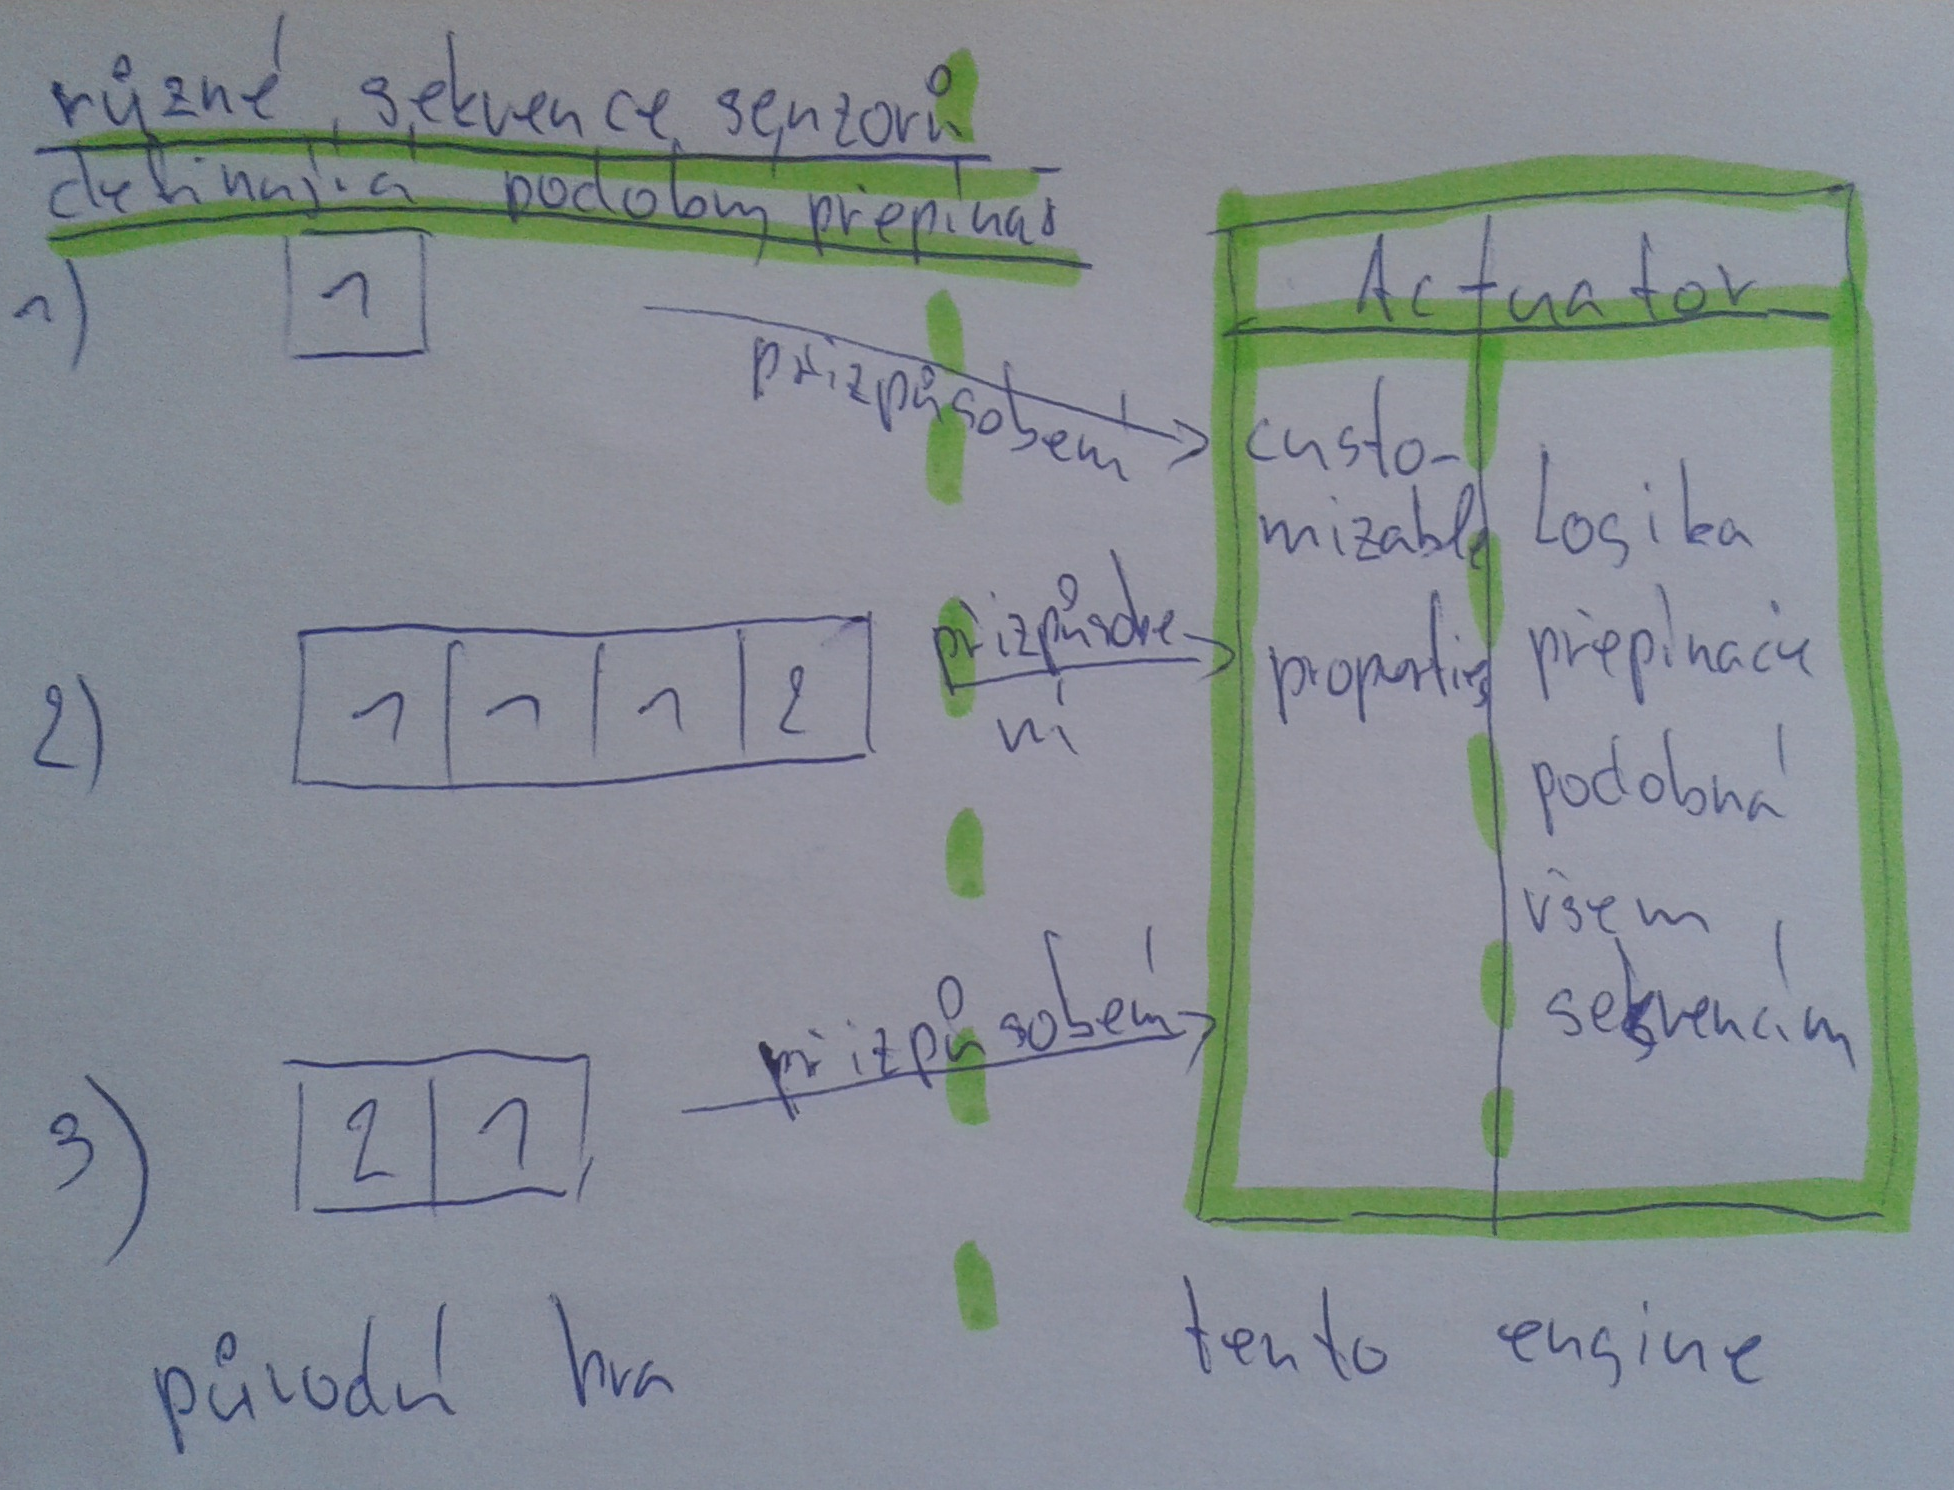
\includegraphics[width=\textwidth]{./img/actuator-object.png}
\caption{Ilustrace transformace sekvence senzorů na objekt přepínač.}
\label{actuator-object}
\end{figure}

Tento způsob sice řeší problém samotné reprezentace\vbref{actuator-representation}, ale později se ukázalo, že velice špatně. Například
kód převádějící sekvence na přepínače je složitý a nepřehledný. Bylo také složité vytvořit přepínač podle technické dokumentace\cite{TechnicalDocumentationFontanel05}
tak, aby fungoval opravdu správně. Popis v dokumentaci\cite{TechnicalDocumentationFontanel05} také asi není dostatečně přesný pro vytvoření tohoto úkolu.
I proto čím více přepínačů jsme tímto způsobem naimplmentovali, tím více se ukazovalo problémů. Nakonec jsme dospěli k závěru, že tento způsob reprezentace je nemožný.

\subsubsection{Druha reprezentace}

Tato reprezentace se snažila vyřešit problém nepřehlednosti\vbref{actuator-effective} kódu převádějícího sekvence na objekty přepínačů.
Proto je i zde použit typ objektu přepínač z první reprezentace v sekci \ref{rep-v1}. Parsování sekvence senzorů jsem se rozhodl udělat pomocí konečného 
automatu. Tedy tak, že pro každý objekt přepínače existovaly předdefinované sekvence senzorů. Konečný automat potom pomocí vstupní sekvence
identifikoval výsledný objekt přepínače. Při inicializaci objektu přepínače zde pak byla sekvence jasně definovaná, což řešilo problém s přehledností \vbref{actuator-effective}.
Později se nicméně ukázalo, že i malá změna v sekvenci senzorů může generovat podobný objekt. Takže by bylo třeba
spoustu předdefinovaných šablon, které se lišily ve drobnostech. Tím se ukázalo, že tento přístup není dostatečně obecný a nelze tedy použít. 

\subsubsection{Třetí reprezentace - výsledná}

Tato reprezentace se tedy oproti předchozím snažila přiblížit co nejvíce k systému použitém v enginu originální hry.
K dosažení tohoto cíle jsme se rozhodli použít dekompilované zdrojové kódy\cite{DMDecompilation} hry. Tím
je vyřešen problém nedostatečné dokumentace ve věci přepínačů\vbref{actuator-unclear}.

Vytvořili jsme tedy objekt přepínač, který má v sobě sekvenci senzorů, tak jako tomu je v originální hře.
Tím je vyřešen i problém nepřehlednosti převodního kód\vbref{actuator-effective}, jelikož jsou tyto reprezentace téměř identické.
S využitím zdrojových kódů jsme vytvořili odpovídající objektově orientovaný kód v jazyce C\#. Tato reprezentace
tak zajišťuje maximální korektnost implementace a přitom poskytuje možnost rozšíření - což je jedním z cílů\aref{aim-extensibility} této práce. 
Je tedy možné vytvořit nové senzory, které budou mít vlastní aktivační podmínky, a ty pak použít v přepínačích.
V originálním enginu je toto rozšiřovaní jen značně omezené, jednotlivé typy senzorů se tam odlišují jednobajtovým číselným identifikátorem.
Nicméně, jelikož jsme nechtěli rozšiřování enginu limitovat pouze na tento způsob vytváření senzorů, je si možné vytvořit přepínač, který
bude fungovat na úplně jiné bázi. Takže případné nové přepínače nemusí vůbec senzory používat. 

\subsection{Reprezentace zprávy přepínače}

Jak již bylo řečeno\vref{dungeon-objects}, celý systém mechanik herních úrovní je závislý na posílání zpráv. 
V originální hře je cíl odeslané zprávy vázán na souřadnice dlaždice, na kterou se má zpráva odeslat. 
Jelikož jsme se v enginu nechtěli vázat na tyto pevné souřadnice, rozhodli jsem se namísto nich
cílovou dlaždici identifikovat její referencí. To by případně ulehčilo práci při transformaci enginu tak, aby
dlaždice mohli mít více sousedů nebo aby nemusely být na pevné mřížce\vref{tile-representation}.
Při takovéto reprezentaci nicméně může nastává problém s inicializací dlaždic a přepínačů\vref{level-inicialization}.

V originální hře lze mezi dlaždicemi posílat pouze jeden typ zprávy. Jelikož cílem této práce je udělat engine
co nejrozšiřitelnější\aref{aim-extensibility}, engine poskytuje za určitých podmínek používat i jiné typy zpráv.
Těmito podmínkami jsou:
\begin{itemize}
\item Vlastní zprávy lze zasílat pouze vlastně vytvořením dlaždicím, které na daný typ zprávy musí být připraveny.
\item Všechny dlaždice musí umět přijímat originální typ zprávy - nicméně nemusí na ně reagovat.
\item Třída reprezentující vlastní zprávu musí být potomkem originální zprávy v hiearchii dědičnosti jazyka C\#.
\end{itemize}

\section{Reprezentace entit}

V originální hře existují pouze dva typy živých objektů, tj. nepřátelské entity a šampioni. Za účelem udělat engine
co nejrozšiřitelnější\aref{aim-extensibility} jsme se rozhodli pro živé objekty vytvořit následující abstrakci.  
Entitou je v tomto enginu každý objekt, s jehož vlastnostmi může interagovat nějaká akce\vref{action-combos}. Například akce
útok může entitu zranit nebo poškodit - pokud je neživá. Entity se dále dělí na živé a neživé. Příkladem v enginu použité neživé entity
jsou dveře, které je možné rozbít útokem. Živé entity tedy disponují následujícími vlastnostmi.

\begin{itemize}
\item vlastnosti - jsou to vlastnosti jako zdraví, odolnost,  atd. (viz sekce \ref{properties-skills}),
\item dovednosti - to ve výsledku znamená, že jsou schopny používat akce,
\item relaci vůči ostatním živým entitám - určuje, zda jsou vůči daným entitám přátelské či nepřátelské,
\item části těla a inventáře,
\item definují, jaké část dlaždic mohou zaujímat.
\end{itemize}

Každý z těchto bodů lze rozšířit, což může být užitečné v případě použití enginu pro implementaci jiné hry než Dungeon Master. 

\subsection{Vlastnosti}

V původní hře jsou vlastnosti šampionů\vref{properties-skills} a nepřátelských entit\vref{properties-creatures} pevně definované. 
Několik vlastností nepřátelských entit je odlišných od tě šampionových, nicméně ve většině se shodují.
S těmito odlišnostmi musí počítat akce, které modifikují vlastnosti entit. Pokud entita nějakou vlastností nedisponuje, je vrácena 
vlastnost se základní hodnotou. Například pokud provádíme akci útok magickou ohnivou koulí a entita nemá žádnou z vlastností
odolnost proti magii či odolnost proti ohni - jsou tyto vlastnosti v základním stavu. Útok akce tedy není v tomto případě
nijak modifikován. 

 \subsection{Dovednosti}

 Dovednosti šampionů jsou stejně jako jejich vlastnosti v originální hře pevně definovány\vref{properties-skills}. I v tomto bodě se nový engine snaží o větší
 dynamičnost. Opět platí, že každá entita nemusí mít všechny dovednosti. Pokud určitou dovednost entita nemá, vrátí se její hodnota s úrovní nula.
 V originální hře jsou dva typy dovedností a to základní a nebo skryté. Pokud některá akce vylepšuje skrytou dovednost
 rozdělí se získané zkušenosti mezi obě dovednosti\vref{properties-skills}. Tento koncept schopností není v enginu vyžadován a 
 záleží potom na konkrétní implementaci dovednosti. Konkrétní implementace také specifikuje množství zkušeností nutné pro 
 získání nových úrovní. Implementace dovedností pro hru Dungeon Master odpovídá implementaci nalezené ve zdrojových kódech hry.\cite{DMDecompilation}.

 \subsection{Relace mezi entitami}
 Další funkcí kterou oproti originálu engine umožňuje je definovat pro entity jejich nepřátelé. Každá živá entita má token identifikující
 skupinu. Entity v této skupině jsou mezi sebou přátelské. Každá entita si může nadefinovat svoje nepřátelské tokeny.
 Podle vzoru originálu jsou v hře pouze dva relační tokeny - první pro šampiony a druhý pro nepřátelské entity. Nicméně
 celý tento system je navržen právě pro stanovení obecnějších vztahů mezi entitami a to může být aplikováno v libovolném rozšíření hry.
 
\subsection{Tělo a inventáře}
Každá živá entita má definované její části těla. Oproti originálu, kde se řeší pouze části těla šampionů,
zde je možné definovat tělo pro každou entitu. Je tak možné pracovat s částmi těla entit, které nemají humanoidní formu.
Některé části těla se dají použít jako úložiště předmětů, ty potom mají nadefinováno s jakým typem úložiště jsou kompatibilní.
Tato reprezentace dává dobrý smysl. Například pokud máme lidskou část těla - nohy. A medvědí část těla - nohy. Tak lidské
kalhoty by měli jít nasadit pouze na lidské nohy, nikoliv medvědí. Naopak medvědí chrániče na nohy půjdou dát pouze na
nohy medvědí. Takto pokročilejší mechanismy v originální hře nejsou použity, předměty tam mohou sbírat pouze šampioni. Nicméně
při použití tohoto enginu k implementaci jiné hry jsou tyto mechanismy k dispozici. 

Předměty lze pak dále ukládat do dalších úložných prostorů.  O velikosti a typu těchto úložišť opět rozhoduje tvůrce konkretních 
entit. Nicméně stejně tak jako v originální hře, i tato instance má implementované 
úložiště pouze pro šampiony. Mezi taktové úložiště patří například batoh, kapsa, truhla, toulec atd.

\section{Reprezentace předmětů}

V herních úrovních jsou různě rozmístěné předměty, které lze sbírat a ukládat si je do inventářů šampionů.
Každý takový předmět náleží do nějaké kategorie(zbraň, lektvar, atd. - viz sekce \ref{grabable-items}). Každá
tato kategorie pak obsahuje několik typů předmětů. Pro každý typ předmětu pak existuje jednoznačný globální identifikátor\vref{item-descriptors}.
Identifikátory jsou použité například v přepínačích pro identifikaci typu předmětu, dle kterého se pak rozhodnou zda se aktivovat či nikoliv.
Platí tedy, že všechny instance daného typu předmětu mají stejný identifikátor.

Z počátku jsme pro stanovení identifikátorů zvolili stejnou strategii jako tvůrci originální hry, tedy každá
instance měla daný číselný identifikátor.
Nicméně takto zvolený způsob reprezentace identifikátorů by byl nepřehledný pro případné rozšiřitele, jelikož
by nemuselo být jasné, které identifikátory už jsou obsazené a které nikoliv. Dále v počátcích každá instance
předmětu měla všechny jeho vlastnosti a to i ty, které byl společné pro všechny instance daného typu\vref{item-descriptors}.

Pro splnění cíle \ref{aim-extensibility} teto práce bylo zapotřebí reprezentaci předmětů vylepšit.
Řešením problému bylo delegování společných vlastností předmětů do zvláštních tříd\cc{item-factories}, které odpovídají jednotlivým identifikátorům.
Tyto třídy navíc slouží jako továrny na předměty daného typu. Reference na konkrétní instanci třídy pak slouží jako identifikátor.
To ale znamená, že reference na tyto továrny jsou potřeba pro vytváření přepínačů. Z toho důvodu je součástí jádra enginu
objekt obsahující všechny továrny splňující tento vzor\vref{engine-core}.

\begin{figure}[H]\centering
\includegraphics[width=\textwidth]{./img/item-factories.png}
\caption{Ilustrace vztahu objektů a jejich továren.}
\label{item-factories}
\end{figure}

Každá továrna na předměty má také následující vlastnosti:
\begin{itemize}
\item hmotnost, 
\item jméno, 
\item kombo - definuje akce, které lze s předměty provádět,  
\item definice míst v inventáři, kam lze předmět uložit. 
\end{itemize}

\section{Reprezentace komb a akcí}
Každý typy akce definuje svoji továrnu, která je uložena v jádře enginu\vref{engine-core} - jako je tomu v případě předmětů.
Tyto továrny obsahují vlastnosti\vref{action-combos} o dané akci, které také určují požadavky pro provedení dané akce.
Pomocí továrny lze pak vytvořit samotný objekt reprezentující konkrétní danou akci, kterou lze následně vyvolat určitým 
směrem(sever, východ, jih, západ). Jak podmínky vytvoření akce, tak její provedení je naimplementováno dle dekompilovaných
zdrojových kódů\cite{DMDecompilation} originální hry. Každá továrna na předměty má potom specifikovaný seznam továren akcí,
které lze s předměty provádět.

\section{Reprezentace kouzel}
V jádře enginu jsou uloženy všechny symboly, včetně power symbolů\vref{magic-symbols}.
Tyto symboly mají definovány, kolik je třeba many pro jejich vyvolaní při daném power levelu.
Každé kouzlo potom definuje svoji továrnu, která je rovněž uložena v jádře enginu\vref{engine-core} - stejně jako je tomu v případě předmětů a akcí.
Objekt reprezentující kouzlo lze pak opět vytvořit pomocí jeho továrny. Pro vyvolání kouzla je potom třeba určit směr a entitu,
která kouzlo vyvolává. Chování vyvolávání a provádění kouzel je opět naimplementováno dle dekompilovaných
zdrojových kódů\cite{DMDecompilation} originální hry. Modifikace vlastnosti entity při vyvolávání symbolů
kouzla pak zajišťuje speciální manager. 

\section{Builder herních úrovní}

Aby bylo možné sestavovat herní úrovně z různých vstupní formátů\aref{aim-builders} bylo nutné tuto část vyčlenit do samostatného
objektu, který je pak předán jádru enginu\vref{engine-core-section}. Tento objekt budeme dále nazývat tzv. builder. Jádro enginu
pak po builderu vyžaduje vytvoření herních úrovní, přičemž mu předá sadu továren - který je rovněž uložen v jádře. Builder
by se měl také starat o kešování načtených úrovní, jelikož je engine po něm může požadovat několikrát. Objekt builderu
je předán jádru enginu při jeho vytváření, tímto způsobem je možné jádru předat vlastní implementaci builderu.

Tato práce obsahuje pouze jeden builder, který je schopný sestavit herní úrovně z datového objektu popsaném v sekci \ref{level-parsing}.
V sekci \ref{tile-representation} se došlo k závěru, že dlaždice zdí nebudou v tomto enginu existovat. Z toho důvodu jsme se 
v prvních fázích projektu rozhodli při vytváření herní úrovně procházet pouze dlaždice, které jsou od pozice hráče přístupné.
Toho bylo docíleno použitím algoritmu prohledávání do hloubky. Nicméně později se ukázalo, že některé nepřístupné části herní úrovně
jsou používané teleporty nebo přepínači. Z toho důvodu se od tohoto způsobu procházení dat dlaždic upustilo a nyní se procházejí 
postupně všechny dlaždice.

Pro transformování dat na objekty srozumitelné enginu se používají ještě další pomocné subbuildery\cc{sub-builders}. 
Samotné sestavování herní úrovně potom probíhá následovně. V cyklu jsou vytvářeny všechny dlaždice - přitom se za pomocí továren 
z jádra enginu provádí vytváření veškerých objektů, které dlaždice obsahuje.

\begin{figure}[H]\centering
\includegraphics[width=\textwidth]{./img/sub-builders.png}
\caption{Ilustrace struktury builderu.}
\label{sub-builders}
\end{figure}


\section{Inicializace objektů}\label{level-inicialization}

Tento projet si klade za cíl\aref{aim-extensibility} vytvořit co nejlepší objektový návrh. Jedním z faktorů, který by měl takový návrh
zahrnovat je, že veřejné budou jen nezbytně nutné položky tříd. Na to navazuje problém s inicializací takových tříd. 
Například přepínače potřebují referenci na cílovou dlaždici, ale zároveň jsou obsahem dlaždic, je tedy třeba oddělit fázi inicializace 
dlaždic od inicializace přepínačů. Nicméně potom nelze přepínače předat do dlaždic v konstruktoru a tím pádem je pro tuto akci třeba 
vytvořit veřejnou funkci nebo vlastnost, která tak provede. Tato funkce pak narušuje náš cíl, protože tuto funkci může kdokoliv
zvolat později, kdy už to není validní. Z toho důvodu jsme přišli s konceptem tzv. inicializátorů.

Inicializátor je datová třída obsahující vlastnosti, které by běžně byly parametry konstruktoru inicializovaného objektu.
Místo těchto parametrů je do konstruktoru předán inicializátor, který má také události vyvolané
při inicializaci a při dokončení inicializace. Třída beroucí inicializátor jako parametr konstruktoru se zaregistruje na tyto události a
tím pádem není nutná žádná přebytečná položka ve třídě pro inicializátor. Události jsou pak volané skrze metodu v inicializátoru.
Inicializátorem inicializovaná třída si z něj nakopíruje parametry a odhlásí událost. Od té chvíle už není možné třídu modifikovat.
Data inicializátoru se tedy mohou postupně naplňovat a po jejich naplnění se inicializace provede zavoláním jejich metody.
S využitím a asynchronních metod, je navíc možné vyvolat inicializaci prvku (např. přepínačů, které potřebují reference na dlaždice) 
již při vytváření dlaždic. Což vede k přehlednějšímu kódu a celkově k inicializaci cyklických struktur bez nutnosti přebytečných 
veřejných položek. 

S využitím dědičnosti inicializátorů je možné nasimulovat volání rutin konstruktorů, tak jak je v C\#  běžné. Na každé úrovní dědičnosti
se využijí některé vlastnosti inicializátoru. Nechť inicializátor B
je potomek inicializátoru A v hiearchii dědičnosti. A nechť C a D jsou třídy, které chceme inicializovat a zároveň D je potomkem C.
A také platí, že konstruktor třídy D vyžaduje inicializátor třídy B a konstruktor třídy C vyžaduje inicializátor A. potom inicializátor B můžeme
použít pro oba konstruktory tříd C i D. Přičemž na každé úrovni dědičnosti inicializátoru může být zvláštní inicializaci oznamující událost.
Pokud tedy inicializátor volá inicializační události ve správném pořadí, může to nasimulovat pořadí inicializace běžné u konstruktorů.
Při inicializaci dlaždic je právě tento způsob používán. Celou situaci znázorňuje obrázek \ref{initializer-inherence}.

\begin{figure}[H]\centering
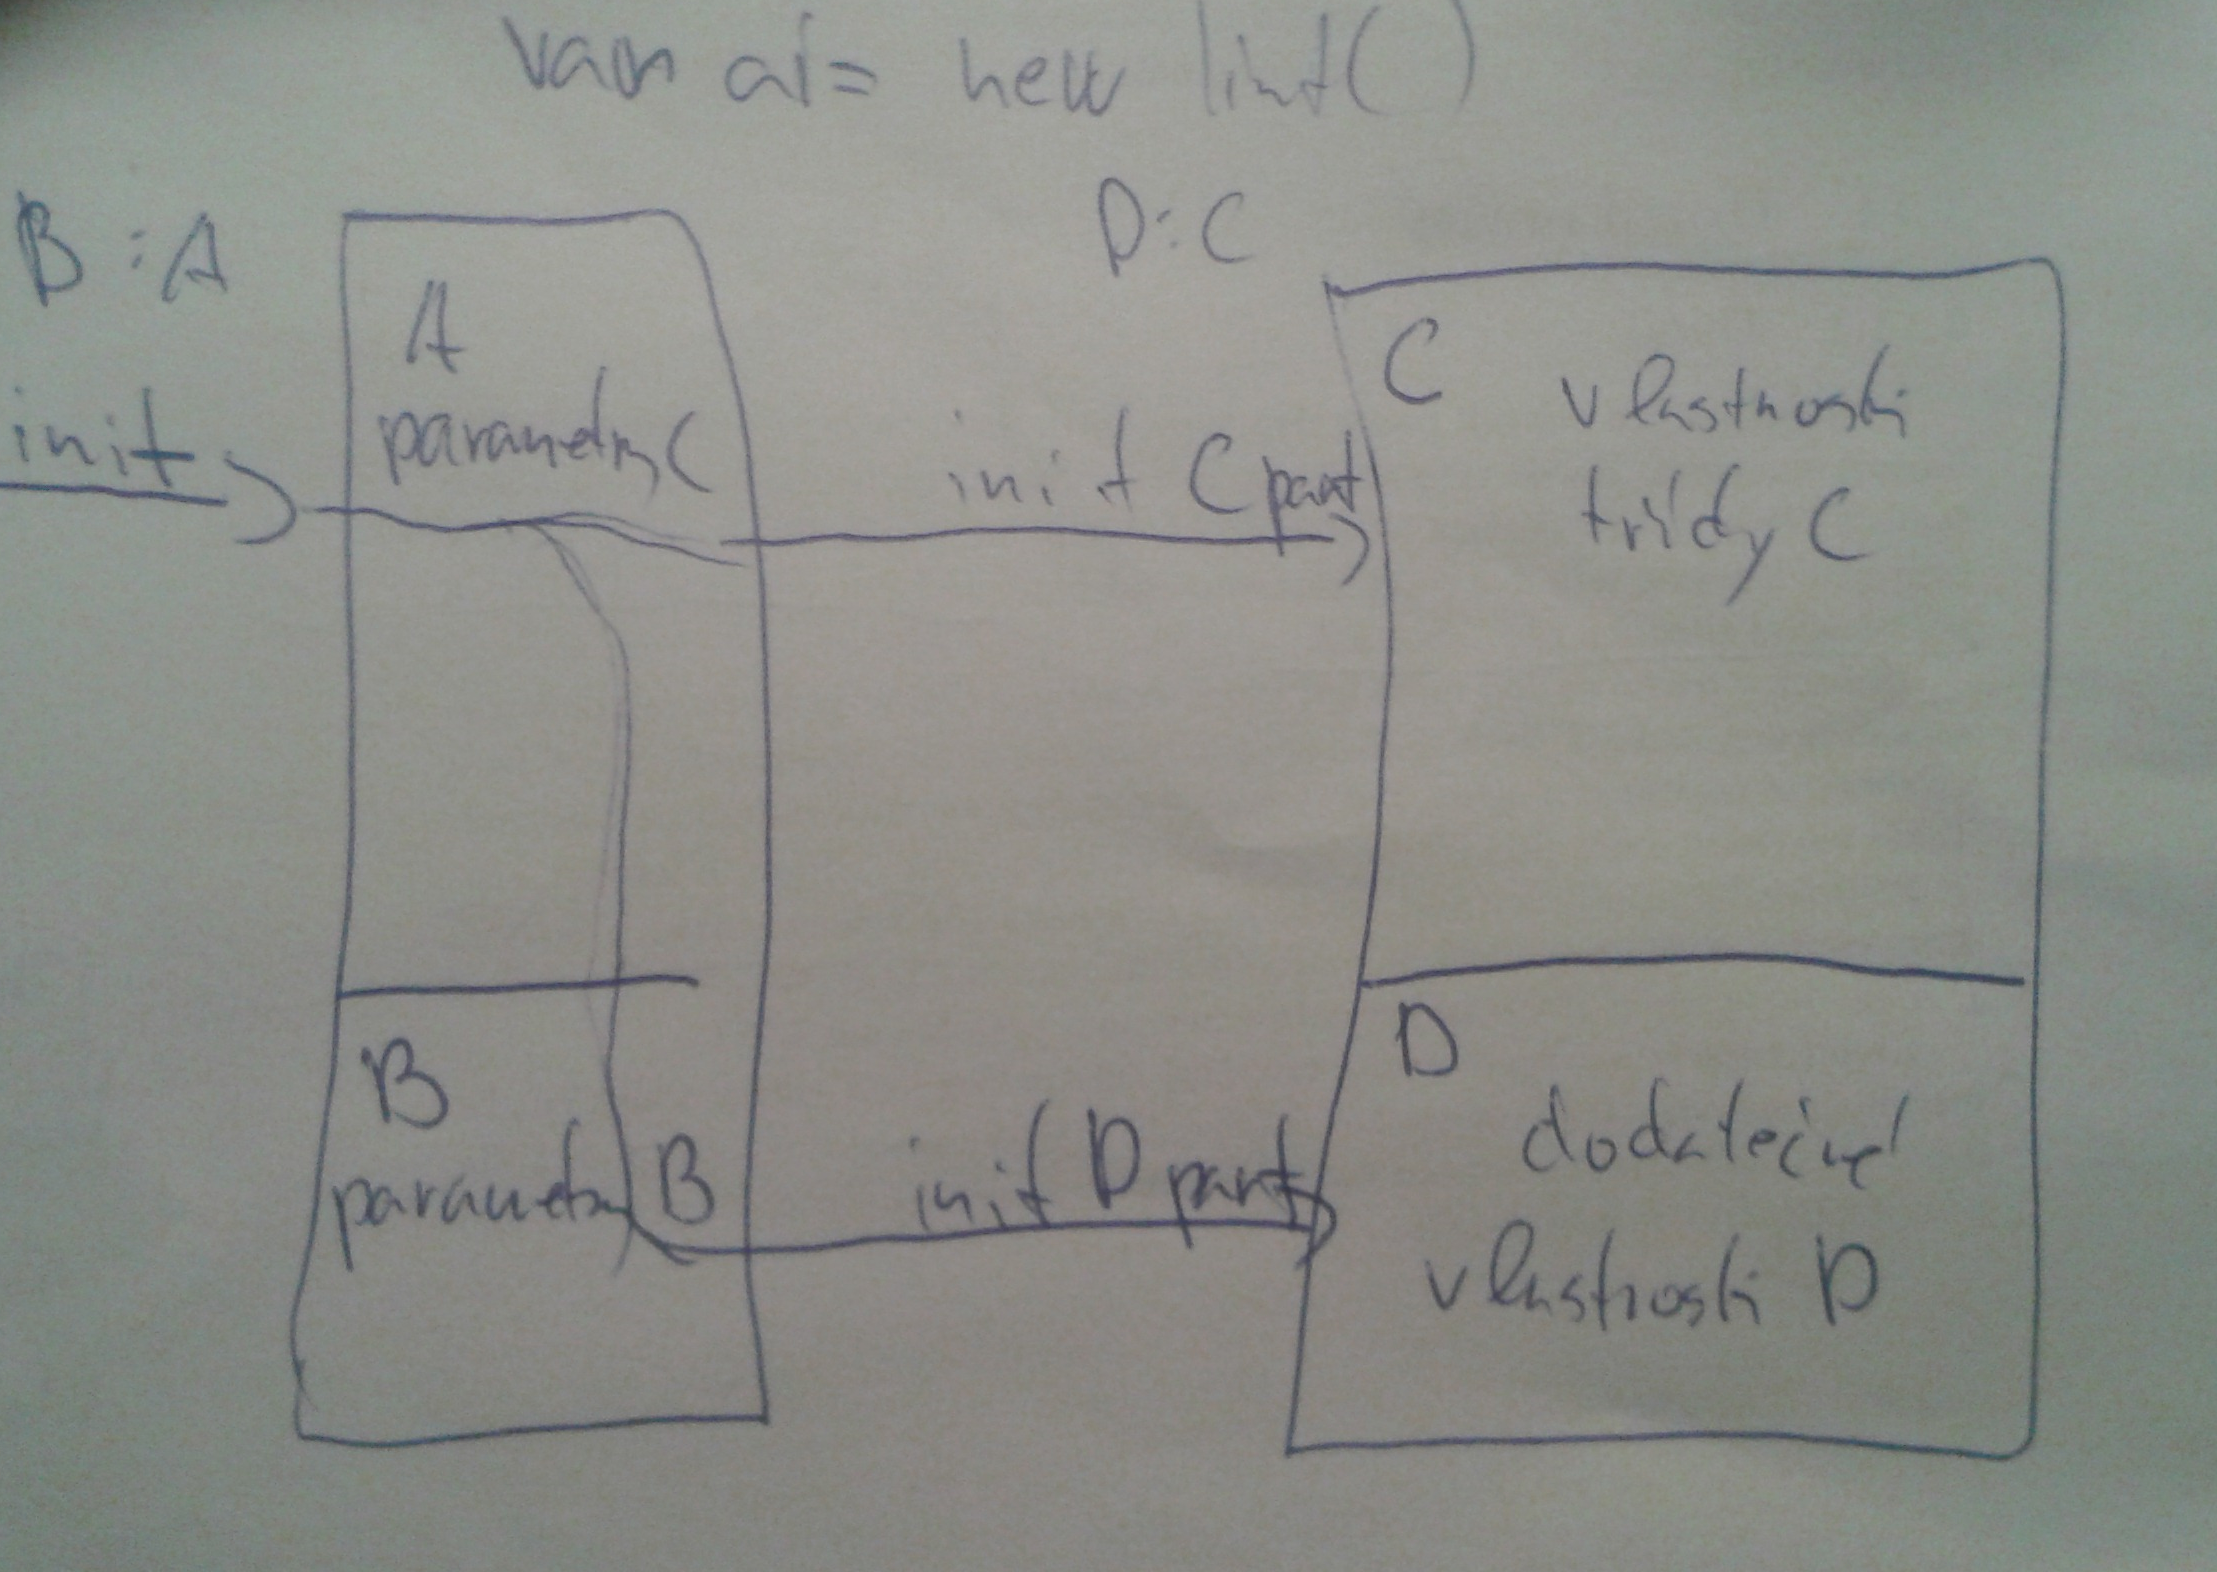
\includegraphics[width=\textwidth]{./img/initializer-inherence.png}
\caption{Ilustrace použití inicializátoru.}
\label{initializer-inherence}
\end{figure}

\section{Renderování a interakce}
Dalším cílem\aref{aim-rendering} tohoto projektu je oddělit v enginu zobrazovací vrstvu, tak aby ji bylo možné jednoduše nahradit za jinou.
Se zobrazovací vrstvou nicméně úzce souvisí jakým způsobem bude prováděna interakce s objekty, proto je v této vrstvě zahrnuta i ona. 
Každý objekt, který to vyžaduje má vytvořený vlastní renderer-interactor na míru. Jak renderer vypadá uvnitř je zpravidla na programátorovi. 
Nicméně obvyklý přístup je takový, že renderer má referenci na konkrétní renderovaný objekt. Podle jeho zpravidla readonly vlastnosti potom určuje
chování vykreslovaní nebo interakce. Pokud se jedná o renderery pro statické objekty(např. dlaždice), tak se zpravidla pozicování určuje relativně
vůči rodiči. Zobrazovací vrstva v tomto enginu nemá stejný grafický výstup jako originální hra, nicméně nic nebrání tomu napsat 
si tuto vrstvu tak, aby jí odpovídala.

\chapter{Vývojová dokumentace}
Následující sekce této kapitoly jsou určeny především pro lidi, kteří chtějí porozumět více celému enginu. Především
však dobře poslouží lidem, kteří by tento engine chtěli použít pro svoji hru nebo by chtěli jen rozšířit některé části
tohoto enginu Dungeon Masteru.

\section{Jádro enginu}
Jádro enginu tvoří třída \ccc{DungeonBase}, jak již bylo řečeno, stará se zejména renderování, aktualizování herních objektů,
inicializaci hráče, načítání a propojování herních map. Pokud má čtenář zájem o úpravu některých z těchto věcí, je tu správně.

\subsection{Renderovaní}
Tato sekce slouží pro čtenáře, kteří mají zájem o reimplementaci následujících věcí:

\begin{itemize}
\item Způsob výběru dlaždic, které se mají používat pro aktualizaci a rendering.
\item Pořadí v jakém se jednotlivé dlaždice renderují.
\item Použití osvětlení a celkově nastavení grafického zařízení.
\item Dosah viditelnosti
\item atp.
\end{itemize}

\subsubsection{Výběr a vykreslování použitých dlaždic}
V základní verzi vždy existuje kolekce právě používaných dlaždic. Tato kolekce se znovu naplní vždy, když hráč změní
pozici. dlaždice se zde vyhledávají algoritmem breath first search.

Vlastní algoritmus výběru dlaždic je možný přidat poděděním třídy \ccc{DungeonBase} a overridnutím  metody \ccc{UpdateVisibleTiles}. 
Metoda uloží do proměnné \ccc{currentVisibleTiles} vybraný seznam dlaždic. Tato proměnná je pak využívána v metodě \ccc{Draw}, kde se
ale renderují v opačném pořadí kvůli průhlednosti.


\subsubsection{Nastavení grafického zařízení}
Nastavení osvětlení a celkově efektu, textury a batcheru pro vykreslovaní minimapy, se provádí v metodě \ccc{InitializeGraphics}.
Jejím overridnutím je možné provést modifikace. Pokud nehodláte upravovat všechny popsané věci, je doporučené zavolat nejprve funkci rodiče
která data zinicializuje na základní hodnotu. Samotná minimapa se vykresluje funkcí \ccc{DrawMiniMap}, která se volá klasicky ve funkci 
\ccc{Draw}. Overridnutím této funkce je tedy možné například minimapu úplně odstranit, tak jako to je v originální hře. V této sekci je ještě
možná dobré zmínit proměnou \ccc{FogHorizont}, která je v základu používaná jednak jako maximální vzdálenost, po kterou jsou dlaždice hledány, a za druhé slouží v efektu jako 
hodnota FogHorizontu.

\subsection{Inicializace hráče}
O abstrakci různých způsobů načítaní levelů se stará interface \ccc{IDungeonBuilder}. Instanci implementace tohoto
rozhraní je nutné předa Dungeonu v konstruktoru. V základu se nové mapy načítají v momentu, kdy některá ze zobrazených
dlaždic je dlaždice navazující na další level. Takové dlaždice jsou právě dlaždice implementující  rozhraní  \ccc{ILevelConnector}.
Poslední tři levely získané skrze \ccc{IDungeonBuilder} jsou uložené v kolekci \ccc{ActiveLevels}. Pokud je nutné změnit 
strategii načítání levelů, je třeba overridovat metody \ccc{SetupLevelConnectors} popř. \ccc{ConnectLevels}. Pro změnu 
strategie ukládání a mazání aktivních levelů, je třeba podědit třídu \ccc{LevelCollection}. Kterou je pak nutno nastavit
do vlastnosti \ccc{ActiveLevels}. 

Následující sekce popisují jaké objekty lze jakým způsobem rozšířit či upravit. O tom jak takové nové objekty potom používat
pojednává pozdější sekce.

\section{Rozšiřitelnost dlaždic}
\subsection{Popis dlaždic}
Nejobecnější strukturu dlaždice definuje interface \ccc{ITile}. Dlaždice tedy musí obsahovat pozici vzhledem
k~mřížce dlaždic a potom level, ve kterém se nachází. Tyto vlastnosti používají příšery nebo hráč k~určení
své pozice. Dále obsahuje vlastnosti sloužící k rozhodovaní pohybu entit, předmětů a orientaci příšer. Další částí
je již zmiňovaný \ccc{LayoutManager}, který slouží k rozdělení prostoru mezi entitami na dlaždici. Podle něj se 
příšera či hráč rozhoduje, zda může na danou dlaždici vstoupit a obsadit, tak část jejího prostoru. Má také definované
soused, podle kterých se zase entity rozhodují při pohybu mezi dlaždicemi. Další část API slouží k modifikaci stavu dlaždice.
Stav jde buď přímo nastavit pomocí volaní odpovídajících funkcí nebo předáním zprávy. Poslední
část obsahuje metody a události pro vstup a odchod věcí z dlaždice. O volání těchto  funkcí se musí starat samy objekty,
které chtějí vstoupit či odejít. Takové objekty jsou poté skrze dlaždici aktualizovány, pokud implementují rozhraní
\ccc{IUpdateable}. To však již musí zařizovat jednotlivé implementace dlaždic, o niž bude řeč v další sekci.

\subsection{Inicializace dlaždic}
Jak již bylo zmíněno v analýze, k inicializaci dlaždic jsou použity tzv. inicializátory. Inicializátor
obsahuje vlastností, které by normálně byly předány jako parametry v konstruktoru. Ovšem v moment předávaní
inicializátoru do konstruktoru, inicializátor ještě nemusí být plný. Namísto toho má události \ccc{Initializing}
resp. \ccc{Initialized}, které jsou vyvolány při resp. po inicializaci. Na tuto událost je třeba zaregistrovat
inicializační funkci, která zkopíruje data z inicializátoru do samotného objektu. Pro každou úroveň hierarchie
dědičnosti jsou určeny zvláštní vlastnosti a zvláštní inicializační události. Rodičovské události  inicializátoru jsou vždy
po zdědění rodičovského inicializátory zakryty novými inicializačními událostmi pro danou proveň dědičnosti.
Tento způsob je použit pouze pro inicializaci dlaždic. Pro jiné objekty, může inicializátor sloužit pouze jako 
objekt udržující parametry. Parametry, které jsou hned v konstruktoru inicializované. To vše záleží na konvice kterou si
programátor zvolí.

\subsection{Implementace dlaždic}
O částečnou implementaci rozhraní \ccc{ITile} se stará třída \ccc{Tile}. Definuje základní layout manager,
nicméně je ho popřípadě možné overridovat vlastní implementaci. Zejména se pak ale stará o inicializaci 
pozic na mřížce, levelu a sousedů skrze \ccc{TileInicializator}. Dále abstraktně deklaruje vlastnost
\ccc{SubItems}, na jejichž objektech, které implementují \ccc{IUpdateable} volá metodu \ccc{Update} skrze
metodu \ccc{Update} na dlaždici. Abstraktně deklaruje také vlastnosti \ccc{Sides}, kde těmto stranám přeposílá 
případné zprávy, které přišli na tuto dlaždici skrze metodu \ccc{AcceptMessageBase}. Dále implementuje
také funkce pro vstup/odchod objektů tím, že vyvolá odpovídající události na dlaždici. Pokud tedy chcete
volání těchto událostí zachovat, je při případném overridování metod nutné zavolat implementaci rodiče. Všechny
předchozí popsané funkce je možné overridovat v potomkovi a tak přizpůsobit prováděné akce.

Přímý generický potomek \ccc{Tile\textlangle TMessage\textrangle} poskytuje již zmiňovanou možnost přijímat
v potomcích vlastní zprávy. Poděděním tohoto typu, specifikováním typu zprávy v typovém parametru a následnou implementací metody 
\ccc{AcceptMessage} lze definovat rutinu při příjmu zprávy. Tato třída overriduje a zároveň uzavírá metodu rodič \ccc{AcceptMessageBase},
která deleguje zprávy typu \ccc{TMessage} do metody \ccc{AcceptMessage}. Naopak základní implementace metody \ccc{AcceptMessage}
je zavolání právě rodičovské implementace \ccc{AcceptMessageBase}. Takže při případném overridování této funkce
stojí za zamyšlení, zda-li  je třeba volat implementaci rodiče či nikoliv. Všechny dlaždice, které dědí ze třídy
popsané v tomto odstavci vytváří potomky dva. Jednoho pro případně rozšiřitele, která ponechává 
typový parametr.A druhá, která definuje typový parametr na obecný typ \ccc{Message}. Ještě stojí z zmínku,
že každá zpráva musí dědit právě ze třídy \ccc{Message}.

\subsubsection{Dlaždice podlaha}
Za zmínku ještě stojí přímý potomek třídy \ccc{FloorTile\textlangle TMessage\textrangle} a 
to \ccc{FloorTile\textlangle TMessage\textrangle}.  Tato třída se stará jak o interakce, tak rendering
zdi a podlahy. Stará se tady například o možnost pokládaní předmětů na zem, či u zdí do případných výklenků. 
Dále se stará  o zobrazování a aktivování případných přepínačů. Z toho důvodu, pokud se chystáte
vytvářet nějakou novou dlaždici, je dobré se zamyslet, jestli  nevyužít již tuto implementaci. Nicméně nic
nebrání tomu podědit přímo z \ccc{Tile\textlangle TMessage\textrangle}, pokud by tato implementace z
nějakého důvodu nevyhovovala. Při drobných úpravách je zase možné třídě podstrčit pozměněné-poděděné implementace 
jejich stran, ať už zdí nebo podlahy. Třída deleguje veškeré akce vstupu/odchodu do samotné podlahy
typu \ccc{FloorSide}. Stejně tak implementace kolekce  \ccc{SubItems} se deleguje na podlahu.

\subsubsection{Další dlaždice}
Další dlaždice již převážně využívají dědičností právě již zmíněnou předchozí podlahu. Výjimkou jsou například schody.
Schody jsou příkladem  dlaždice, který implementuje rozhraní  \ccc{ILevelConnector},  které požaduje implementaci 
následujících vlastností
\begin{itemize}
\item cílový level
\item pozice cílové dlaždice v cílovém levelu
\end{itemize}

Jak už bylo zmíněno engine potom při načtení levelu nastaví poslední položku tohoto interface 
\ccc{NextLevelEnter} na odpovídající dlaždici. A je už na samotné dlaždici, aby při změně této vlastnosti udělala 
potřebné akce. U schodů je to například nastavení sousedů vedoucích do dalšího levelu. Právě zde se například hodí 
overridování vlastnosti \ccc{Neighbors} vlastní třídou starající se o sousedy. Tato možnost je použita ještě u jámy,
kvůli propadu do nižšího levelu. Rozhraní spojující levely je pak ještě u teleportu, kde při vstupu na teleportační
dlaždici a splnění požadavku teleportu se tento objekt teleportuje na jinou dlaždici. Za zmínku ještě stojí existence
rozhraní \ccc{IHasEntity}, které obsahuje vlastnost typu entity. Implementuje ho například dlaždice typu dveře,
která vrací jako entity dveře. Tímto způsobe lze pak například útokem dveře rozbít, protože jsou definované jako 
entita s vlastností zdraví, odolnost atp. Nikde jinde v enginu toto využito není, tím více prostoru mají případní
rozšiřité.

\subsection{Strany dlaždic}
Jak již bylo naznačeno v předchozích sekcích, dlaždice mohou mít strany. To mohou být ať už zdi, tak i podlaha nebo strop.
Každou tuto stranu reprezentuje samostatný objekt, který má samostatný renderer-interactor. Poděděním z těchto hotových tříd
si lze tedy ušetřit nějakou práci. Není to však nutnost, je možné si pro své dlaždice implementovat vlastní
strany implementací rozhraní \ccc{ITileSide}. Toto rozhraní vyžaduje pouze položku pro renderer a z kompatibilních důvodů
pro starou verzi požaduje, aby byla schopna přijímat zprávy \ccc{Message}.

\subsubsection{Jednotlivé implementace}
Třída \ccc{TileSide} slouží jako rodič všech zdí implementovaných ve hře. Nereaguje nijak na interakci
hráče a její renderer pouze renderuje zdi  texturu na správné místo, popř. dekoraci.

Jejím přímým potomkem je třída \ccc{ActuatorTileRenderer},ta navíc obsahuje přepínač a její renderer se navíc
stará o jeho vykreslování a interakci.

Dalším potomkem je třída \ccc{TextTileSide}, jejíž renderer navíc zobrazuje na zdi text, v závislosti na tom,
zda-li je viditelný. Viditelnost textu lze změnit zasláním zprávy s odpovídajícími informacemi této straně.

Předposlední a nejsložitější stranou je třída  \ccc{FloorTileSide}.  Tato strana obsahuje čtyři úložiště na předměty,
kam je může uživatel pokládat. Je to jedno z míst, kde je potřeba komunikovat s rodičovskou dlaždicí, k tomu
slouží událost \ccc{SubItemsChanged}, která se vyvolá vždy, když byl nějaký předmět odebrán nebo přidán.
Pomocí enumerátoru tohoto objektu je potom možné vyenumerovat obsažené věci. Předměty lze pak na podlahu přidávat dvěma 
způsoby, jednak přímo z ruky hráče pomocí renderer-interactoru do úložného prostoru na podlaze. Toto
přidání opět pomocí události informuje přes podlahu rodičovskou dlaždici. Další způsob je zavolání metody 
\ccc{OnObjectEnter} resp. \ccc{OnObjectLeft},  které také vyvolají notifikační událost o změně a přidají objekt do nějakého prostoru.
Tento způsob je použit například u teleportu, kde se vědci přidávají do dané dlaždice voláním metody \ccc{OnObjectEnter}.
Tato metoda pak volá odpovídající metodu podlahy. Poslední stranou je  třída \ccc{ActuatorFloorTileSide}, která pouze navíc přidává 
nášlapný přepínač.

\section{Renderery}
Jelikož každá dlaždice a každé strany dlaždic mají renderery, je jím čas věnovat tuto sekci. Všechny tyto objekty
a mnoho dalších k tomuto účelu implementují rozhraní \ccc{IRenderable}, které pouze vyžaduje  položku typu \ccc{IRenderer}. 
Stěžejní funkce tohoto rozhraní jsou funkce \ccc{Render} a \ccc{Interact}. 

Nejdůležitější z parametrů těchto funkcí je dosavadní transformace. Tj. obsahuje složeninu transformací složenou z jednotlivých
transformací na cestě z kořene stromu reprezentující závislosti renderer na sobě. Takže například kořen strumu bude renderer
dlaždice, jeho syn bude strana dlaždice, její syn bude výklenek ve zdi a její syn bude předmět ve
výklenku(list). Při takovéto reprezentaci se pak musí všechny renderované objekty posunout či jinak transformovat vůči jejich rodiči.
Tzn. každý renderer si musí zvolit pozicovací konvenci, kterou pak musí závislé renderery dodržovat. Tento způsob renderování je požíván u statických objektu jako
jsou dlaždice, zdi, výklenky a podobně. Pro pohybující objekty je používaná absolutní pozice a renderery
těchto objektů transformují objekty přímo na jejich pozici. Volba mezi těmito dvěma případy je na programátorovi.

Renderery jsou vždy dělány na míru objektu, který mají renderovat. Tzn. často se renderer v konstruktoru 
inicializuje instancí s konkretním typem. Třída této instance pak má zpravidla readonly vlastnosti,
podle kterých renderer určuje, co má vykreslovat. Jelikož implementovaná grafická vrstva je pouze ve formě proof of concept,
je co nejjednodušší a neobsahuje například animace. Nicméně ze zde popsané povahy renderer je jasné, že 
toho může být dosaženo vytvořením událostí na renderovaných objektech, které si renderer zaregistruje.
Dovedu si představit, že by šla s takovýmto návrhem velmi jednoduše udělat grafická vrstva, která bude
velmi pěkná, bude mít kvalitní šD modely animace. Zabralo by to jen spoustu času a byla by k tom u potřeba horda grafiků.

Při podědění nějakého rendereru je třeba zjistit dosavadní transformaci, která je normálně vypočítána v rodiči.
K tomuto záměru slouží funkce \ccc{GetCurrentTransformation}, která bere jako parametr dosavadní transformaci.
Poděděním jež existujícího rendereru lze ušetřit mnoho práce a opakujícího se kódu. Proto je takový přístup v této implementaci často použit.
Funkce popsané na začátku sekce jsou samozřejmě virtuální a jdou overridovat,
obsahují taky jeden parametr typu \ccc{object} pro případné předávaní dodatečných dat mezi renderery. Tohoto parametru není nikde v této implementaci využito.

Jelikož renderery zásadně mění vzhled a pozici všech věcí, je nutné tuto vrstvu propojit i s interakcí.
Interakční funkce má skrze parametr typu \ccc{ILeader}  přístup k položce interactor, která je typu \ccc{object}.
Daný renderer musí vědět, pro jaký typ interactoru je a na ten si ho musí vhodně přetypovat. V této implementaci je použit paprsek (\ccc{Ray}). 
Celý tento koncept interactoru by šel sice udělat genericky, ale prolínal by se celou strukturou rendererů a z toho
důvodu jsem se rozhodl v tomto místě ustoupit. A udělat situaci jednoduší na úkor kontroly za překladu.


\section{Přepínače}
\subsection{Úvod}
Jak již bylo řečeno, přepínače se skládají z jednotlivých senzorů. Senzory pak mohou provádět následující akce:

\begin{itemize}
\item změna stavu  dlaždice
\item proházení senzorů přepínače
\item přidání zkušeností hráči
\end{itemize}

Senzory mohou být aktivovány:

\begin{itemize}
\item Kliknutím na dekoraci senzoru, pokud je senzor na zdi a je to poslední senzor přepínače.
\item Zprávou od vyslanou jiným senzorem.
\end{itemize}
Tento typ přepínačů odpovídá přepínačům v původní hře.

Dále engine povoluje nové přepínače, který nemusí používat senzory. Je tedy čistě na programátorovi, jakým 
způsobem se bude přepínač aktivovat. 

\subsection{Implementace přepínačů se senzory}
Za přepínačem stojí navenek interface \ccc{IActuatorX}. Toto rozhraní pouze vyžaduje API pro příjem 
zpráv typu  \ccc{Message} pro dodržení kompatibility s původní hrou. Jelikož ostatní aktivace záleží
na typu přepínače. Protože například nášlapný přepínač se aktivuje jiným způsobem než přepínač na zdi.

\subsubsection{Implementace senzorů}
Senzory provádějí samotné akce přepínačů popsané v úvodu. Odpovídající akce jsou provedeny pouze pokud
byl daný senzor aktivován. Po kliknutí na přepínač, dojde postupně u všech senzorů o pokus jejich aktivace.
Každý typ senzoru má jinou podmínku aktivace. Senzory se dělí na senzory použité na podlaze,  na zdi a
na speciální tzv. logické senzory.

Hlavní třídou reprezentující přepínač je třída \ccc{SensorX}. Tato třída obsahuje některé společné funkce,
které může využít každý potomek. Dále take definuje vlastnosti, které lze rozdělit do tří skupin.
Tyto vlastnosti jsou inicializovány inicializátorem, který slouží pouze jako datový nosič. Jde o inicializátor
typu \ccc{SensorInitializerX}. Pro použití v potomcích se můžou použít poděděné verze tohoto inicializátoru.
Následuje seznam vlastností.

Obecné vlastnosti:
\begin{itemize}
\item Opoždění akce - čas v milisekundách, po kterém se provede případná akce 
\item Informace, zda-li je efekt určen lokálně pro rodičovskou dlaždici, či pro nějakou jinou.
\item Flag opakovatelnost - každý senzor ji používá trochu jinak, ale většinou pokud je true, tak se obrátí cílová akce
\item Na jedno použití - senzor se po první aktivaci zablokuje, a není dále používán.
\item Flag určující, zda po aktivaci dojde k přehrání zvuku. (v tomto enginu není použit)
\end{itemize}

Vlastnosti pro lokální akci:
\begin{itemize}
\item Flag určující, zda-li se má seznam senzorů při aktivaci zarotovat.
\item Flag určující, zda-li se mají hráči po aktivaci přidat zkušenosti.
\end{itemize}

Vlastnosti pro vzdálenou akci:
\begin{itemize}
\item Efekt - Určuje jaký efekt má odeslaná zpráva po aktivaci. (Akce může být obrácená pomocí flagu popsaného v obecných vlastnostech)
	Hodnoty efektu jsou následující:
	\begin{itemize}
	\item Aktivace 
	\item Deaktivace
	\item Přepnutí stavu
	\item Drž - Tento stav nelze odeslat ve zprávě a je na senzoru, aby ho interpretoval pomocí aktivace či deaktivace.
	\end{itemize}
\item Směr použitý v odeslané zprávě. Směr může být interpretován jako číslo. (Lze získat pomocí \ccc{MapDirection.Index})
\item Reference na cílovou dlaždici.
\end{itemize}

Kromě předchozích vlastností obsahuje tato třída funkce pro vykonání akcí senzorů. Funkce  \ccc{TriggerEffect} odešle zprávu 
podle vlastností senzoru na danou pozici, pokud je cíl vzdálený. Jinak provede akci pro lokální efekt. Lokální efekt lze 
také vykonat přímo zavoláním funkce \ccc{TriggerLocalEffect}. Tyto funkce lze použít pouze v potomcích.

Dále se senzory dělí na senzory použité na zemi resp. na zdi. Tomu odpovídají třídy  \ccc{FloorSensor} a \ccc{WallSensor}.
Obě tyto třídy mají funkci \ccc{TryTrigger}, která se stará o provedení případného efektu. Zda-li se efekt provede stanoví
funkce \ccc{TryInteract}. Pro každou variantu mají funkce odlišné parametry. Pokud tedy chcete vytvořit vlastní senzor,
implementujte funkci \ccc{TryInteract}. Tato funkce bude volána z funkce \ccc{TryTrigger} a bude tedy dělat obecnou funkcionalitu 
odeslání zprávy a určení výsledného efektu zprávy. Pokud chcete změnit i tuto funkcionalitu, poskytněte vlastní implementaci 
i pro tuto funkci.

Kromě předchozích senzorů ještě existují tzv. logické senzory. První z nich je \ccc{LogicGateSensor}, který funguje 
jako logické hradlo. Celkem má k dispozici osm bitů. Čtyři  nich jsou nastaveny na nějaké hodnoty a ostatní na nuly. 
S druhou čtveřicí lze manipulovat pomocí zpráv. Index směru zprávy určuje kolikátý bit se má ovlivnit. A tento bit
je pak ovlivněn akcí zprávy. Pokud se pak stane, že jsou obě čtveřice stejné, je vyvolaný efekt senzoru. Dalším
senzorem je \ccc{CounterSensor}, který má dané číslo. Aktivační zprávy toto číslo poté navyšují a deaktivační zprávy
ho snižují. Pokud je číslo  nula, je vyvolaný efekt.
 

\subsubsection{Implementace přepínačů používající senzory}
Rodiče všech přepínačů kompatibilních originální hře tvoří třída \ccc{Actuator}. Tato třída poskytuje
pouze společnou rutinu pro zarotování senzory přepínače. Lze vyvolat pouze z potomků. Zda-li se mají
senzory zarotovat určuje dle vlastnosti  \ccc{Rotate}, která se poté nastaví na false. Tato funkce se
volá z potomků pokud proběhl pokus o aktivaci nějakého senzoru.

Prvním potomkem předchozí třídy je třída \ccc{FloorActuator}, která může obsahovat pouze senzory určené
na podlahu tj. \ccc{FloorSensor}. Pokus o její aktivaci se provádí funkcí \ccc{Trigger}. Jako první parametr se jí předává objekt,
který vstupuje/odchází z dlaždice. Potom seznam všech objektů na dlaždici a naposled informace zda objekt
vstupuje či vystupuje. Pro přepínač je vytvořena speciální podlaha \ccc{ActuatorFloorSide}, která se stará 
o volání zmíněné funkce.

Dalším potomkem je třída \ccc{WallActuator}, která může obdobně obsahovat pouze senzory určené na zeď tj. \ccc{FloorSensor}.
Pokus o její aktivaci se provádí opět funkcí \ccc{Trigger}, která bere jediný parametr typu \ccc{ILeader}. Pro přepínač
již není vytvořena žádná speciální strana dlaždice, ale je použita strana přijímající obecné přepínače \ccc{ActuatorWallTileSide}.
Funkce \ccc{Trigger} je pak volána skrze renderer dané strany.

Poslední speciální implementací je třída \ccc{LogicActuator}, která může obsahovat již zmíněné logické senzory.
O komunikaci s jejími senzory se stará rodič, pomocí zasílání zpráv. Pro tento přepínač je vytvořená speciální dlaždice, která není 
odnikud přístupná. Tato dlaždice je reprezentovaná třídou \ccc{LogicTile}. 

\subsection{Implementace obecných přepínačů}
Tato sekce pojednává přepínačích, které ke své funkci nepoužívají senzory. Jejich vznik byl podnícen snahou, dát
programátorovi větší svobodu při tvorbě přepínačů, nicméně zároveň řeší následující problém. Kromě standardních
dekorací v se v dungeonu vyskytují dekorace, které provádějí nějakou funkci po kliknutí na ně. K těmto dekoracím však v originální
hře nenáleží žádné senzory. Jedná se o tzv. náhodné dekorace, kdy každá zeď má definováno, zda může obsahovat náhodné dekorace.
Při generování mapy se pak s určitou pravděpodobností dekorace na zeď dá či nikoliv. Z toho důvodu tento engine
neobsahuje stejné dekorace na stejných místech, protože není znám náhodný generátor k tomu použitý. Nicméně zpět 
k problému akcí po kliknutí na dekoraci. Studii dekompilovaného kódu originální hry  (viz.\cite{DMDecompilation}) se ukázalo,
že některé akce jsou fixovány na konkrétní typy dekorací. Takže například v dekorace s výklenky mají napevno implementovaný 
kód umožnující vkládaní předmětů do výklenku. Dalším příkladem jsou fontánky, které naplňují lahve s vodou. Posledním příkladem
speciální dekorace je Vi Altair výklenek, který dokáže po vložení kostí oživit šampiona. Jelikož tyto dekorace
mohou být i součástí senzorů, bylo zapotřebí udělat kolem samotných dekorací wrapery, které zajišťují případné akce.
Tyto wrapery jsou tedy implementací přepínačů tj. rozhraní \ccc{IActuatorX}, kdy dekorace bez akce neprovádějí žádnou akci a dekorace s nějakou akcí
danou akci provádějí. O samotné vyvolání interakce se opět musí postarat renderery. Takže zmiňované senzory jsou vlastně přepínače v přepínačích. 

Obecné přepinače tedy nemají nikterak napevno zvolený formát, je čistě na programátorovi, jak implementuje uvnitř jejich funkci a 
jakým způsobem bude s přepínači prováděna interakce. Existující implementace tedy jsou \ccc{DecorationItem}, která
neprovádí žádnou interakci, ale pouze rendering o který se stará \ccc{DecorationRenderer}. Dále jde o třídu \ccc{Alcove},
která reprezentuje výklenek a má odpovídající \ccc{AlcoveRenderer}. A poslední z nich je \ccc{ViAltairAlcove}, který dědí
ze třídy \ccc{Alcove} a stará se o již zmiňovanou reinkarnaci šampionů.
 
\section{Herní entity}
Za deklarací neživých entit stojí rozhraní \ccc{IEntity}. Definuje pouze funkci pro získání vlastnosti dané entity.
Za živými entitami stojí naopak rozhraní \ccc{ILiveEntity}, která navíc disponuje funkcí pro získání schopností. Dále
deklaruje:

\begin{itemize}
\item tělo entity
\item způsob rozmístění entity na dlaždici
\item relace s dalšími entitami
\end{itemize}

\subsection{Implementace vlastností entit}
Vlastnost deklaruje rozhraní \ccc{IProperty}. Nejprve obsahuje vlastnost \ccc{Value}, která stanovuje nynější hodnotu
dané vlastnosti. Tato hodnota je jako jediná možná měnit z venčí. V jejím getteru a setteru se typicky provádějí kontroly okrajových hodnot a případné reakce na ně. 
Další vlastností je \ccc{BaseValue}, což je nejvyšší hodnota, které může vlastnost nabýt, pokud není nějak modifikovaná.
Maximální hodnotu včetně modifikací určuje vlastnost \ccc{MaxValue}. Poslední vlastností je \ccc{AdditionalValues}, která shromažďuje
právě dané modifikace. Je to sekvence typu \ccc{IEntityPropertyEffect}, která definuje hodnotu a typ hodnoty. Poslední
vlastností je již zmíněný typ vlastnosti. Jednotlivé typy vlastností jsou definovány jako reference na třídy implementující
rozhraní IPropertyFactory. Entita na základě tohoto typu potom vrací příslušné vlastnosti. Typem může být jakákoliv 
třída implementující toto rozhraní, nicméně typická taková třída nemá žádné položky.
Proto existuje generická třída \ccc{PropertyFactory}, která bere jako typový parametr právě typ alespoň \ccc{IProperty}.
Tato třída se řídí vzorem singleton, jejíž jediná instance lze získat přes statickou položkou \ccc{Instance}. Takto lze pak 
generovat typy pomocí samotné třídy reprezentující vlastnosti, takže není nutné deklarovat stále nové třídy, které nic nedělají.

Za zmínku ještě stojí částečná implementace rozhraní \ccc{IProperty} a to třída \ccc{Property}. Tato třída definuje 
maximální hodnotu jako součet základních hodnoty a sumu modifikujících hodnot. Dále Při nastavení konkrétní hodnoty ořezává
hodnotu do povoleného intervalu to je mezi nulou a maximální hodnotou. Také definuje událost vyvolanou při změně hodnoty.
 A naposledy definuje kolekci modifikujících hodnot jako \ccc{HashSet\textlangle T\textrangle}. Všechny vlastnosti 
 jsou deklarovány abstraktně nebo virtuálně. Tato třída lze použít k usnadnění implementace vlastností.

 Některé vlastnosti mohou požadovat přístup k jiným vlastnostem či přístup k samotné rodičovské entitě. V takovém
 případě je čistě na programátorovi, jak takového cíle dosáhne. Typicky se v takovém případě předá v konstruktoru
 potřebná vlastnost nebo se vytvoří událost, která danou závislost deleguje vně. 

 Seznam předdefinovaných vlastností je možné najít ve jemném prostoru \ccc{DungeonMasterEngine.DungeonContent.Entity.Properties}.
 Jak již bylo zmíněno, může nastat, že daná entita vlastnost neobsahuje. V takovém případě je dobré kvůli dodržení konzistentnosti
vracet předdefinovanou instanci  třídy \ccc{EmptyProperty}. Nicméně rozhodně to není povinností při všech použití enginu.

\subsection{Implementace schopností entit}
Schopnosti deklaruje rozhraní \ccc{ISkill}. První vlastností tohoto rozhraní je \ccc{SkillLevel}, která udává úroveň,
na které je daná schopnost. Do této hodnoty jsou započítány i úrovně získané například kouzelnými předměty. Hodnotu
bez těchto extra úrovní určuje vlastnost \ccc{BaseSkillLevel}. Dále obsahuje vlastnosti \ccc{Experience} a \ccc{TemporaryExperience}
určující dosavadní hodnotu zkušeností. Dále obsahuje vlastnost \ccc{BaseSkill}, což je reference na základní(viz. analýza) schopnost. Pokud
je daná schopnost již základní, je hodnota \ccc{null}. Přidat schopnosti zkušenosti je možné zavoláním funkce \ccc{AddExperience}.
Konkrétní algoritmus přepočítávání zkušeností na levely záleží vždy  na konkrétní implementaci. Stejně jako u vlastností 
i zde existuje vlastnost \ccc{Type}, tentokrát ale typu \ccc{ISkillFactory}. Stejně jako u vlastností, je možné tyto reprezentanty
vytvářet pomocí generické třídy \ccc{SkillFactory}. 

Třída \ccc{SkillBase} implementuje získávání zkušeností schopností jako v originální hře. Všechny schopnosti 
využívající tuto třídu jsou ve jemném prostoru \ccc{DungeonMasterEngine.DungeonContent.Entity.Skill}. Stejně jako
u vlastností i zde entita nemusí mít dotazovanou schopnost. V takovém případě vrací instanci třídy \ccc{EmptySkill}.

\subsection{Tělo a inventáře entity}
Následující API umožňuje vytvořit různé druhy těl pro různé entity. Každá část těla může sloužit jako úložiště. Dále pak existují externí
úložiště. API je natrhnuté tak, aby dovolovalo definovat různé druhy úložišť a těl. V základu obshuje definice pouze pro lidské tělo.

\subsubsection{Inventář}
Inventář je definován rozhraním \ccc{IInventory}. Tak především každý inventář má definované jakého je typu. Typ inventáře musí implementovat
rozhraní \ccc{IStorageType}. Toto rozhraní definuje velikost inventáře. Dále definuje samotné úložiště jako \ccc{ReadOnlyList}. A 
v poslední řadě obsahuje funkce pro přidávaní a odebírání předmětů z úložného prostoru.

Třída \ccc{Inventory} implementuje všechny funkce inventáře. Je jí tedy možno přímo použít nebo rozšířit.

\subsubsection{Část těla}
Část těla je definovaná rozhraním \ccc{IBodyPart}, které je potomkem rozhraní \ccc{IInventory}. Navíc definuje TODO
%%% TODO

Obecnou implementací rozhraní je tříd \ccc{BodyPart}. Typ konkrétního úložiště předaný v konstruktoru určuje typ části těla. 

\subsubsection{Tělo entity}
Tělo entity je definováno rozhraním \ccc{IBody}.  Obsahuje seznam částí těla, seznam všech úložišť včetně částí těla a funkce pro vyhledání 
úložiště či části těla dle typu. 

Engine obsahuje pouze implementaci pro lidské tělo tj. třída \ccc{HumanBody}

\subsection{Rozmístění entity na dlaždici}
\subsubsection{Definice prostorů a cest na dlaždici}
Rozhraní \ccc{IGroupLayout} definuje obecně možné rozmístění na dlaždici. Nejprve obsahuje všechny možné prostory, které lze využít.
 Jednotlivě prostory reprezentují rozhraní \ccc{ISpace}. Dale API musí poskytovat funkce pro nalezení cesty z libovolného prostoru
 ,definovaného layoutem, na libovolnou sousední dlaždici nebo k libovolné ze stran dlaždice. Jednotlivé články cesty jsou 
 reprezentovány rozhraním \ccc{ISpaceRouteElement}. Poslední funkce musí umět vytvořit z prostoru a dlaždice článek cesty,
 tedy \ccc{ISpaceRouteElement}.  

Rozhraní \ccc{ISpace} musí definovat, jakým stranám dlaždice je prostor přilehlý. Dále musí definovat prostor, který využívá
na dlaždici,  pomocí obdélníku. Jak již bylo řečeno obdélník musí zabírat prostor z 1000x1000 pole. Přičemž souřadnice rostou
shora dolů a zleva doprava. Nahoře je pak sever, vpravo východ, dole jih a vlevo západ. Kromě toho také musí definovat sousední
prostory, k čemuž využívá již známé generické rozhraní \ccc{INeighborable}.

Rozhraní \ccc{ISpaceRouteElement} se potom skládá pouze s prostoru, dlaždice a absolutně pozicované lokace, na které má stát daná entita.
Pro výpočet pozice se může použít pozice dlaždice a samozřejmě daný prostor. Při definici vlastního layoutu  je možné využit 
předem připravený hledač nejkratších cest pro prostory \ccc{GroupLayoutSearcher}. Pro reprezentaci sousedů prostorů je tu 
zase tříd \ccc{FourthSpaceNeighbors}.

Celé toto rozhraní je readonly struktura, která pouze definuje prostory na dlaždici a způsob pohybu mezi nimi. Z toho důvodu
dává dobry smysl instance tříd reprezentující toto rozhraní implementovat jako singletony. Engine definuje tři layouty a to 
pro čtyři, dvě a jednu entitu. Ostatní možné 


\subsubsection{Řízení obsazeného prostoru na dlaždici}
K předchozímu mechanismu je ještě třeba další část, která bude zaznamenávat samotné využité pozice na dlaždici. K tomuto 
účelu existuje třída \ccc{LayoutManager}.  Lze pomocí ní získat seznam entity na dlaždici a seznamy využitých prostorů dlaždic.
Dále poskytuje API pro přidání entity na daný prostor na dlaždici, odebrání prostoru a získání entit, které využívají 
alespoň část nějakého prostoru. Z toho vyplývá, že entity s různým layoutem mohou být na stejné dlaždici, pokud
je na ní dostatek prostoru pro oba prostory definované layoutama.

\subsection{Relace s dalšími entitami}
Každá živá entita musí definovat vlastnost typu \ccc{IRelationManager}. Toto rozhraní musí definovat relační token typu
\ccc{RelationToken} pro danou entitu. Dále definuje funkce, která pro daný token vrátí, zda entity odpovídající danému 
tokenu je nepřátelská. Jednoduchou implementací tohoto rozhraní je třída \ccc{DefaultRelationManager}, která má
si při svém vzniku definuje své neměnné nepřátelé. Nicméně pokud daná implementace nevyhovuje je čistě na programátorovi,
aby si vytvořil implementaci vlastní. K dispozici je ještě generátor unikátních tokenů a to statická třída \ccc{RelationTokenFactory}.

\subsection{Implementace entit}
Jak již bylo zmiňováno, jsou v tomto enginu obsažené dvě implementace živých entit a jedna neživá.

\subsubsection{Šampion}
Šampion je první živá
entita a reprezentuje jej třída \ccc{Champion}. Šampion neobsahuje žádnou umělou inteligenci, je ovládán hráčem skrze
třídu \ccc{Theron}, která reprezentuje hráčovu skupinu šampionů. Inicializace vlastností a schopností probíhá přes
datový initializer definovaný rozhraním \ccc{IChampionInitializer}. Resp. jeho předáním do konstruktoru, dále je nutné
specifikovat relační token a seznam nepřátel. Posunout daného šampiona je možné přiřazením do vlastnosti \ccc{Location}.

Zde je dobré zmínit generickou třídu \ccc{Animator}, která bere dva typové parametry. První z nich je typ posouvaného 
objektu, který musí implementovat alespoň rozhraní \ccc{IMovable}. Toto  rozhraní definuje vlastnosti, pomocí kterých lze měnit
pozice daného objektu. Dalším parametrem je typ prostorů, mezi kterými se objekt pohybuje. Ten musí implementovat alespoň 
rozhraní \ccc{IStopable}, které definuje pozici, na kterém se má objekt postavit. Animátor poskytuje API pro plynulý
posun objektů mezi prostory.

U šampiona je tento animátor použit automaticky při změně lokace.

\subsubsection{Příšera}
Další a poslední živou entitou ve hře je příšera, kterou reprezentuje třída \ccc{Creature}. Tato třída reprezentuje všechny 
příšery ve hře. Vlastnosti jednotlivých typů příšer jsou ve třídách typu \ccc{CreatureFactory}. Každá konkrétní instance 
příšery má referenci na tuto třídu a její chování je ovlivněné vlastnostmi v ní obsažené. 

Tato třída definuje pro příšery jednoduchou umělou inteligenci. Za zmínku stojí, že ke zjednodušení implementace jsou zde opět využity 
asynchronní funkce. Ty jsou především využity pro vytváření zpoždění akcí pomocí \ccc{Task.Delay}, bez nutnosti složitého počítání času a vracení se zpět
do funkce po jeho uplynutí. Asynchronní funkce jsou však prováděny v jednom vlákně a to vždy ve funkci \ccc{Update}. V každém volaní funkce
je vyprázdněna celá fronta asynchronních funkci, proto je třeba dávat pozor na její přehlcení, které může vést až k neresponzivnosti aplikace.
Následuje seznam funkcí a jejich popis použitých pro simulování inteligence příšer. Všechny tyto funkce je možné overridovat.
\begin{itemize}

\item \ccc{Live} - V této funkci je nekonečný cyklus, který volá obslužné rutiny podle stavu příšery. Jsou to:
	\begin{itemize}
    \item Lov - příšera spatřila nepřítele a pronásleduje ho 
    \item Cesta domů - příšera pronásledovala nepřítele, kterého následně ztratila, proto jde domů tj. na místo svého vzniku
    \item Hlídkování - příšera hlídkuje v okolí oblasti svého vzniku
	\end{itemize}

\item \ccc{FindEnemies} - Pomocí prohledávání do šířky se pokusí najít entity s nepřátelským tokenem. Maximální hledanou oblast
je určena dle vlastností příšery. Pokud je nepřítel nalezen nastaví proměnou \ccc{hountingPath}.

\item \ccc{MoveToSpace} - Přesune příšeru mezi prostory pomocí animátoru a nastaví správně použité prostory pomocí \ccc{LayoutManageru}.

\item \ccc{MoveThroughSpaces} - Přesune příšeru přes prostory dlaždice až na cílovou dlaždici pomocí funkce \ccc{MoveToSpace}. Při každém pohybu hledá nepřátele
pomocí funkce \ccc{FindEnemies}, pokud je tak nastaveno parametrem funkce. Pokud nějaké najde, přeruší pohyb.

\item \ccc{MoveToNeighbourTile} - Posune příšeru na určenou dlaždici přes prostory dlaždice pomocí funkce \ccc{MoveThroughSpaces}.
 Pokud je cesta nepřístupná vrátí \ccc{false}.

\item \ccc{GoHome} - Příšera jde domů podle cesty uložené v proměnné \ccc{homeRoute} a poté ji nastav na \ccc{null}. 
         Mezi dlaždicemi se posunuje pomocí funkce \ccc{MoveToNeighbourTile}.

\item \ccc{FindNextWatchLocation} - Pomocí prohledávání do šířky z místa objevení příšery nalezne dlaždici, na které dlouho
příšera nebyla a vrátí k ní cestu.

\item \ccc{WatchAround} - Pomocí funkce \ccc{FindNextWatchLocation} nalezne cestu na další místo k hlídkování. Poté jde na dané místo
 pomocí funkce \ccc{MoveToNeighbourTile}.

\item \ccc{Fight} - Provede útok na nepřítele.

\item \ccc{PrepareForFight} - Dostane se co nejblíže k dlaždici, na který je nepřítel a zahájí útok pomocí funkce \ccc{Fight}.

\item \ccc{GetPathHome} - Pokusí se nalézt cestu domů. Pokud ji nalezne nastaví \ccc{homeRoute}.

\item \ccc{EstablishNewBase} - Nastaví výchozí dlaždici na nynější.

\item \ccc{Hount} - Příšera pronásleduje nepřítele na poslední místo, kde ho spatřila. Pokud je nepřítel na sousední dlaždici připraví
se k útoku pomocí funkce \ccc{PrepareForFight}. Pokud nepřítele ztratí, pokusí se najít cestu domů pomocí \ccc{GetPathHome}. Pokud
cestu nenalezne založí si domov tam, kde je pomocí funkce \ccc{EstablishNewBase}.

\end{itemize}

K prohledávání do šířky se používá třída \ccc{BreathFirstSearch} nebo některý její potomek. 

\section{Předměty}
Předměty reprezentuje rozhraní \ccc{IGrabableItem}. Jak již bylo zmíněno v analýze, každý předmět musí mít referenci na svoji 
továrnu minimálně typu \ccc{IGrabableItemFactoryBase}. Dále musí definovat vlastnost určující dlaždici, na které se nachází. 
Přiřazení do této vlastnosti by mělo vyvolat přidání daného předmětu na danou dlaždici. Existují i případy, kdy toto není 
žádoucí a proto musí ještě definovat funkci, která pouze danou vlastnost nastaví. V poslední řadě musí definovat renderer.

 Rozhraní továrny na obecné předměty vyžaduje vlastnosti jako název, hmotnost, seznam 
možných akcí s předmětem a také definuje místa, kam lze předmět uložit.

\subsection{Implementace předmětů}
Při tvorbě vlastního předmětu je třeba vytvořit implementaci zmíněného rozhraní \ccc{IGrabableItem}. Tato implementace by 
kromě vyžadovaných položek měla obsahovat položky, které se můžou měnit pro každou instanci daného typu předmětu. 
Dále je třeba vytvořit samotnou továrnu na tyto předměty implementací rozhraní \ccc{IGrabableItemFactory}.
Ta by měla obsahovat všechny společné vlastnosti pro daný typ předmětu. Z toho  důvodu je dobré do vlastností 
přidat kromě rozhraním požadované reference na továrnu i přesně typovanou referenci, skrze kterou bude možné k 
vlastnostem přistupovat. Podobnou věc je dobré udělat i v továrně pro funkci vytvářející daný objekt. Inspirace
lze nalézt v již implementovaných třídách, které jsou v jemném prostoru \ccc{DungeonMasterEngine.DungeonContent.GrabableItem}.

\section{Akce}
TODO
\section{Kouzla}
TODO

\section{Builder map}
Nyní když máme rozebrané všechny části enginu, které je potenciálně možné rozšířit, je čas popsat, 
jak se vše sestaví dohromady v herní úroveň.

\subsection{Vlastní implementace builderu}
Jak již bylo zmíněno builder musí implementovat rozhraní \ccc{IDungeonBuilder}. Toto rozhraní je
potom dotazované pro načtení levelu jádrem enginu. Je úkolem builderu rozhodnout jak bude jednat
v případě, že je podán několikrát dotaz na stejnou mapu. Typicky je se tedy nutné rozhodnout
jestli načtené mapy kešovat či nikoliv. Existuje částečná implementace tohoto rozhraní \ccc{BuilderBase},
která má funkci pro vyplnění sousedů dlaždic do inicializátorů. Nicméně nic jiného neposkytuje, takže
je zcela v pořádku implementovat přímo dané rozhraní.

Správně implementovaný builder by měl načítat mapy zhruba tímto způsobem. 

\begin{itemize}

\item Vytvoření dlaždic a naplnění jejich inicializátorů. 
To znamená vytvořit strany dlaždic a přepínače či předměty v nich obsažené.

\item Nastavení sousedů dlaždic do inicializátorů. 

\item Vytvoření samotného levelu \ccc{DungeonLevel}.

\item Dokončení inicializace inicializátoru a zavolaní inicializaci dlaždic skrze inicializátory. 

\item Případné kešování levelu pro případný opakovaný požadavek. 
\end{itemize}

Na tyto body se samozřejmě navazuje spoustu další věcí, které je třeba vyřešit. 
Je to například vytvoření továren pro akce a předměty. Továrny pro akce jsou pak použity pro
továrny pro předměty a ty zase pro vytvoření samotných předmětů. Dále je potřeba vyřešit 
nastavení rendererů. Pokud má builder podporovat různé zobrazovací vrstvy, je potřeba 
nějakým způsobem poskytnout možnost předání jiných rendererů builderu. Je tedy například
možné vytvořit rozhraní, které bude vracet dané renderery používané v builderu. Odlišnou
implementaci rozhraní se potom budou požívat odlišné renderery.


\subsection{Implementace builderu Dungeon Masteru}
Builder pro samotnu hru Dungeon Master řeší třída \ccc{LegacyMapBuilder}. Tento builder
využívá parseru binární dat originální hry a to \ccc{DungeonParser}. Při vytvoření instance 
builderu předchozím parserem rozparsuje všechna data, která pak jsou skrze něj k dispozici jako 
třída \ccc{DungeonData}. Jak bylo zmiňováno v analýze, parser kromě samotných dat načítá 
i ostatní data jako například vlastnosti předmětů atp. Vše je k dispozici ve zmíněné třídě.
Po rosparsovaní dat, jsou na základě těchto dat vytvořeny továrny pro předměty, akce a příšery.
To vše stále v konstruktoru. 

Samotný builder map potom využívá ještě další buildery. Jsou to třídy pro vytváření
dlaždic, přepínačů, předmětů a příšer. Při požadavku na určitou mapu pak 
následuje postup zmíněný v předchozí sekci.


\subsection{Rozšíření builderů Dungeon Masteru}
TODO

\chapter{Uživatelská dokumentace}
Tento projekt si neklade za cíl udělat zcela kompletní a dobře hratelnou reimplementaci Dungeon Master.
Naopak se soustředí na dobrý návrh enginu jako takového. Z toho důvodu není herní zážitek nikterak
oslňující, nicméně jako demonstrace funkčnosti enginu poslouží dobře. Hru je možné spustit souborem
\ccc{DungeonMasterEngine.exe}.

\section{Mechaniky ve hře}
Hráč reprezentuje vůdce skupiny bojovníků známých jako šampióni. Může ovládat jejich pohyb, 
předávat jim předměty, donutit je k boji, ke kouzlení, ke konzumaci jedlých předmětů nebo lektvarů.
Každý bojovník má sadu vlastností a schopností, v kterých je schopný se zdokonalovat získáváním zkušeností.
Zkušenosti lze získat bojem na prázdno, bojem proti příšerám, kouzlením, nebo jen použitím přepínačů.
V dungeonu jsou přepínače na zdích, které lze aktivovat kliknutím myši. Dále jsou zde přepínače na 
podlaze, které lze aktivovat vstoupením na podlahu nebo hozením předmětu na daný spínač. Předměty lze
pokládat na zem, do výklenků a nebo je uložit na tělo bojovníka či do jeho batohu. Přepínače pak mohou 
aktivovat nebo deaktivovat určité objekty ve hře jako jsou například dveře, teleporty, jámy, otevírací
zdi atp. Některé dveře je také možné rozbít útkem. Některé teleporty jsou pouze na konkrétní typy objektů.
Do jam lze spadnout, ale většinou se z nich lze právě teleportem dostat ven.


\section{Cíl hry}
Jak již bylo zmíněno, tak hra není úplně kompletní, proto ji není možné zcela dohrát. Z toho důvodu by se za cíl 
hry dalo považovat dostaní se do posledního implementovaného levelu hry.

\section{Ovládání}

\subsection{Pohyb}
Pohybovat skupinou lze pomocí kláves w,s,a,d tj. dopředu, dozadu, doleva, doprava. Dále se je možné rozhlížet pomocí šipek.

\subsection{Aktivace přepínačů a sbírání předmětů}
Přepínače lze aktivovat namířením ukazatele myši na daný objekt a kliknutím nebo stiskem klávesy \ccc{ENTER}. Pokud
se pod kurzorem vyskytuje předmět nebo  přepínač, který může vložit nějaký předmět hráčovi do ruky, tak se tak provede pokud je
hráčova ruka prázdná. Pokud hráč již v ruce něco má, provede se opačná akce tj. předmět se položí na dané místo nebo je 
pohlcen přepínačem. Ostatní interakce probíhá přes konzoli. Konzole se aktivuje stiskem klávesy \ccc{TAB} a deaktivuje opětovným
stisknutím tytéž klávesy. Příkaz \ccc{hand} zobrazí popis předmětu v hráčově ruce. Přidáním parametru \ccc{take} se provede
uložení předmětu do dotazovaného inventáře daného bojovníka. Přidáním parametru \ccc{put} se naopak vloží dotazovaný objekt z inventáře
do ruky.

\subsection{Souboj}
Pro souboj je nejprve nutné vložit zbraň to akční ruky. Což je možné provést příkazy z minulé sekce.
Samotný souboj probíha potom skrze příkaz \ccc{fight}, kdy je interaktivně vybrán bojovník a způsob útoku.

\subsection{Konzole}
Pro více informací o příkazech je možné napsat příkaz \ccc{help} do konzole.

\chapter*{Závěr}
\addcontentsline{toc}{chapter}{Závěr}

V rámci této práce byl naimplementovaný engine pro Hru Dungeon Master. Engine 
neobsahuje přesně všechny funkce, jaké byly v originální hře. Nicméně drtivou většinu
z nich se podařilo uskutečnit. Pro implementaci byl použit jazyk C\#, platforma .NET
a framework MonoGame. Většina částí enginu je jednoduše rozšiřitelná či modifikovatelná.
To vede na dobrou udržitelnost celého systému. Primárně je engine určený pro hru 
Dungeon Master a dokáže si herní úrovně načíst z originální binárních dat. Nicméně
načítání map je v oddělené vrstvě. Proto je možné tuto vrstvu upravit kvůli případným rozšířením nebo ji je možné
 nově naimplementovat i pro 
jiné vstupní formáty. Takže je možné tento engine využít i pro implementaci jiných her.
Engine má také oddělenou renderovací vrstvu. Z toho opět vyplývá, že renderovací vrstva lze jednoduše
rozšiřovat.




\chapter{Uživatelská dokumentace}
Pro spuštění reimplementace Dungeon Masteru je zapotřebí:
\begin{itemize}
\item Windows Vista a novější 
\item DirectX 9.0c runtime  
\item .NET 4.6
\end{itemize}

Tento projekt si neklade za cíl udělat zcela kompletní a dobře hratelnou reimplementaci Dungeon Master.
Naopak se soustředí na dobrý návrh enginu jako takového. Z toho důvodu není herní zážitek nikterak
oslňující, nicméně jako demonstrace funkčnosti enginu poslouží dobře.
Hru je možné spustit souborem \ccc{/DungeonMaster/DungeonMasterEngine.exe}.

\section{Mechaniky ve hře}
Hráč reprezentuje vůdce skupiny bojovníků známých jako šampióni. Může ovládat jejich pohyb, 
předávat jim předměty, donutit je k boji, ke kouzlení, ke konzumaci jedlých předmětů nebo lektvarů.
Každý bojovník má sadu vlastností a dovedností, v kterých je schopný se zdokonalovat získáváním zkušeností.
Zkušenosti lze získat bojem na prázdno, bojem proti nepřátelům, kouzlením, nebo jen použitím některých přepínačů.
V dungeonu jsou přepínače na zdech, které lze aktivovat kliknutím myši. Dále jsou zde přepínače na 
podlaze, které lze aktivovat vstoupením na podlahu nebo hozením předmětu na daný spínač. Předměty lze
pokládat na zem, do výklenků a nebo je uložit na tělo bojovníka či do jeho batohu. Přepínače pak mohou 
aktivovat nebo deaktivovat určité objekty ve hře jako jsou například dveře, teleporty, jámy, otevírací
zdi, atd. Některé dveře je také možné rozbít útkem. Některé teleporty jsou pouze na konkrétní typy objektů.
Do jam lze spadnout, ale lze se z nich většinou teleportem dostat ven. V chodbách je tma a proto je nutné 
používat pochodně -- což lze vložením do jedné z ruk šampiona -- nebo je nutné vyvolat magické pochodně.

\imgx{dm-new-screen}{Ilustrace reimplementace hry Dungeon Master}

\section{Cíl hry}
Hra není úplně kompletní, proto ji není možné zcela dohrát. Z toho důvodu by se za cíl 
hry dalo považovat dostaní se do poslední herní úrovně, kde nebudou neimplementované funkce
bránit dalšímu postupu.

\section{Ovládání}
Pohybovat skupinou lze pomocí kláves W, S, A, D tj. dopředu, dozadu, doleva, doprava. Dále se je možné rozhlížet pomocí šipek na klávesnici.

\subsection{Aktivace přepínačů a sbírání předmětů}
Přepínače lze aktivovat namířením ukazatele myši na daný objekt a kliknutím nebo stiskem klávesy \ccc{ENTER}. Pokud
se pod kurzorem vyskytuje předmět nebo  přepínač, který může vložit nějaký předmět hráčovi do ruky, tak se tak provede, pokud je
hráčova ruka prázdná. Pokud hráč již v ruce něco má, provede se opačná akce tj. předmět se položí na dané místo nebo je 
pohlcen přepínačem. Ostatní interakce probíhá přes konzoli. Konzole se aktivuje stiskem klávesy \ccc{TAB} a deaktivuje opětovným
stisknutím tytéž klávesy. Příkaz \ccc{hand} zobrazí popis předmětu v hráčově ruce. Přidáním parametru \ccc{take} se provede
uložení předmětu do dotazovaného inventáře daného bojovníka. Přidáním parametru \ccc{put} se naopak vloží dotazovaný objekt z inventáře
do ruky. Dalším možným parametrem příkazu je \ccc{takesub} resp. \ccc{putsub}, pomocí kterého lze uložit předmět z ruky do
truhly v inventáři nějakého šampiona resp. vložit předmět z truhly šampiona do ruky. Posledním možný parametrem příkazu \ccc{hand} je
parametr \ccc{use}, který se pokusí aplikovat předmět v ruce na zvoleného šampiona. Takovým způsobem lze použít jídlo, lektvary, nebo voda.

\subsection{Souboj}
Pro souboj je nejprve nutné vložit zbraň to akční ruky. Což je možné provést příkazy z minulé sekce.
Samotný souboj probíhá potom skrze příkaz \ccc{fight}, kdy je interaktivně vybrán bojovník a způsob útoku.
Příkaz lze také použít s dvěma číselnými parametry, kde první identifikuje pořadí šampiona a druhý pořadí akce.
Kromě boje na blízko lze ještě vyvolávat útočná kouzla. K tomu slouží příkaz \ccc{spell}, kterému se jako první parametr předá index šampiona a pak buď
jako parametry jména symbolů, nebo při nespecifikování parametrů příkazu lze šampiona a symboly zadat interaktivně.

\subsection{Odpočinek}
Posledním příkazem je \ccc{champion}, který může mít následující parametry:
\begin{itemize}
\item \ccc{list} -- vypíše jména šampionů.
\item \ccc{sleep} -- uspí šampiony a tím dojde krychlejší regeneraci vlastností.
\item \ccc{wake} -- probudí šampiony ze spánku. 
\end{itemize}

Pro více informací o příkazech je možné napsat příkaz \ccc{help} do konzole.
\chapter*{Závěr}
\addcontentsline{toc}{chapter}{Závěr}

V rámci této práce byl naimplementovaný engine pro Hru Dungeon Master. Engine 
obsahuje podporu pro všechny funkce z originální hry. Nicméně všechny konkrétní funkce
nejsou naimplementované, což dává možnost navázat na práci případným následovníkům. 
Pro implementaci byl použit jazyk C\#, platforma .NET a framework MonoGame. 
Většina částí enginu je jednoduše rozšiřitelná či modifikovatelná, což vede 
na dobrou udržitelnost celého systému. Primárně je engine určený pro hru 
Dungeon Master a dokáže si herní úrovně načíst z originální binárních dat. Avšak 
načítání herních úrovní je v oddělené vrstvě, a proto je možné tuto vrstvu upravit kvůli případným 
rozšířením nebo ji je možné nově naimplementovat i pro jiné vstupní formáty.
Z toho důvodu lze tento engine využít i pro implementaci jiných her na podobných principech.
Engine má také oddělenou renderovací vrstvu, což umožňuje jednoduše doimplementovat hře lepší look and feel.
Tento projekt tak může sloužit pro vzdělávání jazyka C\# a objektově orientovaného programování. 
Studenti si tak můžu vyzkoušet do enginu dodělat nové komponenty a tak si vyzkoušet objektově 
orientované programování v praxi.

\section*{Future works}
Na tuto práce je potenciálně možné navázat v následujících bodech:

\begin{itemize}
\item Dodělání všech funkcí Dungeon Masteru, tak aby hra byla hratelná až do konce.
\item Dodělání zobrazovací vrstvy, tak aby odpovídala vzhledu původní hry Dungeon Master.
\item Dodělání lepší 3D zobrazovací vrstvy.
\item Udělat podporu pro textový výstup zobrazovací vrstvy pro možnost automatizovaného kontrolování například systémem CodEx. 
\item Vytvořit editor pro hru Dungeon Master. 
\item Vytvořit jinou hru na tomto enginu.
\item Upravit engine tak, aby nebyl vázaný na stejně velké dlaždice uspořádané do mřížky, a umožňoval tak
	flexibilnější tvorbu herních úrovní. 
\end{itemize}






%%% Seznam použité literatury
%%% Seznam použité literatury (bibliografie)
%%%
%%% Pro vytváření bibliografie používáme bibTeX. Ten zpracovává
%%% citace v textu (např. makro \cite{...}) a vyhledává k nim literaturu
%%% v souboru literatura.bib.
%%%
%%% Příkaz \bibliographystyle určuje, jakým stylem budou citovány odkazy
%%% v textu. V závorce je název zvoleného souboru .bst. Styly plainnat
%%% a unsrt jsou standardní součástí latexových distribucí. Styl czplainnat
%%% je dodáván s touto šablonou a bibTeX ho hledá v aktuálním adresáři.

\bibliographystyle{czplainnat}    %% Autor (rok) s českými spojkami
% \bibliographystyle{plainnat}    %% Autor (rok) s anglickými spojkami
% \bibliographystyle{unsrt}       %% [číslo]

\renewcommand{\bibname}{Seznam použité literatury}

%%% Vytvoření seznamu literatury. Pozor, pokud jste necitovali ani jednu
%%% položku, seznam se automaticky vynechá.

\bibliography{literatura}

%%% Kdybyste chtěli bibliografii vytvářet ručně (bez bibTeXu), lze to udělat
%%% následovně. V takovém případě se řiďte normou ISO 690 a zvyklostmi v oboru.

% \begin{thebibliography}{99}
%
% \bibitem{lamport94}
%   {\sc Lamport,} Leslie.
%   \emph{\LaTeX: A Document Preparation System}.
%   2. vydání.
%   Massachusetts: Addison Wesley, 1994.
%   ISBN 0-201-52983-1.
%
% \end{thebibliography}


%%% Obrázky v bakalářské práci
%%% (pokud jich je malé množství, obvykle není třeba seznam uvádět)
\listoffigures

%%% Tabulky v bakalářské práci (opět nemusí být nutné uvádět)
%%% U matematických prací může být lepší přemístit seznam tabulek na začátek práce.
%%%\listoftables

%%% Použité zkratky v bakalářské práci (opět nemusí být nutné uvádět)
%%% U matematických prací může být lepší přemístit seznam zkratek na začátek práce.
%%%\chapwithtoc{Seznam použitých zkratek}

%%% Přílohy k bakalářské práci, existují-li. Každá příloha musí být alespoň jednou
%%% odkazována z vlastního textu práce. Přílohy se číslují.
%%%
%%% Do tištěné verze se spíše hodí přílohy, které lze číst a prohlížet (dodatečné
%%% tabulky a grafy, různé textové doplňky, ukázky výstupů z počítačových programů,
%%% apod.). Do elektronické verze se hodí přílohy, které budou spíše používány
%%% v elektronické podobě než čteny (zdrojové kódy programů, datové soubory,
%%% interaktivní grafy apod.). Elektronické přílohy se nahrávají do SISu a lze
%%% je také do práce vložit na CD/DVD.
\chapwithtoc{Přílohy}

\openright

\end{document}